% % % % % % % % % % % % % % % % % % % % % % % % %
% thesis.tex                                    %
% by Engr. Jodie Rey D. Fernandez               %
%    and Engr. Venz Joshua Nolasco				%
%								                %
% Department of Computer Engineering            %
% College of Engineering and Architecture       %
% USTP - CDO                                    %
% Lapasan, Cagayan de Oro City                  %
% Philippines       							%
%					                            %
% E-mail: jodierey.fernandez@ustp.edu.ph        %
% E-mail: nolasco.venzjoshua@gmail.com			%
%                                               %
% Modified: September 2025                      %
% % % % % % % % % % % % % % % % % % % % % % % % %

\documentclass[12pt]{maththesis}
	%- - - - - - - - - - - - - - - - - - - - - - - - - - - - - - - - - - - - - - -
	%LOAD PACKAGES HERE
	\usepackage{calc}
	\usepackage{eso-pic}
	\usepackage{rotating}
	\usepackage{supertabular}
	\usepackage{adjustbox}
	\usepackage{lscape}
	\usepackage{afterpage}
	\usepackage{setspace}
	\usepackage{multirow}
	\usepackage{subcaption}
	\usepackage{makecell}
	\usepackage{float}
	\usepackage{colortbl}
	\usepackage{textcomp}
	\usepackage{apacite}   
	\usepackage{natbib}
	\usepackage{amssymb,amsmath,mathrsfs,latexsym,color,wasysym,graphicx}
	\usepackage{chngcntr}
	%\usepackage{graphtex}
	%\usepackage{dcolumn}
	%\usepackage{longtable}
	\usepackage{hhline}
	%\usepackage{graphtex}
	%\usepackage[none]{hyphenat}
	\usepackage{enumitem}
	\usepackage{caption}    % For caption customization
	\usepackage{titletoc}
	\usepackage[titles]{tocloft}
	\usepackage{xcolor,xpatch}
	%\usepackage{hyperref}
	\usepackage{amsfonts}
	%Shortcut Environments
	\usepackage{booktabs} % for better looking tables
	\usepackage{longtable}
	\usepackage{ragged2e}
	\usepackage{array}
	\usepackage{tabularx}
	%\renewcommand*\sectionmark[1]{\markboth{#1}{}}
	%\renewcommand*\subsectionmark[1]{\markright{#1}{}}
	%- - - - - - - - - - - - - - - - - - - - - - - - - - - - - - - - - - - - - - -
	%NEW COMMANDS
	\setcounter{secnumdepth}{4}
	\renewcommand\theparagraph{\thesubsubsection.\arabic{paragraph}}
	\setlength\LTleft{0pt} % Align table to left margin
	\setlength\LTright{0pt} % Align table to right margin
	
	\small % Set the font size for the entire table
	\renewcommand{\arraystretch}{1.2} % Adjusts row height for readability
	
	\small
	\renewcommand{\arraystretch}{1.2}
	%- - - - - - - - - - - - - - - - - - - - - - - - - - - - - - - - - - - - - - -
	%MINIMIZE HYPHENATION
	%\tolerance=1
	%\emergencystretch=\maxdimen
	%\hyphenpenalty=10000
	%\hbadness=10000
	%- - - - - - - - - - - - - - - - - - - - - - - - - - - - - - - - - - - - - - -
	%SHORTCUT COMMANDS
	\counterwithin{figure}{chapter}
	\counterwithin{table}{chapter}
	\counterwithin{equation}{chapter}
	%-------------------------------------------
	\setlength{\cftbeforechapskip}{0.5em} % Space before chapter entries
	\setlength{\cftbeforesecskip}{0.3em}  % Space before section entries
	\setlength{\cftbeforesubsecskip}{0.2em} % Space before subsection entries
	\setlength{\cftbeforetabskip}{0.5em}  % Adjusts vertical spacing before each table entry
	\setlength{\cftbeforefigskip}{12pt}
	% Manually adjust Table of Contents title
	\renewcommand\contentsname{TABLE OF CONTENTS}
	\renewcommand\listtablename{LIST OF TABLES}
	\renewcommand\listfigurename{LIST OF FIGURES}
	\addtocontents{toc}{{\bfseries \hfill Page No.\bigskip\par}}
	
	% APA 7th formatting for List of Tables and Figures
	\addtocontents{lot}{{\bfseries No.\hfill\makebox[3in][c]{Table}\hfill Page No.\par\bigskip}}
	\addtocontents{lof}{{\bfseries No.\hfill\makebox[4in][c]{Figure}\hfill Page No.\par\bigskip}}
	\addtocontents{exp}{{\bfseries No.\hfill\makebox[4in][c]{Equation}\hfill Page No.\par\bigskip}}
	\renewcommand\cftbeforechapskip{0.5em}
	\renewcommand\cftchapfont{\bfseries}
	\renewcommand\cftchappagefont{\mdseries}
	\renewcommand\cftchappresnum{Chapter~}
	\renewcommand\cftchapaftersnum{. 	}
	\newlength\tocindent
	\settowidth\tocindent{\cftchapfont\cftchappresnum9\cftchapaftersnum}
	\edef\cftchapnumwidth{\the\tocindent}
	\edef\cftsecindent{\the\tocindent}
	\advance\tocindent2.3em
	\edef\cftsubsecindent{\the\tocindent}
	\advance\tocindent3.2em
	\edef\cftsubsubsecindent{\the\tocindent}
	% Align columns in List of Tables and List of Figures
	\renewcommand{\cfttabnumwidth}{5em} % Width for Table Number
	\renewcommand{\cfttabindent}{3.2em} % Indentation for Table Titles
	\renewcommand{\cftfignumwidth}{5em} % Width for Figure Number
	\renewcommand{\cftfigindent}{3.2em} % Indentation for Figure Titlesx
	
	
	% Ensure alignment in List of Tables and List of Figures
	\setlength{\cftbeforelottitleskip}{0.5em} % Space before List of Tables title
	\setlength{\cftbeforeloftitleskip}{1.5em} % Space before List of Figures title
	\setlength{\cftbeforeloftitleskip}{1.5em} % Space before List of Equations titlez
	% Custom configuration for the Table of Contents
	\renewcommand{\cftchapdotsep}{\cftdotsep} % Retain dots for chapters in Table of Contents
	\renewcommand{\cftsecdotsep}{\cftdotsep} % Retain dots for sections in Table of Contents
	
	% Custom configuration for the List of Tables
	\newcommand{\listoftablesnodots}{%
		\renewcommand{\cftdotsep}{\cftnodots} % Disable dots in List of Tables
		\listoftables
		\renewcommand{\cftdotsep}{\cftdotsep} % Restore dots for other lists
	}
	
	% Custom configuration for the List of Figures
	\newcommand{\listoffiguresnodots}{%
		\renewcommand{\cftdotsep}{\cftnodots} % Disable dots in List of Figures
		\listoffigures
		\renewcommand{\cftdotsep}{\cftdotsep} % Restore dots for other lists
	}
	\newcommand\tocmainmatter
	{\renewcommand\cftchappagefont{\color{white}}%
	}
	\xapptocmd\mainmatter{\addtocontents{toc}{\protect\tocmainmatter}}{}{}
	
	% Custom command to create the list of equations
	\newcommand{\listequationsname}{\centering\textbf{LIST OF EQUATIONS}}
	\newlistof{myequations}{exp}{\listequationsname}
	\setlength{\cftbeforemyequationsskip}{2em}
	\setlength{\cftmyequationsnumwidth}{4.2em} % Adjust the width of the number column
	\setlength{\cftmyequationsindent}{3.2em} % Adjust the indentation of the entries
	
	% Redefine how equations are numbered in the list
	\renewcommand{\theequation}{\thechapter.\arabic{equation}}  % Format equation numbers as chapter.section.equation
	
	% Redefine \myequation to work with the new format and add the equation to the list
	\newcommand{\myequation}[1]{%
		\addcontentsline{exp}{myequations}{\protect\numberline{\theequation}#1}\par
	}
	
	% Adjustments to the List of Equations format
	\setlength{\cftmyequationsnumwidth}{4.2em} % Adjust the width of the number column
	\setlength{\cftmyequationsindent}{3.2em} % Adjust the indentation of the entries
	
	\newif\ifschaptertoc
	\makeatletter
	\renewcommand\@makeschapterhead[1]%
	{{\parindent \z@ \centering
			\normalfont
			\interlinepenalty\@M
			\normalfont \bfseries  #1\par\nobreak
			\vskip 20\p@
		}%
		\@mkboth{\MakeUppercase{#1}}{\MakeUppercase{#1}}%
		\ifschaptertoc
		\addcontentsline{toc}{chapter}{#1}%
		\fi
	}
	\makeatother
	%- - - - - - - - - - - - - - - - - - - - - - - - - - - - - - - - - - - - - - -
	%Shortcut Environments
	\usepackage[left=1.5in,top=1.5in,right=1.0in,bottom=1.0in]{geometry}
	%\renewcommand*\sectionmark[1]{\markboth{#1}{}}
	%\renewcommand*\subsectionmark[1]{\markright{#1}{}}
	
	% APA 7th Edition caption settings for tables
	\captionsetup[table]{
		position=above,           % Caption above table
		labelsep=space,          
		textfont=it,              % Italic text for title
		labelfont=bf,             % Bold for "Table X" part
		justification=raggedright, % Left-aligned
		singlelinecheck=false,     % Always apply settings
		name=Table                 % Full word "Table" (no abbreviation)
	}
	
	\captionsetup[figure]{
		position=above,
		labelsep=space,
		textfont=it,
		labelfont=bf,
		justification=raggedright,
		singlelinecheck=false,
		name=Figure
	}
	
	% Define note command for tables and figures (APA 7th style)
	\newcommand{\apanote}[1]{%
		\par\vspace{0.5\baselineskip}%
		\begin{flushleft}%	
			\textit{Note.}~#1%
		\end{flushleft}%
	}
	
	% Define specific note command for tables and figures
	\newcommand{\apaspecificnote}[2]{%
		\par%
		\begin{flushleft}%
			$^{#1}$#2%
		\end{flushleft}%
	}
	
	% Define probability note command for tables
	\newcommand{\apapvalue}[1]{%
		\par%
		\begin{flushleft}%
			$^{*}$\textit{p} < #1%
		\end{flushleft}%
	}
	
	% Ensure tables use the preferred APA sans-serif font
	\let\oldtabular\tabular
	\let\endoldtabular\endtabular
	\renewenvironment{tabular}{\oldtabular}{\endoldtabular}
	
	% For longtable environment - apply APA styling
	\let\oldlongtable\longtable
	\let\endoldlongtable\endlongtable
	\renewenvironment{longtable}{\oldlongtable}{\endoldlongtable}
	%- - - - - - - - - - - - - - - - - - - - - - - - - - - - - - - - - - - - - - -
%Basic information and degree specification
\def\title{SUBAY: A MULTI-CAMERA DETECTION SYSTEM FOR CUSTOMER TRACKING USING YOLOv10, DeepSORT, AND OSNet FOR RE-IDENTIFICATION IN RETAIL ENVIRONMENTS}
\def\author{
	XYRUS VINCENT L. DOMINGUEZ\\
	PRECIOUS HOPE T. JUMUAD\\
	VENZ JOSHUA NOLASCO\\
	REZZELLE T. ONAHON}
\def\authappr{XYRUS VINCENT L. DOMINGUEZ, PRECIOUS HOPE T. JUMUAD, VENZ JOSHUA NOLASCO, REZZELLE T. ONAHON}
\def\program{\bf BACHELOR OF SCIENCE IN COMPUTER ENGINEERING}
\def\papertype{Undergraduate Thesis}
\def\adviser{ENGR. JODIE REY D. FERNANDEZ}
%\def\foreignadviser{Tuan Seng Chew, Ph.D.}
\def\panelone{MR. MATTHEW MAULION}
\def\paneltwo{ENGR. KRISTINE MAE P. DUNQUE}
%\def\panelthree{Daisy Lou L. Polestico, Ph.D.}
%\def\panelfour{Rolando N. Paluga, Ph.D.}
\def\dept{Computer Engineering}
\def\progcoor{Engr. Mark Lister V. Nalupa}
\def\chair{ENGR. SPRINZTSIE MAYE T. GARRUCHA}
\def\ceadean{DR. ISRAEL A. BAGUHIN}
\def\college{COLLEGE OF ENGINEERING AND ARCHITECTURE}
\def\sgsdean{Jerson N. Orejudos, Ph.D.}
\def\ddate{MAY 2025}
\def\names{XYRUS VINCENT L. DOMINGUEZ, PRECIOUS HOPE T. JUMUAD, VENZ JOSHUA NOLASCO, REZZELLE T. ONAHON}

% Add fancyhdr package for custom page styles
\usepackage{fancyhdr}

%- - - - - - - - - - - - - - - - - - - - - - - - - - - - - - - - - - - - - - -
%Document Starts Here
\begin{document}
	%- - - - - - - - - - - - - - - - - - - - - - - - - - - - - - - - - - - - - - -
	% front matter
	\pagenumbering{roman}
	\setcounter{page}{1}
	
	% Define custom page style for front matter (centered page numbers at bottom)
	\fancypagestyle{frontmatter}{
		\fancyhf{} % clear all header and footer fields
		\fancyfoot[C]{\thepage} % center footer for page number
		\renewcommand{\headrulewidth}{0pt} % remove header line
		\renewcommand{\footrulewidth}{0pt} % no footer line
	}
	
	% Define custom page style for main matter (page numbers at upper right)
	\fancypagestyle{mainmatter}{
		\fancyhf{} % clear all header and footer fields
		\fancyhead[R]{\thepage} % right header for page number
		\renewcommand{\headrulewidth}{0pt} % remove header line
		\renewcommand{\footrulewidth}{0pt} % no footer line
	}
	
	% Define a plain style for front matter (keeps default behavior for preliminary pages)
	\fancypagestyle{frontplain}{
		\fancyhf{} % clear all header and footer fields
		\fancyfoot[C]{\thepage} % center footer for page number
		\renewcommand{\headrulewidth}{0pt} % remove header line
		\renewcommand{\footrulewidth}{0pt} % no footer line
	}
	
	% Apply front matter page style
	\pagestyle{frontmatter}
	
	\chapter*{}
\addcontentsline{toc}{chapter}{TITLE PAGE}
\thispagestyle{empty}
{\baselineskip=1.0\baselineskip

\begin{center}
{\bf \title }\\
\vfill
\textcolor{white}{jvb}\\
\vfill
An {\papertype }\\
Presented to the\\
Faculty of Bachelor of Science in Computer Engineering\\
University of Science and Technology of Southern Philippines\\
Cagayan de Oro City\\
\vfill
\textcolor{white}{jvb}\\
\vfill
In Partial Fulfillment\\
of the Requirements for the Degree of\\
{\program}\\
\vfill
{\bf \author }\\
\textcolor{white}{jvb}\\
\textcolor{white}{jvb}\\
{\ddate }
\end{center}

}\newpage
	
	% Apply front matter page style starting from approval page
	\pagestyle{frontmatter}
	
	\thispagestyle{empty}

% Insert image at top as background
\AddToShipoutPictureBG*{%
	\put(0,660){ % Adjust vertical position as needed
		\parbox[b][4cm][t]{\paperwidth}{%
			\centering
			
\includegraphics[width=0.7\paperwidth]{Header.pdf}
		}
	}
}

\chapter*{APPROVAL SHEET}
\addcontentsline{toc}{chapter}{APPROVAL SHEET}

{\baselineskip=1.0\baselineskip
	\small
	\justifying
	
	\noindent This Thesis entitled: \textit{SUBAY: A MULTI-CAMERA DETECTION SYSTEM FOR CUSTOMER TRACKING USING YOLOv10, DeepSORT, AND OSNet FOR RE-IDENTIFICA-\-TION IN RETAIL ENVIRONMENTS}, prepared and submitted by \textbf{XYRUS VINCENT L. DOMINGUEZ, PRECIOUS HOPE T. JUMUAD, VENZ JOSHUA NOLASCO} and \textbf{REZZELLE T. ONAHON} in partial fulfillment of the requirements for the degree \textbf{BACHELOR OF SCIENCE IN COMPUTER ENGINEERING} has been examined and approved.
	
	\vspace{1.5em}
	
	\begin{flushright}
		\underline{\textbf{\adviser}}\\
		Adviser
	\end{flushright}
	
	\vspace{0.5em}
	
	\centerline{\makebox[6in]{\hrulefill}}
	\begin{center}
		\textbf{PANEL OF EXAMINERS}
	\end{center}
	
	\noindent Approved by the committee on Oral Examination with a grade of \textbf{\underline{PASSED}}.
	
	\vspace{2em}
	
	\begin{center}
		\begin{tabular}{c}
			\underline{\textbf{\chair}} \\
			Chair
		\end{tabular}
		
		\vspace{2em}
		
		\begin{tabular}{ccc}
			\underline{\textbf{\panelone}} & \hspace{0.5cm} & \underline{\textbf{\paneltwo}} \\
			Member & & Member
		\end{tabular}
	\end{center}
	
	\vspace{2em}
	
	\noindent Approved and accepted in partial fulfillment of the requirements for the degree \textbf{\program}.
	
	\vspace{30pt}
	
	\noindent Approved:
	
	\vspace{1em}
	
	\begin{flushleft}
		\underline{\textbf{\ceadean}}\\
		Dean, College of Engineering and Architecture
	\end{flushleft}
	
	\begin{flushleft}
		\underline{{May 5, 2025}}\\
		Date of Final Defense
	\end{flushleft}
}\newpage
	%\chapter*{ABSTRACT}
\begin{center}
{\bf ABSTRACT}\\[36pt]
\end{center}
\addcontentsline{toc}{chapter}{ABSTRACT}
{\baselineskip=2.0\baselineskip

This study focuses on the development of SUBAY: A Multi-Camera Detection System for Customer Tracking, aimed at monitoring customer movement and behavior within a retail setting. The system integrates YOLOv10 for detection, DeepSORT for tracking, and Omni-Scale Network (OSNet) for cross-camera re-identification. Detection testing across four camera views achieves an average precision of 100\%, a recall of 90.95\%, and an F1-score of 95.26\%. Customer re-identification using OSNet reaches an F1-score of 72.17\%, supporting identity continuity in crowded and occluded environments. Tracking accuracy is validated with an average bounding box overlap of 91.9\% and a 6.71-pixel difference from manual annotations. The system accurately counts 259 unique customers and calculates behavioral metrics such as visit frequency and dwell time. Zone B logged the most foot traffic with 102 entries recorded. A web-based analytics dashboard visualizes customer flow through interactive heat maps and charts, generating automated insights for store optimization. Functional testing with a local store owner in Cagayan de Oro, Philippines, results in 100\% success across all system components. A System Usability Scale (SUS) score of 87.5 reflects high user satisfaction. SUBAY demonstrates practical applicability in providing data-driven insights for retail layout planning and marketing strategies.

}
\bigskip
\parbox{\textwidth}{
	\textbf{Keywords:} \textit{Multi-Camera Object Detection, Multi-Camera Object Tracking, Customer Behavior Analytics, Computer Vision, YOLOv10, DeepSORT, Omni-Scale Feature Learning, Person Re-Identification (Re-ID), Retail Analytics.}
}

\newpage
	%\chapter*{ACKNOWLEDGMENT}
\begin{center}
	{\bf DEDICATION}\\[24pt]
\end{center}

\addcontentsline{toc}{chapter}{DEDICATION}
{\baselineskip=1.5\baselineskip
	
This thesis is a labor of love, perseverance, and collaboration. Behind every milestone reached and challenge overcome were the unwavering pillars of support who made this journey possible. As we present this work, we offer gratitude to those who have shaped and inspired us throughout this endeavor.
	
\textbf{\textit{Xyrus}} would like to dedicate this thesis to his parents, \textbf{\textit{Regie and Cristina}}, for their unwavering love, support, and sacrifices throughout his academic journey. Their constant encouragement and belief in his potential have been the foundation of his achievements. This work reflects his dedication and is a token of his deepest gratitude.

He also dedicates this work to his siblings, \textbf{\textit{Rex}} and \textbf{\textit{Lara}}, as a testament that dreams can be achieved through perseverance, dedication, and hard work. May this serve as an example and inspiration to always strive for their beliefs.

\textbf{\textit{Precious}} offers this thesis to her parents, \textbf{\textit{Allan}} and \textbf{\textit{Margie}}, whose prayers and unwavering belief in her fueled her determination. She also dedicates this to her younger siblings, \textbf{\textit{Selin}} and \textbf{\textit{Aboy}}, as a reminder that dreams are worth pursuing.

\textbf{\textit{Venz}} also extends his dedication to his mother, \textbf{\textit{Venice}}, grandmother, \textbf{\textit{Tessie}}, and his tita \textbf{\textit{Daisy}}, whose love, guidance, and enduring support have been his source of strength throughout this journey. Their sacrifices, encouragement, and unwavering belief in him have made every achievement possible. This thesis stands as a tribute to their profound influence on his life and success.

Lastly, \textbf{\textit{Rezzelle}} dedicates this thesis to her beloved parents, \textbf{\textit{Jocelyn}} and \textbf{\textit{Romeo}}, whose unwavering support, encouragement, and sacrifices have been instrumental throughout her academic journey. Their guidance has been the foundation of her perseverance and success.

She also expresses heartfelt gratitude to her younger brother, \textbf{\textit{Mekko}}, for being a constant source of emotional support and motivation; his encouragement served as a light during the most challenging times.

Finally, she extends sincere appreciation to her \textbf{\textit{siblings}}, \textbf{\textit{relatives}}, and \textbf{\textit{friends}} for their steadfast support, both financial and emotional. Their belief in her has played a vital role in helping her reach this critical milestone.

This study is also dedicated to the \textbf{\textit{management}} and \textbf{\textit{staff}} of \textbf{\textit{FashionLane Gift Shop}}, whose openness and support were vital to our research. We extend our deepest gratitude to all who helped us along the way, \textbf{\textit{friends}}, \textbf{\textit{mentors}}, and \textbf{\textit{peers}}. Your contributions have not gone unnoticed. Above all, we thank \textbf{\textit{Almighty God}} for His guidance, grace, and strength that sustained us from beginning to end.

}\newpage
	%\chapter*{ACKNOWLEDGMENT}
\clearpage
\begin{center}
	{\bf ACKNOWLEDGMENT}\\[24pt]
\end{center}
\addcontentsline{toc}{chapter}{ACKNOWLEDGMENT}
\pagestyle{fancy} % Ensures following pages also have bottom center page number
{\baselineskip=1.5\baselineskip

We would like to express our gratitude to the individuals and institutions that, in some way, significantly contributed to the completion of this study.

First and foremost, we extend our most profound appreciation to our research adviser, \textbf{\textit{Engr. Jodie Rey D. Fernandez}}, for his unwavering support, expert guidance, and meticulous attention to detail. His encouragement and insightful feedback have been instrumental in shaping the direction and quality of our work. Without his patience and commitment, this study would not have reached its full potential.

We are also sincerely grateful to the members of our panel, \textbf{\textit{Engr. Rodesita S. Estenzo}}, \textbf{\textit{Engr. Sprinztsie Maye T. Garrucha}}, \textbf{\textit{Engr. Kristine Mae P. Dunque}}, and \textbf{\textit{Mr. Matthew Maulion}} for their generous contributions of time, thoughtful insights, and constructive critiques. Their expertise and dedication greatly enhanced the depth and clarity of our research. We also thank the \textbf{\textit{Department of Computer Engineering faculty and staff}} for their continuous support and encouragement.

Furthermore, we thank the \textbf{\textit{Center for Artificial Intelligence (CAI)}}, particularly \textbf{\textit{Engr. Harry Dale Lim}} for his support in setting up and maintaining the High Performance Computing Server. His contributions facilitated efficient model training and data analysis, significantly enhancing the technical quality of our system.

To the management and staff of \textbf{\textit{FashionLane Gift Shop}}, we express our profound thanks for their cooperation and for granting us access to their store. Their trust and openness made it possible for us to carry out this research in a real-world setting, and their assistance was vital to the success of this project.

We are equally thankful to our \textbf{\textit{families}}, \textbf{\textit{friends}}, and \textbf{\textit{loved ones}} for their boundless support, patience, and understanding. Their moral and financial support, along with their belief in our potential, inspired us to persevere through every challenge.

We sincerely appreciate those whose contributions may not have been individually mentioned but who offered support, encouragement, or prayers throughout this journey.

Above all, to our \textbf{\textit{Almighty God}}, whose unconditional love infinitely transcends all human comprehensions, provides us with good health, divine protection and bountiful blessings.

}\newpage
	\addcontentsline{toc}{chapter}{TABLE OF CONTENTS}
	\tableofcontents\newpage
	\addcontentsline{toc}{chapter}{LIST OF TABLES}
	\listoftables \newpage
	%%\chapter*{LIST OF NOTATIONS}
\addcontentsline{toc}{chapter}{LIST OF EQUATIONS}
\begin{center}
{\bf LIST OF EQUATIONS}\\[36pt]
\end{center}
{\baselineskip=1.0\baselineskip
\begin{tabular}{l l r}
	\hspace{0.25in}\textbf{Equation No.} & \hspace{0.5in}\textbf{Description} & \hspace{2.25in}\textbf{Page} \\[18pt]
	\hspace{0.75in}1 & \hspace{0.5in}Variable $x$ & 1 \\[12pt]
	\hspace{0.75in}2 & \hspace{0.5in}Variable $y$ & 2 \\[12pt]
	\hspace{0.75in}3 & \hspace{0.5in}Variable $z$ & 3 \\[12pt]
\end{tabular}
}\newpage
	\addcontentsline{toc}{chapter}{LIST OF FIGURES} 
	\listoffigures\newpage
	\addcontentsline{toc}{chapter}{LIST OF EQUATIONS} 
	\listofmyequations\newpage
	%\listofappendices\newpage
	
	%\documentclass{report}
\begin{document}
	
	\begin{center}
		\textbf{LIST OF EQUATIONS}\\[2em]
		
		\begin{tabular}{clr}
			\textbf{No.} & \textbf{Equation} & \textbf{Page No.} \\[1em]
			4.1 & Re-ID Success Rate & 92 \\
		\end{tabular}
	\end{center}
	
	\vfill
	\begin{center}
		xv
	\end{center}
\end{document}\newpage
	%- - - - - - - - - - - - - - - - - - - - - - - - - - - - - - - - - - - - - - -
	%main matter
	\pagenumbering{arabic}
	\setcounter{page}{1}
	
	% NOW redefine plain style for main matter (this affects chapter title pages from here onward)
	\fancypagestyle{plain}{
		\fancyhf{} % clear all header and footer fields
		\fancyhead[R]{\thepage} % right header for page number (same as mainmatter)
		\renewcommand{\headrulewidth}{0pt} % remove header line
		\renewcommand{\footrulewidth}{0pt} % no footer line
	}
	
	% Apply main matter page style for consistent upper right page numbering
	\pagestyle{mainmatter}
	
	\chapter{INTRODUCTION}

{\baselineskip=2\baselineskip

\section{Background of the Study}

Multi-camera object detection systems have emerged as powerful tools for understanding customer behavior in retail environments. Using computer vision models such as YOLO and DeepSORT, these systems can track customers’ paths, dwell times, and interactions with specific product zones \citep{Erlina2023, Chen2022}. These capabilities allow retailers to visualize behavioral patterns, such as popular store paths or frequently visited shelves, and use this data to guide product placement and layout decisions, ultimately optimizing the shopping experience and increasing sales \citep{Cobos2019}.

Despite these technological advancements, many retail stores rely on manual tracking methods or lack a system altogether. This gap was validated during an interview with a store owner from a Cagayan de Oro City gift shop. The owner confirmed that they do not use any system to monitor customer traffic or behavior. They expressed openness to adopting tools that provide meaningful analytics, such as customer counts, dwell time, and shelf visit frequency. Notably, they identified the beauty section as receiving high attention, but had no data to evaluate performance in other parts of the store. Their willingness to modernize store operations and interest in metrics-driven decision-making underscored the need for a solution like SUBAY.


Furthermore, the absence of structured data inhibits store owners from making informed decisions about layout changes, promotions, and resource allocation. Manual observation is insufficient to capture nuanced customer behaviors or the impact of environmental factors such as shelf arrangement or product placement. The lack of detailed analytics leaves managers guessing where and how to improve store performance. SUBAY addresses these limitations by offering a system that detects and tracks customer movement and analyzes and visualizes behavioral data in an actionable form.

By anchoring its development in a real-world setting and responding to a clearly expressed need from store management, this study establishes both the technological and practical relevance of SUBAY. It highlights how advanced multi-camera systems can help retailers evolve toward data-driven strategies that drive growth, operational efficiency, and customer satisfaction.
%-----------------------------------------------------------------------------------------------

%-----------------------------------------------------------------------------------------------------------------------------------
\section{Statement of the Problem}

Despite the advancements in intelligent marketing and computer vision technologies, many retail establishments continue to operate without structured systems for analyzing customer behavior. As confirmed in an interview with an owner of a gift shop in Cagayan de Oro City, customer monitoring is currently done informally, relying on assumptions rather than data. This lack of behavioral analytics impedes product placement, promotional strategies, and layout optimization decision-making.

While existing solutions, such as single-camera tracking systems or manual foot traffic counting, are still widely used, they suffer from accuracy, coverage, and data depth limitations. Occlusions, blind spots, and constrained viewpoints prevent these systems from capturing a holistic view of customer movement and engagement \citep{Amosa2023}. Although multi-camera systems have been proposed to address these challenges \citep{Xie2024, Chen2022}, few implementations offer an integrated, scalable solution tailored for small- to medium-sized retail settings.

This study addresses this gap by developing and evaluating a multi-camera tracking system that utilizes advanced computer vision methods, including YOLOv10 for detection, DeepSORT and OSNet for tracking and re-identification, and a web-based analytics dashboard to provide retail owners with detailed insights on foot traffic, dwell time, and zone-based customer engagement. The goal is to offer a practical and data-driven tool that improves store performance, supports intelligent marketing decisions, and modernizes retailers' operations.

\section{Objectives of the Study}
The main objective of this study is to develop a multi-camera object detection system for monitoring customer movement and behavior in retail environments. Specifically, the study aims to:

\begin{enumerate}
	\item Implement computer vision models to detect, track, and count customers using a multi-camera approach;
	\item Develop a web-based application for visualizing data and generating customer analytics based on the outputs of the detection, tracking, and counting models; and
	\item Evaluate the performance and usability of the multi-camera object detection system.
\end{enumerate}

\section{Significance of the Study}

This study is significant for its practical contribution to modernizing retail analytics through a multi-camera customer tracking and behavior analysis system. The traditional approach to monitoring customer behavior, often limited to manual observation or single-camera setups, fails to capture detailed insights on how customers move through store zones, which products they engage with, and how long they dwell in specific areas \citep{Amosa2023,Chen2022}. These limitations are especially evident in small to medium-sized retail stores that lack access to advanced analytics tools.

This research offers a data-driven, computer vision-based solution that gives retailers actionable insights. Integrating multi-camera feeds minimizes occlusion issues and expands spatial coverage for a more accurate view of customer activity \citep{Li2023}. This improvement enables more precise measurement of foot traffic, dwell time, and zone engagement, critical metrics for optimizing store layout and promotional strategies.

\textbf{For small to medium-sized store owners and managers}, the system addresses the desire for modern marketing tools and supports strategic decision-making based on reliable customer data.

\textbf{For developers}, it offers a tested framework combining YOLOv10, DeepSORT, and OSNet for multi-camera tracking, and Firebase-integrated web analytics.
	
\textbf{For future researchers}, this study contributes to the growing field of intelligent retail systems and presents a replicable approach to bridging technological gaps in customer behavior analytics.

\section{Scope and Limitations}

This study focuses on indoor retail settings, small to medium-sized stores such as gift shops and specialty outlets. The developed system was designed to analyze in-store customer behavior by detecting, tracking, and aggregating data related to foot traffic, dwell time, and zone engagement. Using multiple CCTV feeds and advanced computer vision techniques, including YOLOv10, DeepSORT, and OSNet, the system produces post-event behavioral analytics to support data-driven decision-making in retail layout, product positioning, and promotional strategy.

The system is limited to physical, in-store environments. It does not account for external behavioral influences such as e-commerce trends, seasonal buying patterns, or customer intent behind purchase decisions. It also does not include market trend forecasting or customer preference analysis at a historical or brand-specific level. While customer preference analysis typically involves evaluating factors such as brand choice, pricing influence, or product features, often based on historical transactions or profiling, SUBAY focuses solely on customer behavior analysis, which is limited to observable, non-identifiable actions within the store.

Additionally, real-time monitoring was not implemented in the deployed system. The solution operates as a post-event analytics tool, emphasizing the feasibility of multi-camera systems in providing actionable insights for intelligent marketing in physical retail environments.

\section{Definition of Terms}

\textbf{Centroid} - In this study, this is the center of the bottom edge of the detected bounding box. This position corresponds to the estimated location where a customer contacts the ground plane, which is crucial for accurately tracking movement across regions of interest (ROIs) within the retail environment.

\textbf{Color Mapping} - Allows viewers to differentiate easily between areas with varying population densities. The transition from blue to green to yellow and finally to red provides a clear visual representation of population density, with red areas standing out as the most densely populated.

\textbf{Computer Vision} - It is a field of artificial intelligence that trains computers to interpret and understand the visual world. Using digital images from cameras and videos and deep learning models, machines can accurately identify and classify objects and then react to what they “see.”

\textbf{Customer Analytics} - The process of collecting, analyzing, and interpreting customer data to understand their behaviors and interactions with products to improve marketing strategies and store performance.

\textbf{Customer Behavior} - Refers to customers' observable patterns and actions within a retail environment. In this study, customer behavior is measured using key metrics such as visit frequency (how often customers visit or approach specific shelves or aisles) and dwell time (the amount of time customers spend in a particular aisle or product area, technically named as “zone” in this study). These indicators provide insight into customer interest and engagement with specific products or store sections.

\textbf{Customer Count} - The number of customers detected and counted by the system.

\textbf{Customer Preference Analysis} - Refers to identifying and understanding consumer choices, including which product attributes, categories, or brands they favor. It involves analyzing factors influencing purchasing decisions, such as quality, price, packaging, and brand loyalty.

\textbf{Dataset} - A structured collection of annotated images or video frames to train, validate, and evaluate computer vision models. This study's datasets consist of footage captured from the retail store environment. These datasets include labelled examples of persons to help the models learn to recognize and track objects accurately in real-world retail scenarios.

\textbf{Deep Learning} - A branch of machine learning that uses artificial neural networks to learn and make predictions or decisions.

\textbf{DeepSORT} - It is a deep learning-based multi-object tracking algorithm that extends the Simple Online and Realtime Tracking (SORT) method by incorporating appearance information. In this study, DeepSORT works alongside YOLOv10 to consistently track individual customers across multiple camera views. It assigns a unique and persistent ID to each detected person, enabling SUBAY to accurately monitor movements, track aisle visits, and calculate dwell time without identity loss, even in overlapping or occluded scenarios.

\textbf{Dwell Time} - The time customers spend in a particular zone, indicating their interest in specific products or displays.

\textbf{Foot Traffic} - The flow of customers through a retail environment that can provide insights into store layout efficiency, product placement, and customer interest in specific areas.

\textbf{Ground Truth} - Refers to the absolute and objective truth about a particular situation or event. In this situation, it is the real total count or zone count.

\textbf{Heat Mapping} - A two-dimensional representation of data in which colors represent values. A simple heat map provides an immediate visual summary of information, while more elaborate heat maps allow the viewer to understand complex data sets.

\textbf{Hotspots} - Spots or areas in the store that customers frequently visit.

\textbf{Intelligent Marketing} - A data-driven approach that leverages technologies like machine learning and multi-camera tracking to understand customer behaviors better, allowing retailers to create targeted marketing strategies.

\textbf{Models} - Algorithms and statistical models, such as YOLO for object detection and DeepSORT for tracking, analyzing, and interpreting video footage to identify and track customers.

\textbf{Multi-Camera Tracking} - A technology that utilizes multiple surveillance cameras strategically placed at different angles within a retail environment to monitor customer movements and interactions across various store zones. This approach addresses limitations common in single-camera systems, such as occlusion, blind spots, and limited coverage. In this study, multi-camera tracking is achieved using the DeepSORT algorithm, which maintains consistent customer identities by analyzing motion patterns and appearance features.

\textbf{Object Detection} - A fundamental task in Computer Vision that involves identifying and localizing multiple objects within an image or video frame. It typically outputs bounding boxes, class labels, and confidence scores for each detected object. In this study, object detection is performed using the YOLOv10 algorithm, which enables real-time identification of customers and other entities within retail store footage captured by CCTV cameras.

\textbf{Occlusion} - A challenge in video-based tracking where a customer’s view is obstructed by objects, people, or other environmental factors, making it difficult for single-camera systems to track them accurately.

\textbf{Post-Event Analysis} - The process of reviewing and analyzing video footage after it has been recorded, rather than in real-time, to gather insights into customer behaviors and movement patterns.

\textbf{Tripline} - A virtual line or digital boundary placed within a video frame, typically at store entrances or exits, that detects and logs directional movement when crossed by a tracked object. In the context of the SUBAY system, triplines are strategically positioned to monitor customer entry and exit. When a customer's centroid (tracked using YOLOv10 and DeepSORT) crosses the tripline, the system logs their movement direction and updates the customer count accordingly.

\textbf{YOLO (You Only Look Once)} - A real-time object detection system that identifies objects within a camera's view, used in this study to detect customers as they move through a retail environment.

\textbf{Zone} - Refers to specific regions or areas of interest within an image or video frame, defined for various purposes such as object detection, tracking, region analysis, or segmentation. In this study, zone refers to the aisle where products are displayed and would be the basis for determining visits and dwell time.

\textbf{Zone Count} - Refers to the incrementation of the count when an object enters the zone.

\textbf{Zone-Specific Activity} - Refers to customer movements and interactions within specific areas of a store, providing insights into which products or regions attract the most attention.

}

	\chapter{REVIEW OF RELATED LITERATURE}
{\baselineskip=2\baselineskip
This review centers on studies and technologies that have contributed valuable insights to the design and development of this research, specifically in the area of multi-camera tracking systems and customer behavior analysis. It examines various advancements in multi-camera systems, object detection techniques, and their practical applications to understand customer behaviors in retail environments.
%-----------------------------------------------------------------------------------------------------------------------
\section{Intelligent Marketing}
Customer behavior analysis is crucial in intelligent marketing, offering valuable insights into how customers interact with products and navigate store environments. Several studies highlight the significance of product placement, store layout, and time spent in different zones on purchasing decisions. For example, \cite{Kim2019} found that time spent in specific store areas significantly impacted sales more than overall stay time, suggesting that strategic product placement can directly drive revenue. Similarly, other research emphasizes how rearranging visual merchandising displays can alter customer movement patterns and improve sales in targeted store zones.

Traditionally, customer behaviors were analyzed through surveys, manual observations, and customer feedback. While these methods provided valuable insights, they were limited in scale, real-time data capture, and accuracy. These approaches often relied on subjective interpretation, making gathering large-scale, precise data challenging. However, the advent of new technologies, such as video analytics and IoT sensors, has revolutionized the field of customer behavior analysis. \cite{Erlina2023} demonstrate how the YOLO algorithm facilitates real-time visitor detection and movement tracking, allowing businesses to classify and monitor customer behavior. Likewise, \cite{Kim2019} show that IoT devices can track customer locations and generate data on movement patterns, enabling a more comprehensive and accurate analysis of customer behaviors.

Computer vision and object detection technologies are central to customer tracking and footfall analysis. \cite{Cobos2019} underscore the utility of multiple-object tracking systems in analyzing customer movement and traffic flow through video feeds. AI-based systems, such as those explored by \cite{Cabahug2023}, take this further by automating customer counting and mapping in intelligent retail environments. These vision-based technologies provide real-time data, allowing businesses to gather insights into store performance and optimize operations based on precise customer behavior.

Heat map generation is a notable tool in this field, as it visually represents customer dwell times and movement patterns. Heat maps are an increasingly popular method for identifying high-traffic areas in retail spaces. \cite{Cabahug2023} discuss how motion heat maps can highlight zones with high foot traffic, aiding in decisions about store layout optimization. This technique is effective for customer tracking and enhances store performance analysis, allowing retailers to understand how the layout impacts consumer behavior and adjust marketing strategies accordingly.

Integrating computer vision, IoT, and AI-based technologies in retail settings reshapes how businesses analyze and respond to customer behaviors. These innovations provide more accurate, large-scale, real-time data, supporting more informed marketing and store management decision-making.

\section{Technological Frameworks and Systems for Retail Analysis}
As the retail landscape grows increasingly competitive, businesses are turning to advanced technological frameworks to gather insights into customer behaviors and store performance. These systems utilize a combination of AI, machine learning, and IoT technologies to track and analyze customer behavior, enhancing marketing and operational strategies. This section provides an overview of existing retail analytics systems and the adaptation of surveillance technologies for business insights. It also compares system architectures used in multi-camera setups for retail analytics.

Retail analytics systems have evolved from traditional point-of-sale (POS) data analysis to more sophisticated methods incorporating computer vision, multi-camera tracking, and AI algorithms. These modern systems offer a comprehensive view of customer interactions and behaviors in real-time, providing valuable data on foot traffic, dwell times, and purchasing behaviors. For instance, systems like those presented by \cite{Cabahug2023} employ AI-based customer counting and foot traffic tracking, which aids in assessing store performance and guiding decisions on product placement and layout optimization.

Similarly, technologies like YOLO, used in visitor detection systems  \citep{Erlina2023},  apply object detection algorithms to categorize customers and track their movements throughout the store. These systems generate insights beyond simple visitor numbers, offering detailed data on customer behaviors. This enables small and large retailers to optimize their operations based on real-time tracking data, ultimately improving their ability to respond to customer behavior.

Surveillance technologies, which were initially developed for security purposes, have found new applications in retail analytics. Closed-circuit television (CCTV) cameras, once primarily used for loss prevention, are now critical for customer behavior analysis. \cite{Cobos2019} describe a system that leverages CCTV footage and multi-object detection algorithms to track customers and analyze traffic flow within retail stores. By adapting these technologies for business insights, retailers can evaluate the effectiveness of marketing campaigns, refine store layouts, and track customer engagement in specific areas.

\cite{Xie2024} further illustrate the adaptation of multi-camera systems, initially designed for crowd management and surveillance, to retail settings. These systems track customers across camera views using advanced features like geometric consistency and Re-ID correction mechanisms. This approach ensures accurate tracking even in environments with high levels of occlusion or varying camera angles, providing reliable data for marketing and customer behavior analysis.

Regarding system architecture, retail analytics platforms can generally be categorized into cloud-based and edge-based systems. Cloud-based architectures transmit video data or analytics information to centralized cloud servers for processing and storage. These highly scalable systems make them well-suited for large retail chains with multiple locations. Cloud-based solutions benefit from powerful computational resources and advanced machine-learning models that enable predictive analytics. However, they may face latency issues due to the need to transfer large amounts of data to remote servers, which can hinder real-time analysis.

\cite{Kulkarni2023} discuss the advantages of cloud-based systems in enhancing retail operations through AI and computer vision. They note, however, that maintaining real-time performance and ensuring data security can be challenging when relying heavily on cloud servers.

On the other hand, edge computing offers an alternative architecture by processing data closer to its source, typically on local devices such as in-store servers or cameras. This reduces latency and enables real-time analytics, making it ideal for high-speed customer tracking and immediate decision-making. For example, systems like those proposed by \cite{Erlina2023}, which use single-board computers for visitor detection, demonstrate the trend toward edge-based retail systems. These solutions offer faster processing times and lower bandwidth requirements, allowing retailers to conduct complex analytics without depending on external cloud servers.

While edge computing is particularly advantageous for smaller retailers who may lack the resources to implement large-scale cloud solutions, it does have limitations in terms of scalability and computational power compared to cloud-based systems. Despite this, the shift toward edge-based systems reflects the need for real-time analytics and localized decision-making in an increasingly data-driven retail environment.

\section{Object Detection and Multi-Camera Systems}
Object detection has evolved significantly, transitioning from traditional methods to advanced AI-powered algorithms that provide real-time tracking and insights across retail, surveillance, and autonomous driving industries. This section explores the development of object detection technologies, modern techniques, challenges, and the role of multi-camera systems in enhancing detection accuracy.

Early object detection methods heavily relied on handcrafted features and simple classifiers. For instance, Haar cascades were used for face detection, offering basic results. More advanced techniques like the Scale-Invariant Feature Transform (SIFT) and Histogram of Oriented Gradients (HOG) improved detection accuracy by capturing more detailed image features. However, these methods struggled with complex scenes, variable lighting conditions, and occlusions. The advent of deep learning marked a turning point, allowing models to automatically extract hierarchical features from raw image data, significantly improving detection performance in challenging environments.

Recent advances in deep learning have led to the development of several state-of-the-art object detection algorithms, each with distinct strengths and limitations. YOLO is renowned for its real-time detection capability. It uses a single neural network to directly predict bounding boxes and class probabilities from full images in one evaluation. It is ideal for applications like retail monitoring, where speed is critical \citep{Erlina2023}. However, YOLO trades off some accuracy compared to other techniques, particularly when detecting smaller objects.

In contrast, Faster R-CNN is a two-stage detector that generates region proposals before classifying these regions into objects. This highly accurate approach suits applications requiring detailed analysis, such as surveillance and precision-focused retail environments \citep{Chen2022}. However, Faster R-CNN is slower than YOLO, which limits its use in real-time scenarios.

Another prominent algorithm is SSD (Single Shot Multibox Detector), which balances speed and accuracy. Like YOLO, SSD performs object detection in a single pass but improves accuracy using multiple feature maps of varying resolutions. This approach is ideal for detecting objects of different sizes, making SSD a versatile option for applications that require a balance between real-time performance and precision.

Despite these advancements, object detection faces several challenges in real-world environments. Occlusions, where objects are partially or fully hidden, pose a significant challenge, especially in crowded retail spaces. Single-camera systems, in particular, struggle with occlusions due to their limited perspectives. Additionally, varying lighting conditions, such as shadows or glare, can significantly reduce detection accuracy, even for the most advanced models. Poor illumination further complicates detection in low-light environments, while cluttered scenes add noise that models must differentiate from target objects.

Although cost-effective and easier to deploy, single-camera systems come with inherent limitations. Their lack of depth perception and vulnerability to occlusion and blind spots restricts their ability to capture dynamic environments fully. In contrast, multi-camera systems offer a broader, more comprehensive view by covering the same scene from multiple angles. This setup enables more accurate tracking of objects, even in cases of occlusion. As \cite{Xie2024} demonstrated, multi-camera systems can leverage geometric consistency and state-aware Re-ID correction to maintain accurate tracking in retail stores, where customers often move between camera views.

Synchronization and calibration are essential to ensuring the effectiveness of multi-camera systems. Synchronization ensures that frames captured at the exact moment from different cameras are analyzed together, allowing for seamless tracking across multiple views. Calibration aligns the cameras in a standard coordinate system, ensuring accurate mapping of object locations across different perspectives. Techniques such as geometric consistency, discussed by \cite{Li2023}, help maintain tracking accuracy across cameras by aligning spatial and temporal data.

Multi-camera systems have been widely adopted across various domains. In surveillance, they monitor large areas, providing comprehensive coverage and enabling tracking across multiple zones \citep{Xie2024}. In autonomous driving, multi-camera systems detect and track objects, such as pedestrians and other vehicles, from various angles to enhance safety and navigation. Retail environments also adopt multi-camera setups to monitor customer behaviors, track foot traffic, and analyze dwell times in high-traffic areas \citep{Cabahug2023}. This allows retailers to optimize store layouts and enhance customer experiences.

An essential aspect of multi-camera systems is data fusion, where information from multiple camera feeds is aggregated to create a cohesive view of the scene. Data fusion mitigates challenges like occlusion, enhancing overall object detection accuracy. \cite{Xu2021} explored multi-view feature fusion for person Re-identification, showing that combining data from different angles provides a more complete representation of objects, improving tracking effectiveness.

The evolution of object detection has been transformative, with modern deep learning algorithms overcoming many limitations of traditional methods. Multi-camera systems enhance detection accuracy by providing a more comprehensive view of dynamic environments, addressing occlusion and lighting variability. These advancements have broad applications in retail and autonomous driving industries, showcasing the growing importance of AI-powered object detection technologies.

\subsection{Multi-Camera Object Detection in Retail Applications}
Multi-camera object detection has been successfully applied in various retail case studies, showcasing its potential to enhance store performance and customer experience. For instance, \cite{Cabahug2023} developed a computer vision system to track and count customers across different zones of a retail store. Their system utilized heat maps to identify high-traffic areas, which enabled them to suggest layout optimizations to improve overall store performance. Similarly, \cite{Cobos2019} employed multi-camera systems to monitor customer and shopping cart movements, providing retailers valuable insights into traffic flow and customer behavior patterns.

Recent studies have further demonstrated the power of computer vision for in-store behavioral analysis. One example is a study by \cite{Shili2024} on advanced customer behavior tracking and heatmap analysis using YOLOv5 and DeepSORT. This approach leveraged object detection and tracking to analyze real-time video footage of customer movements within retail spaces. The system generated heat maps that visualized movement patterns and zone engagement, offering actionable insights into customer preferences and product popularity. This data allows retailers to choose product placements, optimise store layout, and target marketing strategies. The framework was also noted for its scalability and minimal intervention requirements, making it a practical solution across various retail environments. This study highlights the growing importance of computer vision technologies in enabling data-driven retail decision-making and personalized customer experiences.

Despite its benefits, object detection in retail environments presents unique challenges. One major issue is occlusion, where shelves, other customers, or merchandise obstruct the camera’s view, making it difficult to detect and track individuals accurately. Another challenge is variable lighting within retail stores, as inconsistent lighting conditions, ranging from brightly lit areas to dim corners, can affect the accuracy of object detection models. Furthermore, large crowds can cause misidentifications or tracking errors, particularly in busy stores or during peak shopping hours when the density of customers increases.

Multi-camera systems offer several advantages to address these challenges. Firstly, they enable comprehensive tracking by covering blind spots and occluded areas, ensuring customers are accurately tracked throughout the store. Secondly, multi-camera setups provide enhanced insights by capturing customer movements from various angles, allowing retailers to generate heat maps that reveal high-traffic areas, dwell times, and movement patterns. These insights support more effective decisions on store layouts and product placements. Finally, multi-camera systems improve accuracy by reducing the likelihood of missed detections, especially in environments with heavy occlusions or inconsistent lighting conditions.

Benchmark datasets and evaluation protocols have been introduced to support the development and evaluation of such systems. One notable example is MMPTRACK, a large-scale benchmark for multi-camera multiple object tracking (MC-MOT) \citep{Han2023}. This dataset focuses on person tracking across numerous overlapping and non-overlapping camera views, specifically in complex environments such as airports, subway stations, and malls. MMPTRACK includes various evaluation metrics like MOTA, IDF1, and others, which allow researchers and developers to assess the accuracy and robustness of multi-camera tracking systems under real-world conditions. Similarly, the study by \cite{Fei2023} reviewed a range of performance metrics for multi-object, multi-camera tracking systems in intelligent transportation. Although applied to traffic settings, the evaluation metrics outlined, such as MOTA, IDF1, false positives, and false negatives, are broadly applicable and were adopted in this study to evaluate the SUBAY system. Integrating insights from such benchmarks enables systems like SUBAY to adopt state-of-the-art evaluation practices and validate their effectiveness in live retail deployments.

\subsection{Deep Learning and Artificial Intelligence in Retail}
Artificial intelligence (AI), particularly deep learning, has become integral to object detection in retail environments. Advanced algorithms like YOLO and Faster R-CNN are commonly employed to detect and track customers in real time, providing valuable insights into their behaviors. These models can be trained on extensive datasets, enhancing detection accuracy even in complex settings such as crowded or visually cluttered stores.

Residual neural networks, such as ResNet (Residual Network), are foundational to the performance of many deep learning-based detection and tracking models. ResNet addresses the degradation problem in deep networks by allowing layers to learn residual mappings with shortcut connections \citep{GeeksforGeeks2025}. These skip connections train deeper networks without suffering from vanishing gradients, significantly improving feature extraction capabilities. This is particularly useful in high-variance environments like retail stores.

Building upon these architectural advancements, models like Omni-Scale Network (OSNet) have been designed explicitly for person Re-identification (Re-ID) tasks. OSNet captures features at multiple spatial scales simultaneously, allowing it to discern subtle appearance differences across camera views \citep{Boujou2022}. This is particularly valuable in multi-camera retail setups where customer appearances vary due to angles, lighting, or occlusion. By learning omni-scale features, OSNet supports more robust customer tracking across zones, helping to maintain persistent identification without confusion between individuals.

Among the many object detection algorithms developed for real-time applications, the YOLO family of models has gained widespread recognition in computer vision. YOLO models are designed for high-speed, high-accuracy detection tasks, especially for time-sensitive retail scenarios. The series has evolved from YOLOv1 to YOLOv10, with each iteration introducing improvements in detection accuracy, computational efficiency, and architectural innovations. For example, YOLOv5 focused on lightweight deployment and ease of use, while YOLOv7 and YOLOv8 further refined detection speed and model precision. YOLOv9 introduced the effective use of transformer-based modules for long-range spatial reasoning, but it is YOLOv10 that currently stands out for its balance of performance and real-time readiness.

YOLOv10, the latest in the series as of this study’s implementation, outperforms previous versions across key benchmarks, including mean Average Precision (mAP), inference speed (frames per second), and computational efficiency (GFLOPs). Its architecture incorporates innovations such as RT-DETR (Real-Time Detection Transformer) and features optimized for edge devices and high-performance computing environments, making it highly adaptable to real-world retail deployments. These enhancements allowed the system to accurately detect multiple customer instances in crowded scenes while maintaining a consistent frame rate necessary for live CCTV integration.

YOLOv10 consistently ranks among the top-performing models in accuracy and speed, making it the most suitable model for the SUBAY system’s retail environment. Its performance advantages and its ability to be fine-tuned on domain-specific footage make it an ideal choice for customer detection in dynamic in-store conditions.

Beyond real-time detection, AI plays a pivotal role in predicting customer behaviors. By analyzing past shopping data and current movement patterns, predictive models can forecast customer behavior, such as potential purchases, preferred navigation paths, or areas of interest within the store. This allows retailers to personalize shopping experiences, tailor product recommendations, and adjust marketing strategies accordingly \citep{Kulkarni2023}. For example, data-driven insights into customer traffic patterns inform decisions on where to place promotions or how to redesign store layouts for maximum engagement.

However, using AI to track and predict customer behaviors raises significant privacy concerns. As retailers gather increasingly detailed information on customer behavior, ethical considerations around data security and privacy come to the forefront. Ensuring that data is anonymized and customer identities are protected is crucial to addressing these concerns. Many systems now require explicit customer consent before tracking begins, while sophisticated anonymization techniques are applied to video feeds to mitigate privacy risks. Furthermore, regulatory frameworks such as the General Data Protection Regulation (GDPR) are essential in safeguarding customer data, ensuring that businesses handle it responsibly and transparently.

While AI has greatly enhanced object detection and predictive analytics in retail, its use comes with critical ethical considerations, particularly concerning privacy. Addressing these challenges through robust data protection measures and regulatory compliance is essential for maintaining consumer trust and ensuring the responsible deployment of AI technologies in retail settings.

\section{Synthesis Matrix}
The reviewed literature highlights several gaps in current research on multi-camera systems in retail. Firstly, while multi-camera systems are widely discussed in areas like surveillance and autonomous driving, their optimization for retail environments remains under-explored. Specifically, existing studies do not address challenges such as occlusion from shelves and variable lighting conditions. Secondly, there is a lack of research focusing on real-time data fusion techniques that integrate multiple camera feeds to enhance object detection accuracy in retail settings. Additionally, while AI-based object detection models are becoming increasingly prevalent, there is a notable gap in integrating these models with behavior prediction frameworks tailored to retail. Further research is needed to develop AI models that predict customer actions in real-time, which could significantly improve customer engagement and optimize store layouts.

Moreover, the literature inadequately addresses privacy concerns related to real-time multi-camera systems, particularly the anonymization techniques required to comply with regulations like the GDPR, leaving another important area for future investigation.

Despite these gaps, implementing multi-camera object detection systems optimized for retail holds significant potential. Such systems can provide comprehensive customer tracking, reducing occlusions and blind spots while delivering valuable insights into customer paths, dwell times, and product interactions. These insights will enable retailers to optimize store layouts and product placements, ultimately enhancing the shopping experience and sales outcomes. Furthermore, by integrating multi-camera systems with AI-driven behavior prediction models, retailers can forecast customer movements and likely purchases in real-time, leading to more personalized customer engagements and targeted marketing strategies.

Advanced data fusion techniques can further refine the accuracy of heat maps and traffic patterns, offering actionable insights into store performance, identifying bottlenecks, and highlighting high-traffic areas. However, retailers must address the growing privacy concerns by adopting real-time anonymization techniques in multi-camera systems to leverage these advancements. This would allow businesses to maintain customer trust and ensure regulatory compliance while extracting valuable data for retail analytics. By addressing these gaps, future research can drive the development of more sophisticated retail analytics tools, transforming customer tracking and behavior analysis.

Table~\ref{tab:related-studies} below summarizes key findings from the reviewed literature and highlights gaps this study aims to fill. It also organizes findings based on each study’s methodologies, technology or algorithm used, findings, and relevance to this study.

Based on the synthesis of the ten studies from the matrix as shown in Table~\ref{tab:related-studies}, several advancements in computer vision models, object detection, and multi-camera tracking systems \citep{Xie2024,Amosa2023} have been evaluated and incorporated into the design of the current conceptual framework. Many of these studies emphasized the effectiveness of algorithms such as YOLO  \citep{Chen2022,Erlina2023} and DeepSORT (Simple Online and Realtime Tracking with a Deep Association Metric) \citep{Li2023} for detecting and tracking multiple individuals in crowded environments.

\begin{landscape}  % Begin landscape mode
	% Add custom page break control
	\setlength{\LTpre}{0pt}      % Remove space before longtable
	\setlength{\LTpost}{0pt}     % Remove space after longtable
	
	% Define maximum rows per page for better control
	% Adjust this number based on your needs
	\newcounter{rowcount}
	\setcounter{rowcount}{0}
	
	\begin{longtable}{|p{2.5cm}|p{2.5cm}|p{2.7cm}|p{2.7cm}|p{2.5cm}|p{2.5cm}|p{2.5cm}|}  % Adjusted column widths
		\caption[Synthesis Matrix]{\newline \newline Synthesis Matrix} \label{tab:related-studies} \\
		
		\hline 
		\textbf{Study Title} & \textbf{Author(s) and Year} & \textbf{Methodology} & \textbf{Technology or Algorithm Used} & \textbf{Findings/ Results} & \textbf{Relevance to Current Study} & \textbf{Limitations} \\ 
		\hline 
		\endfirsthead
		
		\multicolumn{7}{l}{{\tablename\ \thetable{} -- \textit{continued from previous page}}} \\
		\hline
		\textbf{Study Title} & \textbf{Author(s) and Year} & \textbf{Methodology} & \textbf{Technology or Algorithm Used} & \textbf{Findings/ Results} & \textbf{Relevance to Current Study} & \textbf{Limitations} \\ 
		\hline 
		\endhead
		
		\hline 
		\multicolumn{7}{|r|}{{Continued on next page}} \\ 
		\hline
		\endfoot
		
		\hline
		\endlastfoot
		
		% Page 1 - First 7 rows similar to your Google Docs layout
		% Row 1
		Multi-camera multi-object tracking: A review of current trends and future advances
		& Amosa, Temitope Ibrahim; Sebastian, Patrick; Izhar, Lila Iznita; Ibrahim, Oladimeji; Ayinla, Lukman Shehu; Bahashwan, Abdulrahman Abdullah; Bala, Abubakar; Samaila, Yau Alhaji (2023)
		& Literature review of trends and advancements in multi-camera tracking technologies.
		& Various MCT algorithms were reviewed, including data association and occlusion handling.
		& Summarized outcomes of 30 MCT algorithms and identified promising future directions.
		& Provides insights into MCT advancements relevant to improving retail analytics.
		& This study provides a theoretical review of MCT algorithms but lacks practical, implementa-\newline tion-based validation in real-world retail environments.\\
		\hline
		
		% Row 2
		Customer Counting and Mapping for Intelligent Retail Environment using Computer Vision
		& Cabahug, Jhon Lloyd; Gulle, Anferny Glenn; Macarayo, Dave; Perez, Leander Danilo (2023)
		& Computer vision techniques for customer counting and tracking in retail environments.
		& Computer vision techniques, motion heat maps
		& Achieved an F1 score of 95.78\%, effectively visualizing foot traffic, and challenges in congested areas.
		& Demonstrates potential for using computer vision in retail, though with limitations in crowded areas.
		& The system struggles to maintain high accuracy in crowded and congested areas with multiple customer overlaps. \\
		\hline
		
		% Row 3
		Research on Pedestrian Detection and DeepSORT Tracking in Front of an Intelligent Vehicle Based on Deep Learning
		& Chen, Xuewen; Jia, Yuanpeng; Tong, Xiaoqi; Li, Zirou (2022)
		& Pedestrian detection and tracking using an improved YOLO model and DeepSORT algorithm for intelligent vehicle applications.
		& YOLO detection model, DeepSORT, Kalman filter
		& Enhanced detection of small and partially blocked pedestrians reduced false detection rates.
		& The improvements made in YOLO could be adapted to improve customer detection in retail environments.
		& Although effective in vehicle contexts, the model is not specifically optimized for indoor retail scenarios with complex layouts and varying lighting. \\
		\hline
		
		% Row 4
		Retail Traffic-Flow Analysis Using a Fast Multi-Object Detection and Tracking System
		& Cobos, Richard; Hernandez, Jefferson; Abad, Andres G. (2019)
		& A multiple-object tracking system was applied to retail traffic flow analysis.
		& Tracking-by-detection paradigm, an ensemble of detectors, heat maps
		& Successfully generated traffic-flow heat maps, reducing hardware costs through CCTV camera systems.
		& This paper highlights the use of heat maps to analyze customer movement, which is relevant to understanding footfall and behaviors in retail.
		& The focus is limited to traffic flow patterns and does not explore customer behavior or interaction within product zones. \\
		\hline
		
		% Row 5
		A YOLO Algorithm-based Visitor Detection System for Small Retail Stores using Single Board Computer
		& Erlina, Tati and Fikri, Muhammad (2023)
		& YOLO-based visitor detection system utilizes a single onboard computer to monitor small retail store visitors.
		& YOLOv4-tiny algorithm
		& Achieved mAP of 89.21\%, enabling small business owners to track visitors and optimize operations.
		& Demonstrates using YOLO in small-scale retail, indicating its scalability for larger retail environments.
		& The single-camera system lacks scalability and may not maintain accuracy in larger or more dynamic store environments. \\
		\hline
		
		% Row 6 - Match the exact layout from screenshot where page 1 ends with 7 rows
		Multi-Object Multi-Camera Tracking Based on Deep Learning for Intelligent Transportation: A Review
		& Fei, Lunlin, and Han, Bing (2023)
		& Review of MOMCT systems with a focus on deep learning.
		& Deep learning-based detection and tracking, evaluation through visualization, benchmarking
		& Analyzed object detectors, datasets, metrics, and identified future challenges for MOMCT.
		& Provides foundational insight on applying deep learning and MOMCT to other domains such as retail environments.
		& The review is focused on transportation systems and does not address challenges specific to indoor retail tracking applications. \\
		\hline
		
		% Row 7
		MMPTRACK: Large-scale Densely Annotated Multi-camera Multiple People Tracking Benchmark
		& Han, Xiaotian; You, Quanzeng; Wang, Chunyu; Zhang, Zhizheng; Chu, Peng; Hu, Houdong; Wang, Jiang; Liu, Zicheng (2023)
		& Creation of a large-scale dataset using auto-annotation and 3D tracking.
		& 3D tracking using overlapped and calibrated depth + RGB cameras, manual refinement of auto-generated labels
		& The researchers created a densely labeled multi-camera tracking dataset and tested it using two multi-camera trackers and a ReID model across five environments.
		& This provides a benchmark dataset supporting the reliable evaluation of multi-camera trackers in cluttered environments. It shows the potential of 3D-enhanced multi-camera systems in solving occlusion, which is valuable for indoor customer tracking.
		& Densely annotated 3D data makes the system resource-intensive and impractical for lightweight deployment. \\
		\hline
		
		% Force page break after the first 7 rows to match screenshot layout
		\pagebreak
		
		% Page 2 - Continue with remaining rows
		% Row 8
		Location-Based Tracking Data and Customer Movement Pattern Analysis for Sustainable Fashion Business
		& Kim, Jonghyuk; Hwangbo, Hyunwoo; Kim, Sung Jun; Kim, Soyean (2019)
		& Indoor positioning and wireless sensors track customer movement patterns in a fashion retail store.
		& Indoor positioning, wireless sensor devices, and fingerprinting techniques
		& The stay time in specific zones impacted sales more than the total stay time in the store.
		& Highlights the importance of customer movement analysis for retail performance, applicable for multi-camera tracking.
		& The reliance on wireless sensors limits the depth of behavioral tracking and lacks visual confirmation of customer actions. \\
		\hline
		
		% Row 9
		Utilizing Gen AI and Computer Vision for Applications in the Retail Sector
		& Kulkarni, Nilesh D. and Bansal, Saurav (2023)
		& Analyse AI and computer vision applications in retail, including inventory management and store layout optimization.
		& AI, Computer Vision, Gen AI
		& Demonstrated AI's potential in revolutionizing retail through store layout optimization and personalized experiences.
		& Highlights the necessity of AI adoption in retail for advanced tracking and customer behavior analysis.
		& The study is largely conceptual and does not demonstrate actual deployment or testing of AI-based tracking systems.\\
		\hline
		
		% Row 10
		Cross-Camera Multi-Object Tracking based on Person Re-Identification and Spatial-Temporal Constraints.
		& Li, Jiayue and YanPiao, N. (2023)
		& Cross-camera multi-target tracking using spatial-temporal constraints to improve accuracy and reduce occlusion effects.
		& Spatial-temporal probability model, person Re-ID
		& Improved person trajectory correlation across cameras, effective in reducing occlusion influences.
		& Provides valuable strategies for dealing with occlusion and accuracy in multi-camera retail tracking.
		& While effective in improving accuracy, the system's complexity and lack of web-based accessibility limit its usability in retail settings.\\
		\hline
		
		% Row 11
		Advanced Customer Behavior Tracking and Heatmap Analysis with YOLOv5 and DeepSORT in Retail Environment
		& Shili, Mohamed; Jayasingh, Sudarsan; Hammedi, Salah (2024)
		& Real-time video analysis of customer movement and interaction, visualized through heatmaps.
		& YOLOv5 for object detection, DeepSORT for multi-object tracking
		& Demonstrated effective tracking of customer paths and engagement zones using heatmaps, providing actionable insights for product placement and store layout improvements.
		& Validates the effectiveness of computer vision and tracking for customer behavior analysis in retail, forming a foundational approach upon which SUBAY builds with added multi-camera scalability and real-time web-based analytics.
		& The system does not support multi-camera scalability and lacks integration with a centralized, web-based dashboard for analytics. \\
		\hline
		
		% Row 12
		A Robust Online Multi-Camera People Tracking System With Geometric Consistency and State-aware Re-ID
		& Xie, Zhenyu; Ni, Zelin; Yang, Wenjie; Zhang, Yuang; Chen, Yihang; Zhang, Yang; Ma, Xiao (2024)
		& Multi-camera people tracking with geometric consistency and Re-ID correction.
		& Geometric-consistent constraints, Re-ID correction mechanism
		& Achieved HOTA score of 67.2175%, ranked 2nd in AI City Challenge.
		& It highlights the improvement that multi-camera systems bring to people tracking, which is relevant to customer tracking.
		& The geometric consistency approach requires precise calibration, making it less adaptable to dynamic and reconfigurable retail spaces.\\
		\hline
		
		% Row 13
		Multi-view feature fusion for person Re-identification
		& Xu, Yinsong; Jiang, Zhuqing; Men, Aidong; Wang, Haiying; Luo, Haiyong (2021)
		& Fusion of multi-view features to overcome camera view biases in person Re-ID.
		& Multi-view Message Passing (MVMP), Multi-view Feature Fusion Network (MFFN)
		& Reduced view bias and improved Re-ID performance across multiple camera views.
		& Provides innovative methods for handling view bias relevant to multi-camera tracking of customers in retail.
		& The system depends on extensive training data.\\
		\hline
	\end{longtable}
\end{landscape}

\section{Conceptual Framework}
This study aims to develop a multi-camera tracking system that utilizes advanced computer vision techniques to address the limitations found in current customer behavior tracking methodologies. The system will employ the YOLOv10 for customer detection and DeepSORT for customer tracking, ensuring precise monitoring of customer movements and interactions in retail environments. The framework for this study draws from various previous research efforts that have explored the use of single-camera and multi-camera systems for foot traffic analysis. Studies by \cite{Xie2024} and \cite{Chen2022} served as foundational references for using YOLO and DeepSORT in object-tracking systems. These existing works have demonstrated the effectiveness of these computer vision models in detecting and tracking objects. However, as \cite{Cabahug2023} highlighted, traditional single-camera systems often need more occlusions and limited perspectives, resulting in incomplete data on customer movements. This study enhances these methods by integrating multiple cameras into the system to capture different angles and minimize the impact of obstructions. By utilizing various perspectives, the system ensures greater accuracy in tracking customers throughout their shopping journey.

Figure~\ref{fig:2.1} illustrates the conceptual framework of the SUBAY system for customer tracking and behavioral analytics in a retail setting. The process begins in the Training Phase, where footage from multiple CCTV cameras is gathered to create a dataset for training customer detection and tracking models. This video input is processed using YOLOv10 for object detection, DeepSORT for tracking individual customer identities, and Omni-Scale Network for person re-identification across all camera frames. The framework branches into two key components: Zoning and Heat Mapping, as well as Customer Counting. A background subtractor and color mapping techniques generate heat maps and zone-specific customer counts for zoning. For counting, a Tripline-based Region of Interest (ROI) is used to log entries and exits. These modules feed into a data analytics component that consolidates results for insights. Integrating AI-powered computer vision models with zone monitoring and customer flow tracking enables SUBAY to deliver actionable analytics for optimizing store layouts, marketing strategies, and customer experiences.

\begin{figure}[H]
	\caption[Conceptual Framework]{\newline \newline Conceptual Framework}
	\centering
	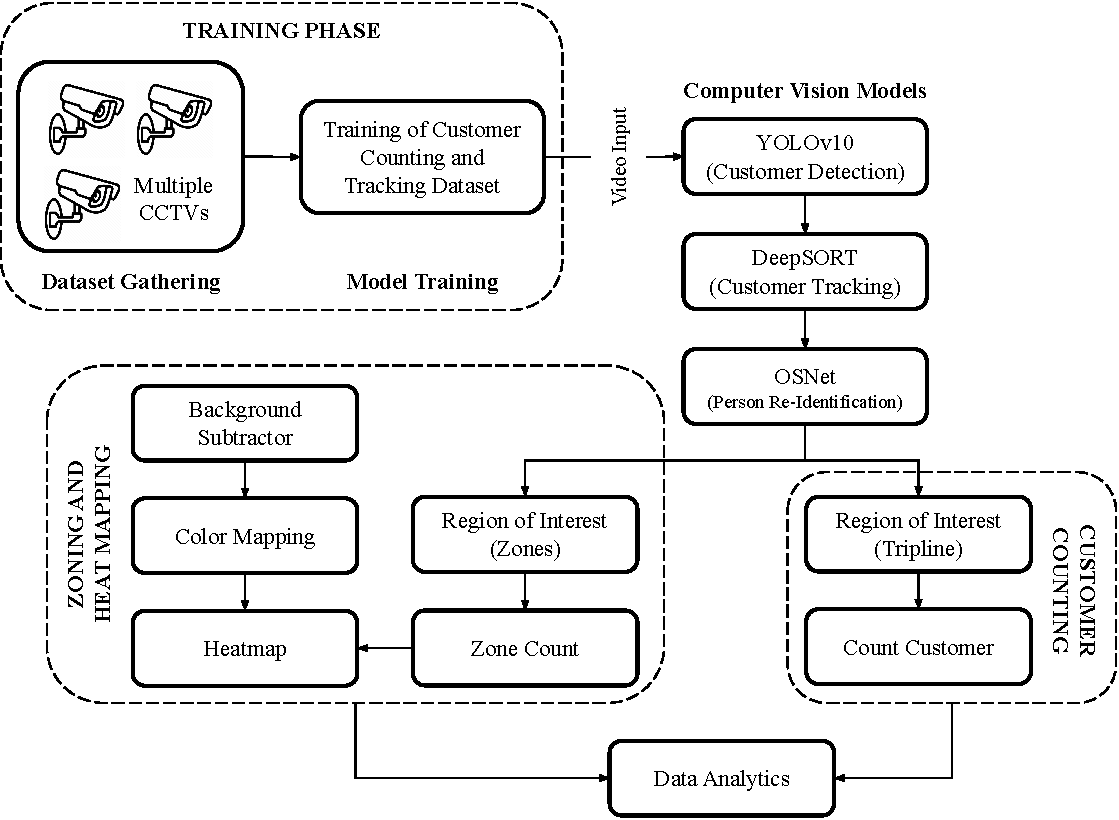
\includegraphics[width=0.85\linewidth]{fig/2.1.pdf}
	\label{fig:2.1}
\end{figure}

}
	
\chapter{METHODOLOGY}
{\baselineskip=2\baselineskip
This chapter discusses the research design and methodology employed in the study. It outlines the procedures for developing, implementing, and evaluating the multi-camera customer tracking system.

\section{Research Design and Procedure}
The study employed an experimental research design, incorporating multiple techniques across various phases to develop and evaluate the proposed system.

\begin{figure}[H]
	\caption[Modified Waterfall Model]{\newline \newline Modified Waterfall Model}
	\centering
	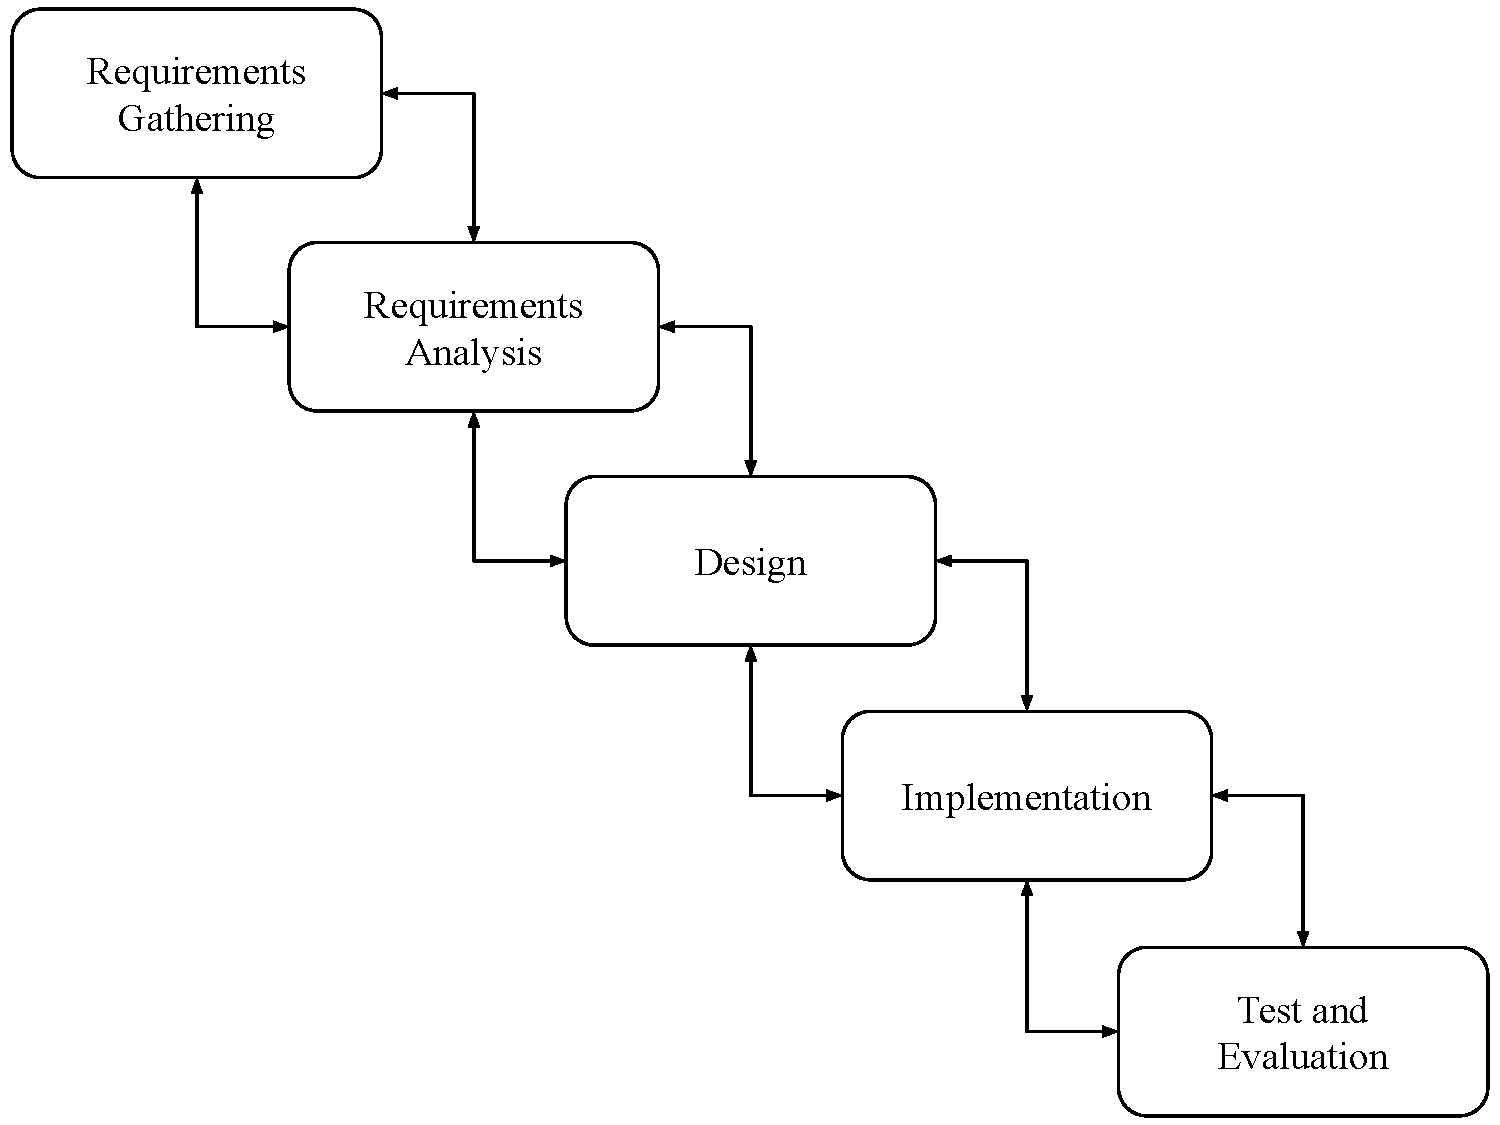
\includegraphics[width=0.7\linewidth]{fig/3.1.pdf}
	\label{fig:3.1}
\end{figure}
This approach enabled systematic testing and refinement through cycles of design, implementation, and assessment. To guide the development process, the researchers adopted a modified Waterfall Model from the System Development Life Cycle (SDLC).

Figure~\ref{fig:3.1} provides a structured framework, promoting a step-by-step progression from requirements gathering to evaluation while allowing for iterative improvements at each stage. The System Design section presents a more detailed discussion of the Modified Waterfall Model, including its phases and adaptations for the study.

\section{Research Setting}

\begin{figure}[H]
	\caption[The Retail Shop in Market City, Agora, Lapasan]{\newline \newline The Retail Shop in Market City, Agora, Lapasan}
	\centering
	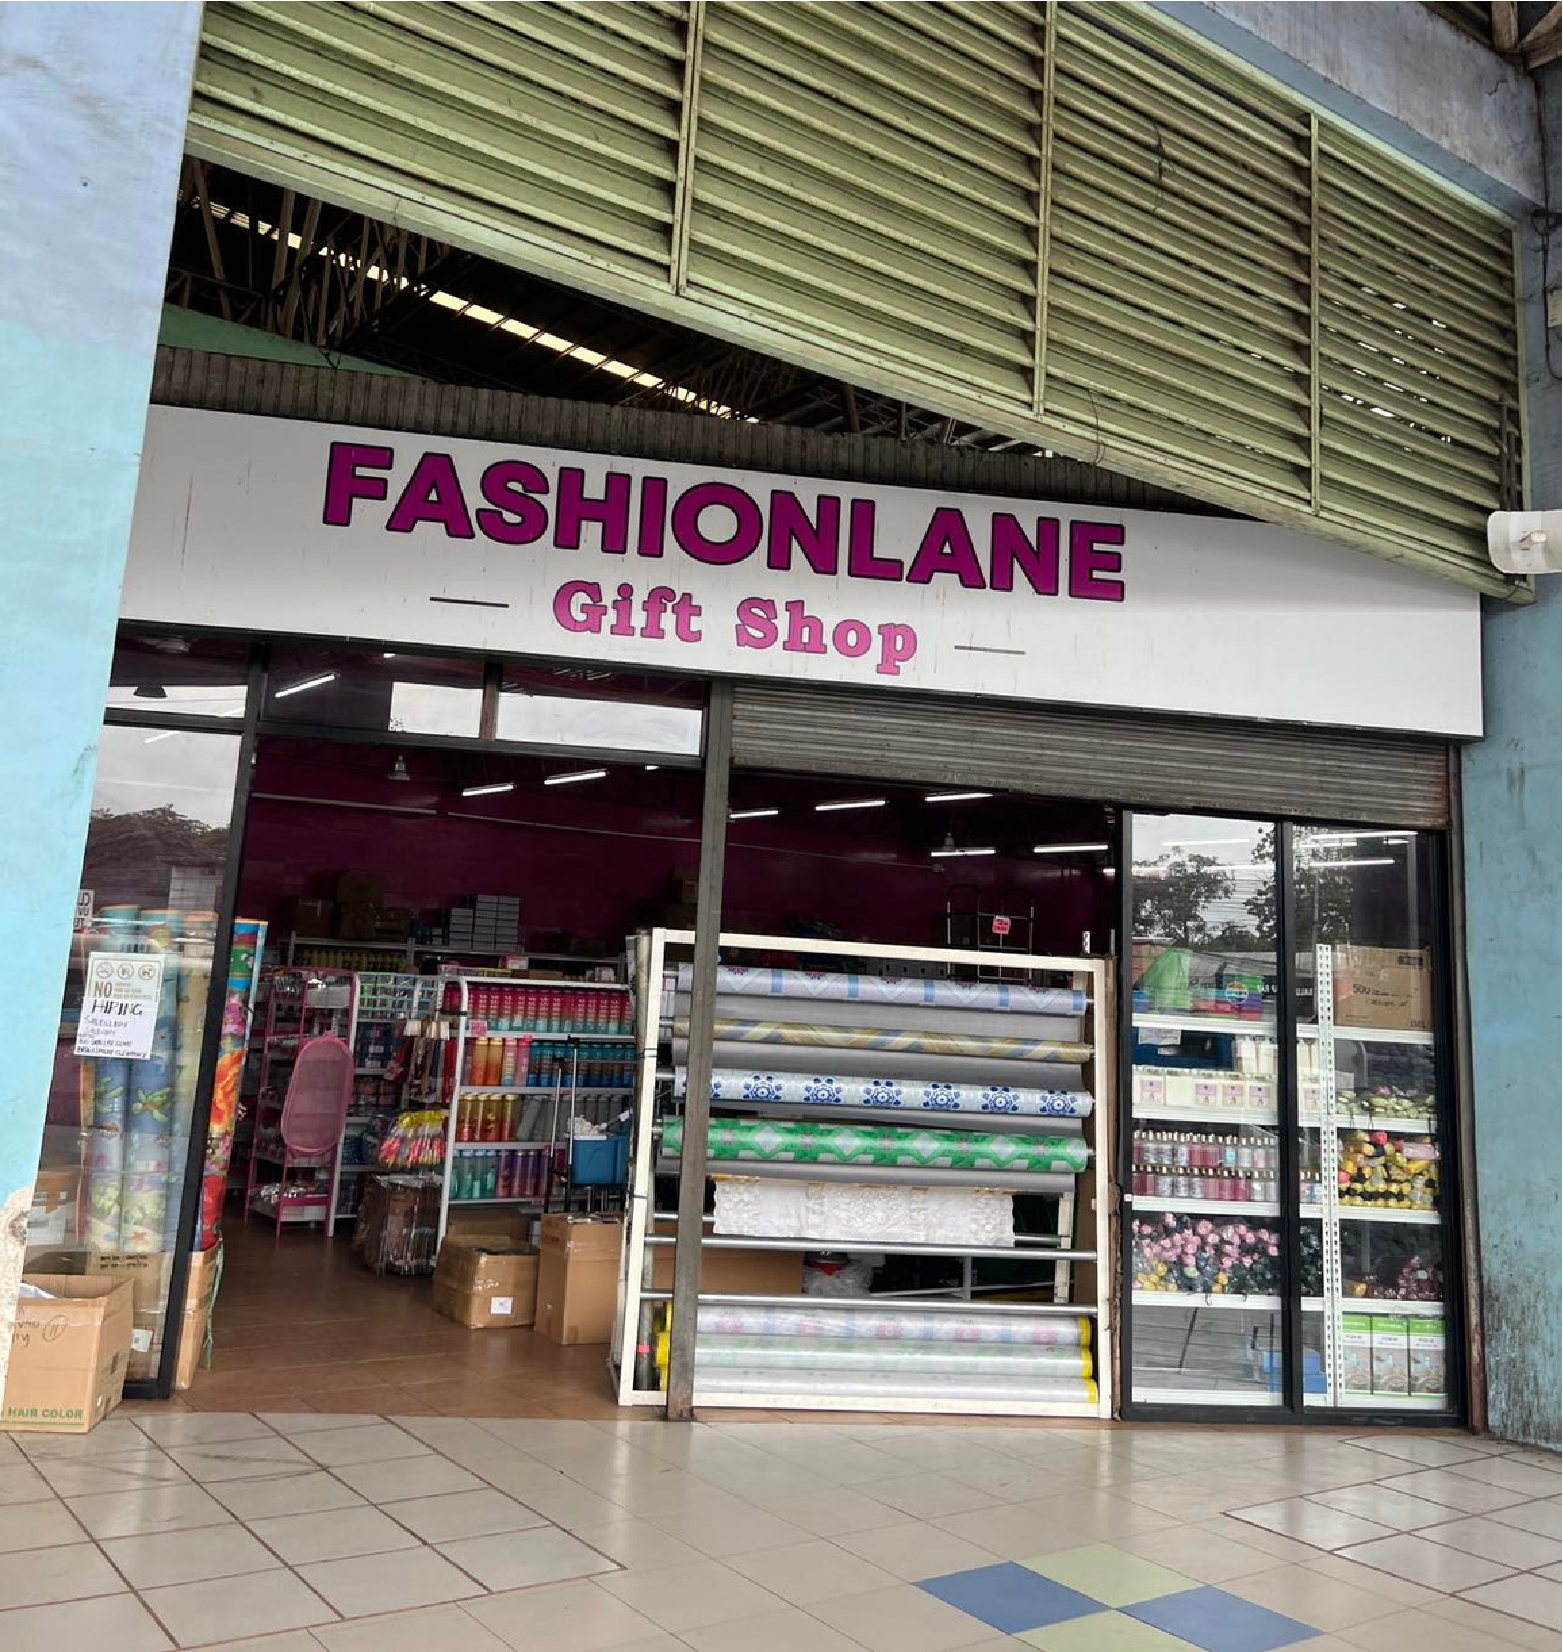
\includegraphics[width=0.5\linewidth]{fig/3.2.pdf}
	\label{figs:3.2}
\end{figure}

The study was conducted at a gift shop located in Market City, Agora, Lapasan, Cagayan de Oro City, shown in Figure~\ref{figs:3.2}. Although the original proposal considered a general merchandise store, the researchers pivoted to the gift shop after assessing its suitability. Despite the change, the store still qualifies as a retail environment, offering a wide range of consumer goods, including body and bath products, cosmetics, school supplies, kitchenware, and home items. Customers freely browse and interact with these products, making it ideal for behavioral observation.

The shop was chosen not only for its product diversity and retail nature but also for its existing CCTV surveillance system, which met the system’s technical requirements. The structured store layout with clear aisles and zones allowed the researchers to define Regions of Interest (ROIs) for tracking movement and behavior. Camera placement covered essential areas like entrances and display zones, requiring only minimal adjustments. Additionally, the store’s location within a busy terminal ensured consistent customer traffic, which was vital for collecting meaningful behavior data. These factors made the gift shop a practical and effective setting for implementing and evaluating the SUBAY system.

\section{Research Setup}

The research setup utilized four existing closed-circuit television (CCTV) cameras from the selected retail environment to ensure comprehensive coverage of key areas. These cameras were strategically positioned to monitor high-traffic zones such as entrances, aisles, and product displays, supporting the requirements of the multi-camera tracking system. Since the surveillance infrastructure was already in place, no additional hardware installation was necessary. Each camera provided a distinct perspective, enabling seamless tracking of customer movement across different sections of the store. Their reliability and high-definition video quality ensured clear footage essential for testing and evaluation.

\begin{figure}[H]
	\caption[Chosen Camera Views Inside the Gift Shop]{\newline \newline Chosen Camera Views Inside the Gift Shop}
	\centering
	\includegraphics[width=1\linewidth]{fig/3.3.pdf}
	\label{fig:3.3}
\end{figure}

Figure~\ref{fig:3.3} presents the selected overlapping camera views (Camera 02, 03, 05, and 09), each strategically chosen for optimal aisle zone visibility, including AISLE 1 through AISLE 6. The layout spans a total distance of 21 meters, with Camera 03 positioned approximately 21 meters from the main aisle area, covering the front desk entrance to minimize obstructions and avoid heavy backlighting. Camera 02 monitors AISLE 1 and AISLE 2, providing visibility of customer movement and interactions near the entrance. Camera 05 covers AISLE 3 and AISLE 4, ensuring high-resolution imaging for accurate detection, while Camera 09 captures AISLE 5 and AISLE 6, completing the surveillance coverage and enhancing overall detection accuracy. The placements were carefully designed to reduce blind spots, maintain image clarity, and optimize performance in varying lighting conditions.

\section{System Design}

This section details the system development process based on the modified Waterfall Model from the System Development Life Cycle (SDLC). It outlines the major phases followed in building the multi-camera customer tracking system, including requirements gathering, analysis, design, implementation, and testing and evaluation.

\subsection{Requirements Gathering}
The requirements gathering process was conducted through an in-person visit and interview with the retail store owner, selected as the primary respondent due to their familiarity with store operations, surveillance practices, and customer behavior. The main objective was to collect essential information for system development and to request formal permission to access the store’s existing CCTV footage.

Before the engagement, the researchers prepared a set of open- and closed-ended questions to guide the discussion, focusing on customer flow, surveillance coverage, and the general store layout. A consent letter outlining the ethical use of the collected data was presented, ensuring that footage and behavioral information would be used solely for academic and research purposes in compliance with data privacy regulations. The store owner reviewed and approved the terms, granting permission to access the CCTV system under agreed conditions.

The interview, conducted on-site with the respondent’s consent, provided insights into camera placements, zones of customer interest, existing challenges in tracking behavior, and the store’s goals for analyzing foot traffic and customer interaction with displays. Complementing the interview, the researchers also conducted field observations, noting customer movement patterns, entry points, checkout counters, and high-interest product areas. The CCTV system was assessed for its coverage, resolution, and timestamp synchronization, all crucial for supporting the proposed tracking and analytics features.

One key insight was the store owner's difficulty in manually interpreting customer activity from raw footage and their interest in an automated solution for analyzing foot traffic and generating behavioral reports. These findings helped define the system’s requirements, ensuring ethical data use while addressing operational needs and aligning with real-world store conditions.

\subsection{Requirements Analysis}
After the requirements gathering process, the researchers compiled and analyzed the data collected from interviews and on-site observations at the retail store. This process enabled them to understand the store’s operational needs, the technological environment, particularly the existing CCTV infrastructure, and the store owner's expectations regarding customer behavior insights.

To support the system’s development and ensure the accuracy of data collection, the researchers were granted secure access to the store's CCTV Video Management Software: iVMS-4200 and Hik-Connect. Access to login credentials and video footage was provided strictly for this study, and all data handling was conducted with strict adherence to privacy protection and confidentiality protocols.

Based on the analysis, the researchers identified the system’s primary users: the Customers and the Retail Store Owner or Manager. While customers are not direct users of the system interface, their behavior and interactions within the store serve as the primary input for the system’s analytical processes. In contrast, the Retail Store Owner or Manager is the principal system user, utilizing the dashboard and generated reports to make informed decisions on store layout and marketing strategies.

\subsubsection{User Definition}

Following the requirements analysis, the system's users were defined as follows:

\textbf{Customers} - Customers are the subjects of data collection. Their movements and interactions within the store are passively monitored through the CCTV infrastructure to generate behavioral analytics.

\textbf{Retail Store Owner/Manager} - The system’s primary user accesses the dashboard, retrieves behavioral reports, and uses the insights generated to optimize store layout and develop marketing strategies.

The specific user requirements are summarized in Table 3.1.

{\setstretch{1.5}
	\begin{longtable}{|p{4cm}|p{11cm}|}
		\caption[User Requirements Table]{\newline \newline User Requirements Table} \label{tab:user-requirements} \\
		\hline
		\textbf{User} & \textbf{Requirement} \\
		\hline
		\endfirsthead
		
		\multicolumn{2}{c}{Table \thetable{} -- continued from previous page} \\
		\hline
		\textbf{User} & \textbf{Requirement} \\
		\hline
		\endhead
		
		\hline \multicolumn{2}{r}{Continued on next page} \\
		\endfoot
		
		\hline
		\endlastfoot
		
		Customer (Indirect) & 
		- Their presence and behavior must be passively and anonymously tracked. \newline
		- Their data must be handled ethically and used solely for research purposes. \\
		\hline
		Retail Store Owner/Manager &
		- Access to a visual dashboard summarizing customer movement and behaviors. \newline
		- Ability to retrieve and download behavioral analytics reports. \newline
		- Tools to analyze foot traffic patterns and product interaction frequency. \newline
		- Insights to support decision-making for store layout and marketing strategies. \newline
		- Ensure that the system does not compromise customer privacy. \\
		\hline
	\end{longtable}
}

This analysis laid the foundation for defining the system’s core features and ensuring that development aligned with both operational needs and ethical considerations.

\subsubsection{System Requirements}
The system requirements, shown in Table~\ref{tab:system-requirements}, were categorized into Input, Process, Output, Control, and Performance specifications to guide system design and implementation.

{\setstretch{1.25}
\begin{longtable}{|p{4cm}|p{11cm}|}
		\caption[System Requirements]{\newline \newline System Requirements Table} \label{tab:system-requirements} \\
		\hline
		\textbf{Category} & \textbf{System Requirement} \\
		\hline
		\endfirsthead
		
		\multicolumn{2}{l}{\tablename\ \thetable{} -- \textit{continued from previous page}} \\
		\hline
		\textbf{Category} & \textbf{System Requirement} \\
		\hline
		\endhead
		
		\hline \multicolumn{2}{|r|}{{Continued on next page}} \\ \hline
		\endfoot
		
		\hline
		\endlastfoot
		
		Input Requirements & 
		- The system shall accept video feeds from the store's existing CCTV infrastructure. \newline
		- The system shall detect and track customer presence in and upon entering the store. \newline
		- The system shall capture customer movement across different store zones. \newline
		- The system shall detect customer visits and dwell time in zones. \newline
		- The system shall log entry/exit points and dwell times automatically. \\*
		\hline
		Process Requirements & 
		- The system shall use object detection (YOLO) and tracking algorithms (DeepSORT) to assign customers unique tracking IDs. \newline
		- The system shall process and analyze customer movement patterns throughout the store. \newline
		- The system shall compile and aggregate behavioral data for further analysis. \newline
		- The system shall anonymize customer data to ensure privacy during processing. \newline
		- The system shall store processed behavioral data in a secure database for future retrieval. \newline
		- The system shall link zone-specific behaviors to product interaction and foot traffic trends. \\
		\hline
		
		Output Requirements & 
		- The system shall display summarized analytics through a visual dashboard. \newline
		- The system shall generate and display foot traffic heat maps and trend charts. \newline
		- The system shall produce downloadable behavioral reports filtered by date range. \newline
		- The system shall show customer interaction metrics such as dwell time per product zone. \\
		\hline
		
		Control Requirements & 
		- The system must secure access through administrator login credentials and restrict sensitive data access to authorized personnel only. \newline
		- The system shall not collect personally identifiable information (PII) from customers (such as social security numbers, full names, email addresses, or phone numbers). \\
		\hline
		
		Performance Requirements & 
		- The system must ensure high accuracy in detecting and tracking customers even in crowded environments. \newline
		- The system shall be capable of handling multiple video feeds simultaneously. \newline
		- The system shall ensure the responsive performance of the dashboard interface and analytics tools. \\
		\hline
		
\end{longtable}
}

The system requirements were developed based on the data collected during the requirements gathering phase. The primary objective of the system is to leverage the store’s existing CCTV infrastructure to anonymously track customer movement and interactions and generate actionable behavioral analytics for the retail store owner. Input requirements focus on collecting movement and interaction data, which are processed using AI-based object detection and tracking algorithms while ensuring customer anonymity. Outputs are presented through an interactive dashboard that provides insights such as foot traffic heat maps, aisle visitation metrics, and customer behavior trends. Control measures guarantee that privacy and data protection standards are strictly observed, while performance requirements ensure the system operates efficiently, accurately, and reliably to support business decision-making.

\subsection{Design}
This section presents the system's design. The researchers worked on a design that would meet the specifications described in the system requirements. To illustrate the system's design, context-level diagrams, data flow diagrams, use case diagrams, activity diagrams, and system architecture were used.

\subsubsection{Context-Level Diagram}
The Context-Level Diagram provides a high-level view of how the SUBAY system interacts with its primary stakeholders: Customers and Retail Store Owners/Managers. It illustrates how data flows into and out of the system without detailing internal processes.

Figure~\ref{fig:3.4} presents the interaction between Customers and the SUBAY system from the perspective of behavioral input and experiential output. While customers do not directly interact with the system, their natural behaviors, such as walking through aisles, pausing at displays, and engaging with products, serve as critical input for SUBAY’s analytics. 

\begin{figure}[H]
	\caption[Context-Level Diagram for Customers]{\newline \newline Context-Level Diagram for Customers}
	\centering
	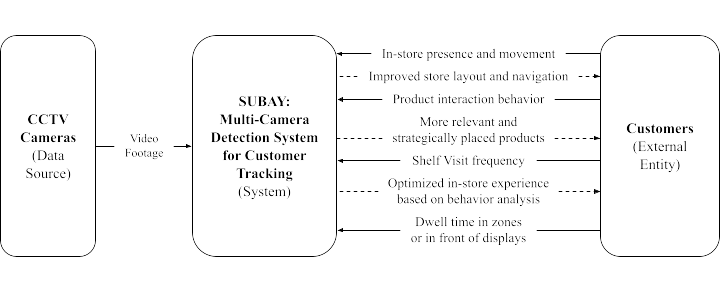
\includegraphics[width=1\linewidth]{fig/3.4.pdf}
	\label{fig:3.4}
\end{figure}

These activities are continuously captured by the existing CCTV infrastructure and analyzed using object detection and multi-camera tracking technologies. The system interprets these behavioral inputs to generate key metrics, including dwell times, zone engagements, visit frequencies, and interaction hotspots. 

\begin{figure}[H]
	\caption[Context-Level Diagram for Retail Store Owners/Managers]{\newline \newline Context-Level Diagram for Retail Store Owners/Managers}
	\centering
	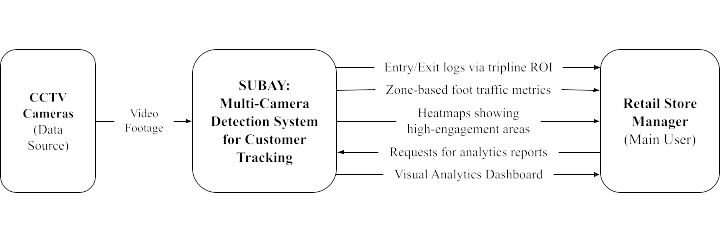
\includegraphics[width=1\linewidth]{fig/3.5.pdf}
	\label{fig:3.5}
\end{figure}

Figure~\ref{fig:3.5} illustrates the system’s interaction with Retail Store Owners and Managers. CCTV cameras are the primary data source, capturing continuous video streams throughout the store. The SUBAY system processes these video feeds to extract actionable insights. The system outputs include entry and exit logs based on tripline detection, zone-based foot traffic analytics, and heat maps highlighting customer engagement patterns. Through a visual analytics dashboard, store owners and managers access metrics, generate customized reports, and make informed decisions about store layouts and marketing initiatives. This context-level view highlights the end-to-end data flow, from passive customer behavior captured on video to strategic insights that empower retail decision-making.

\subsubsection{Data Flow Diagram}

The Data Flow Diagram (DFD) provides a detailed view of how information moves through the SUBAY system, highlighting the key processes that transform raw data into actionable insights for end-users.

\begin{figure}[H]
	\caption[Data Flow Diagram for Customers]{\newline \newline Data Flow Diagram for Customers}
	\centering
	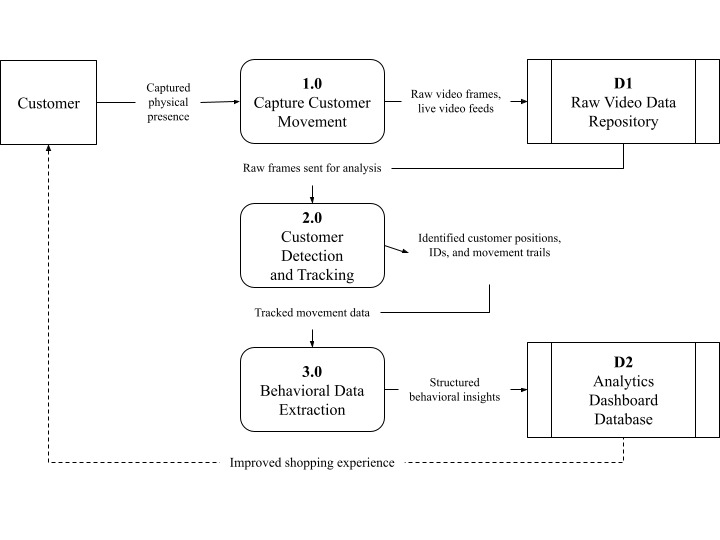
\includegraphics[width=0.80\linewidth]{fig/3.6.pdf}
	\label{fig:3.6}
\end{figure}

\vspace{1em}

Figure~\ref{fig:3.6} illustrates how customer movement within the retail environment initiates the system’s data flow. Without direct input from customers, their presence and actions are captured through continuous video streams. In Process 1.0, these streams are received and prepared for analysis. Process 2.0 applies object detection and multi-camera tracking algorithms to extract movement patterns, paths, and interaction points. The processed movement data is then structured and organized in Process 3.0 before being stored securely in Data Store D2. Although customers remain unaware of these technical operations, the resulting insights significantly improve their shopping experience.

\begin{figure}[H]
	\caption[Data Flow Diagram for Retail Store Owners/Managers]{\newline \newline Data Flow Diagram for Retail Store Owners/Managers}
	\centering
	
\includegraphics[width=1\linewidth]{fig/3.7.pdf}
	\label{fig:3.7}
\end{figure}

Figure~\ref{fig:3.7} presents the Level 1 Data Flow Diagram focused on Retail Store Owners and Managers. The system processes the structured behavioral datasets collected from detection and tracking outputs in Process 1.0 to generate analytical summaries. These summaries are stored in Data Store D1 for retrieval. In Process 2.0, the stored analytics are accessed, organized, and prepared for visualization. Finally, Process 3.0 transforms the data into user-friendly charts, reports, and trend analyses, such as aisles with peak traffic, aisle-specific dwell times, foot traffic charts. Retail store owners access these insights via the dashboard, enabling them to make data-driven decisions.

\subsubsection{Use Case Diagram}
The Use Case Diagram visually represents how different actors interact with the SUBAY system. It captures passive and active engagements that drive data collection and system usage.

\begin{figure}[H]
	\caption[Use Case Diagram for Customers]{\newline \newline Use Case Diagram for Customers}
	\centering
	
\includegraphics[width=0.50\linewidth]{fig/3.8.pdf}
	\label{fig:3.8}
\end{figure}

Figure~\ref{fig:3.8} depicts how shoppers interact indirectly with the retail environment enhanced by SUBAY’s multi-camera detection system. The process begins when a customer enters the store, triggering the initialization of tracking through strategically positioned cameras. As the customer moves across various store zones, the system’s object detection and tracking algorithms monitor and record their paths, dwell times, and interactions with product displays. These interactions are captured passively without disrupting the natural shopping experience. Data such as zone engagement and product interaction durations are aggregated. The insights generated from these behaviors inform store adjustments like layout optimization and targeted promotions.

\begin{figure}[H]
	\caption[Use Case Diagram for Retail Store Owners/Managers]{\newline \newline Use Case Diagram for Retail Store Owners/Managers}
	\centering
	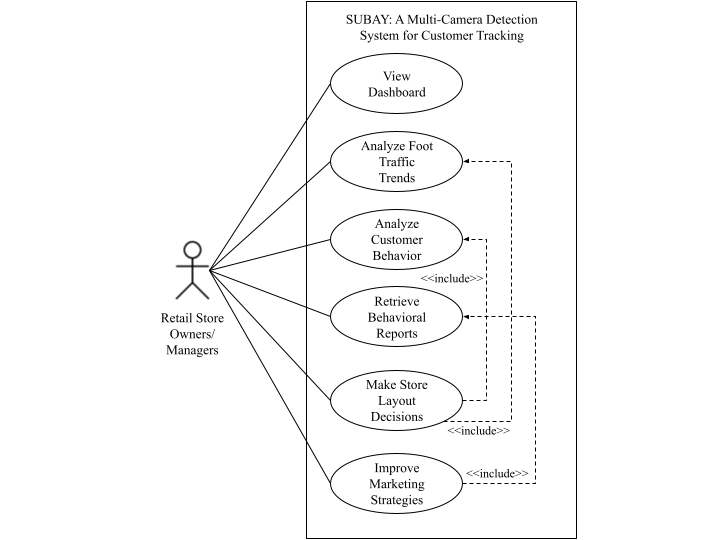
\includegraphics[width=1\linewidth]{fig/3.9.pdf}
	\label{fig:3.9}
\end{figure}

Figure~\ref{fig:3.9} illustrates the interaction between retail store owners or managers and the SUBAY system. Users can view the dashboard to access customer tracking insights. From this central interface, they can analyze zone-specific foot traffic and dwell time trends, which are included use cases essential for data-driven decision-making. These analytics support key business activities such as making store layout decisions and improving marketing strategies. Additionally, the system enables retrieval of detailed insight reports, helping managers better understand customer behavior. The use case relationships demonstrate how SUBAY streamlines customer analytics to help store owners optimize operations and enhance the overall shopping experience.

\subsubsection{Activity Diagram}

The Activity Diagram details the sequence of operations within the SUBAY system, highlighting the dynamic flow of actions between the system and its users.

\begin{figure}[H]
	\caption[Activity Diagram for Customers]{\newline \newline Activity Diagram for Customers}
	\centering
	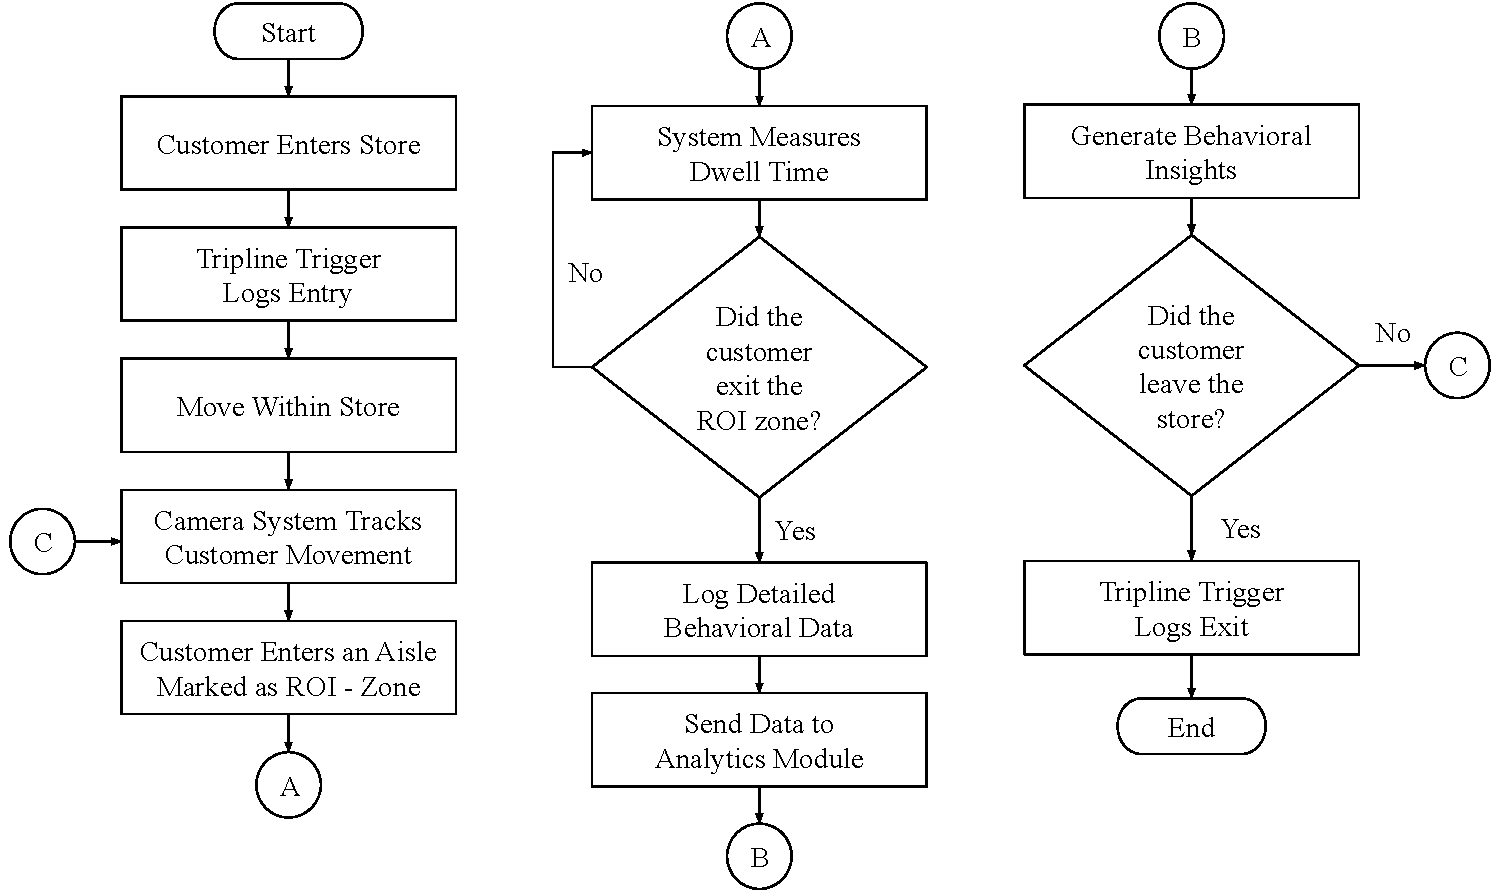
\includegraphics[width=0.75\linewidth]{fig/3.10.pdf}
	\label{fig:3.10}
\end{figure}

Figure~\ref{fig:3.10} illustrates the customer activity flow within the retail environment. The process begins when a customer enters the store, automatically triggering the customer-counting system, which logs their entry. As the customer navigates the store, the system passively monitors their movement. When customers enter a designated zone and interact with product displays, the system measures their dwell time. If the customer remains in the zone, dwell time is continuously recorded; otherwise, if they move out, the system logs the interaction and resumes tracking across other zones. Upon exiting the store, the system records their departure, closing the tracking session.

\begin{figure}[H]
	\caption[ Activity Diagram for Retail Store Owners/Managers]{\newline \newline Activity Diagram for Retail Store Owners/Managers}
	\centering
	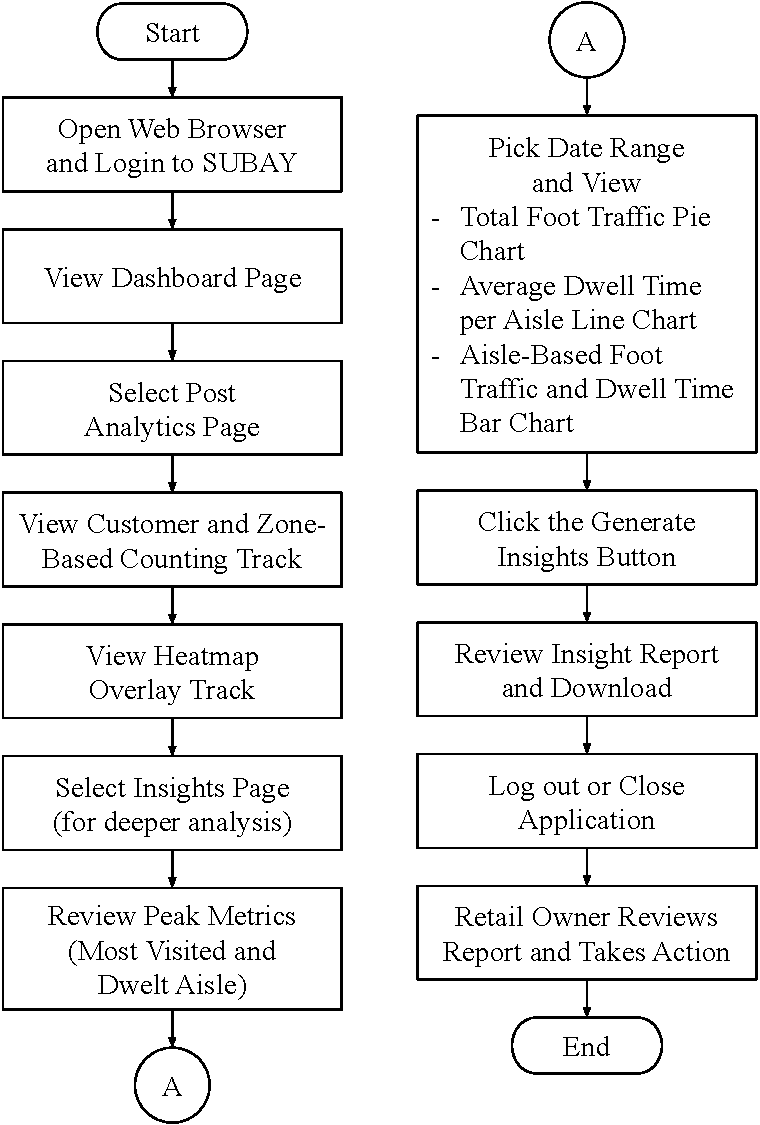
\includegraphics[width=0.40\linewidth]{fig/3.11.pdf}
	\label{fig:3.11}
\end{figure}

The activity diagram as shown on Figure~\ref{fig:3.11} illustrates the typical user flow for retail store owners or managers utilizing the SUBAY system. It begins with accessing the web application and navigating through the dashboard to the Post Analytics and Insights pages. Users can explore zone-based customer counts, heatmaps, and peak metrics such as the most visited and dwell aisles. The process continues with selecting a date range and generating charts that visualize total foot traffic, average dwell time, and zone-specific interactions. A detailed diagram for the insight generation phase will be presented to elaborate on this process. Finally, reports are reviewed and acted upon accordingly.

\begin{figure}[H]
	\caption[Insight Generation Activity Diagram]{\newline \newline Insight Generation Activity Diagram}
	\centering
	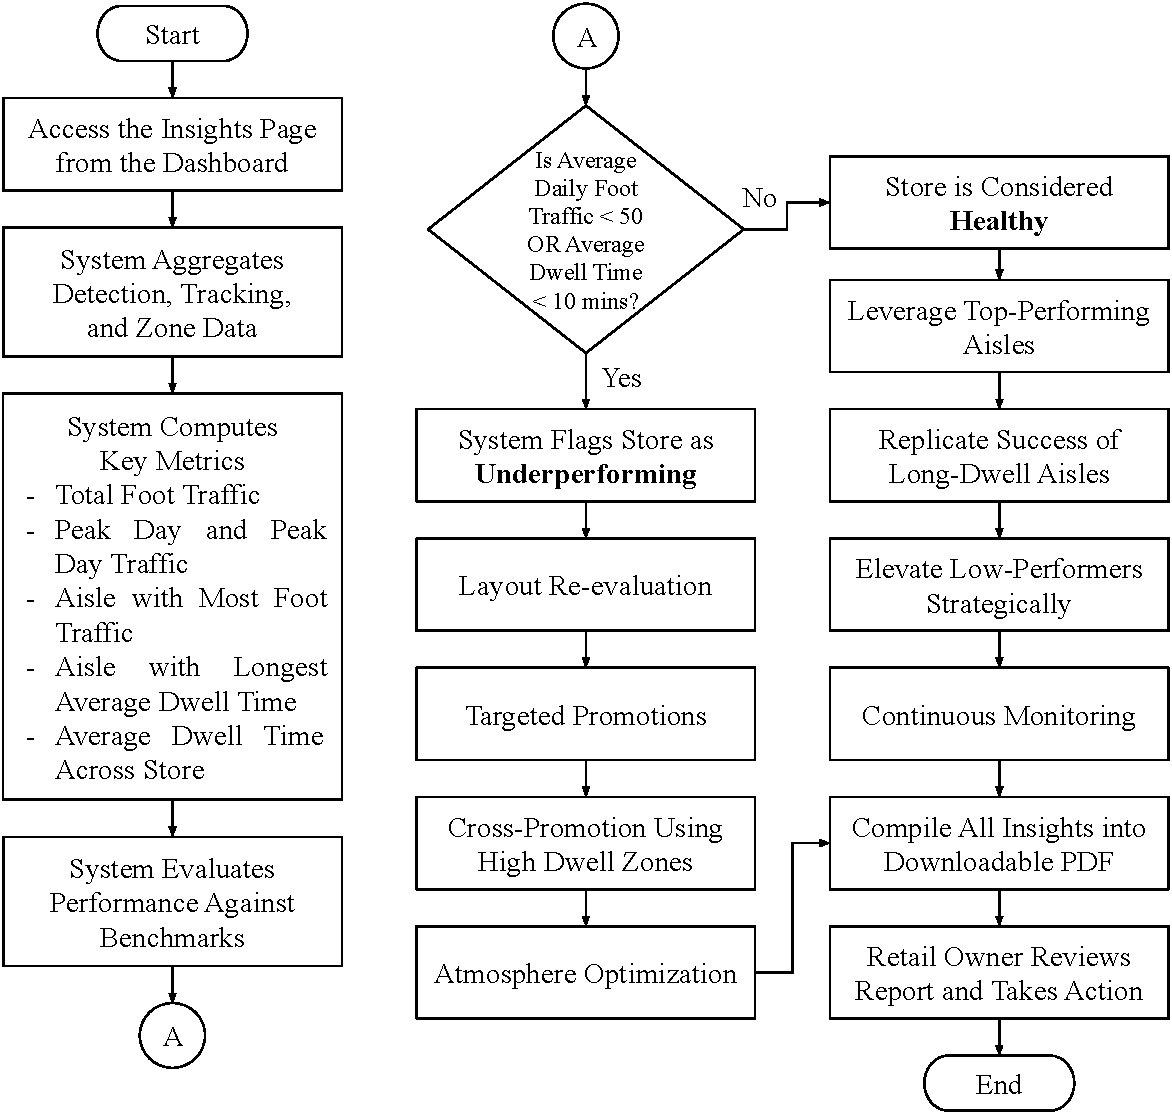
\includegraphics[width=0.80\linewidth]{fig/3.12.pdf}
	\label{fig:3.12}
\end{figure}

As shown in Figure~\ref{fig:3.12}, upon navigating the Insights Page, the system automatically processes all collected behavioral data from previous detection, tracking, and zone monitoring. Using the backend datasets, it computes essential performance metrics, including the total number of customer entries (foot traffic) during the monitored period, the peak day in terms of entries, zone-specific traffic volumes, average and peak dwell times, and the percentage breakdown of visits per zone. These metrics are evaluated against industry-aligned benchmarks: a daily average foot traffic threshold of 50 customers and an average dwell time of 10 minutes. These values were based on research from sources like \cite{BPlanAI2025} and \cite{CountTrack2025}, which identify underperformance in gift shops, especially those selling beauty and home products, when engagement or movement is below these thresholds.

\noindent\textbf{If the Store Is Flagged as Underperforming}

If averageDailyFootTraffic $<$ 50 or averageCustomerDwellTime $<$ 10 mins, the system concludes that the store is currently underperforming and automatically generates the following insights and actions based on the suggestions and recommendations in the articles by \cite{BPlanAI2025} and \cite{CountTrack2025}:

\textbf{Layout Re-evaluation:} The system suggests reassessing the spatial layout of underperforming aisles (e.g., Aisle C or D). The store manager may consider widening tight spaces, rearranging congested product racks, and improving line-of-sight to make items more visible and accessible. For instance, if Aisle C only had 5\% of the traffic, products might be moved closer to high-traffic intersections to boost exposure.

\textbf{Targeted Promotions:} Promotions such as discounts or bundle deals can be introduced in these low-traffic zones to encourage customer exploration. The system recommends prioritizing aisles with low visits and dwell time, suggesting that neither foot traffic nor customer interest is sustained in those sections.

\textbf{Cross-Promotion Using High Dwell Zones:} If Aisle A had the longest dwell time, the system recommends placing high-margin or complementary items (e.g., perfumes near hair care products) in that zone or its vicinity. Customers tend to linger where they’re intrigued, leveraging this zone to promote slower-moving products improves overall conversion.

\textbf{Atmosphere Optimization:} The system recommends better lighting, cleaner aisle signage, or even thematic decorations to attract attention. Aesthetic enhancements can invite customers into previously ignored areas.

\noindent\textbf{If the Store Is Performing Well}

If averageDailyFootTraffic $\geq$ 50 and averageCustomerDwellTime $\geq$ 10 minutes, the system concludes healthy engagement and provides insights to maintain or amplify success based on the suggestions and recommendations in the articles by \cite{BPlanAI2025} and \cite{CountTrack2025}:

\textbf{Leverage Top-Performing Aisles:} If Aisle B had 30\% of total foot traffic, placing promotional stands or new arrivals here could maximize reach and conversions. Popular aisles should act as marketing touchpoints.

\textbf{Replicate Success of Long-Dwell Aisles:} If Aisle A has a 40-minute average dwell time, the system recommends analyzing its product types, lighting, arrangement, and spacing. These characteristics can be mirrored in other aisles to boost performance.

\textbf{Elevate Low-Performers Strategically:} The system doesn’t ignore low-performing areas even if the store is healthy overall. Recommendations include mirroring top aisle attributes or rotating products to test customer response.

\textbf{Continuous Monitoring:} Managers are encouraged to monitor these metrics weekly, noting changes during promotional events, holidays, or layout changes. This supports evidence-based adjustments over time.

\subsubsection{System Architecture}
This section presents the system architecture. It illustrates the services, layers, components, architecture, and interactions and serves as the physical blueprint of the system.

Figure~\ref{fig:3.13} below illustrates the complete system architecture of SUBAY. The process begins with video footage captured from four strategically placed CCTV cameras. These video streams are processed through a detection module utilizing the YOLOv10 model, known for its high accuracy in detecting individuals. Following detection, the DeepSORT tracking algorithm maintains consistent tracking of individuals across multiple frames and camera views, enabling reliable mapping of customer movement throughout the store. The store layout is divided into predefined zones, allowing the system to focus behavioral analysis on specific areas. Movement patterns, zone occupancy, and customer flow are systematically captured and analyzed.

A heat mapping module further enriches this analysis by visualizing dwell time and movement intensity, using color gradients to highlight areas of high customer engagement. All collected behavioral data, including foot traffic metrics, zone visits, dwell time, and heat map visuals, are transmitted to an analytics dashboard. 

\begin{figure}[H]
\	\caption[System Architecture]{\newline \newline System Architecture}
	\centering
	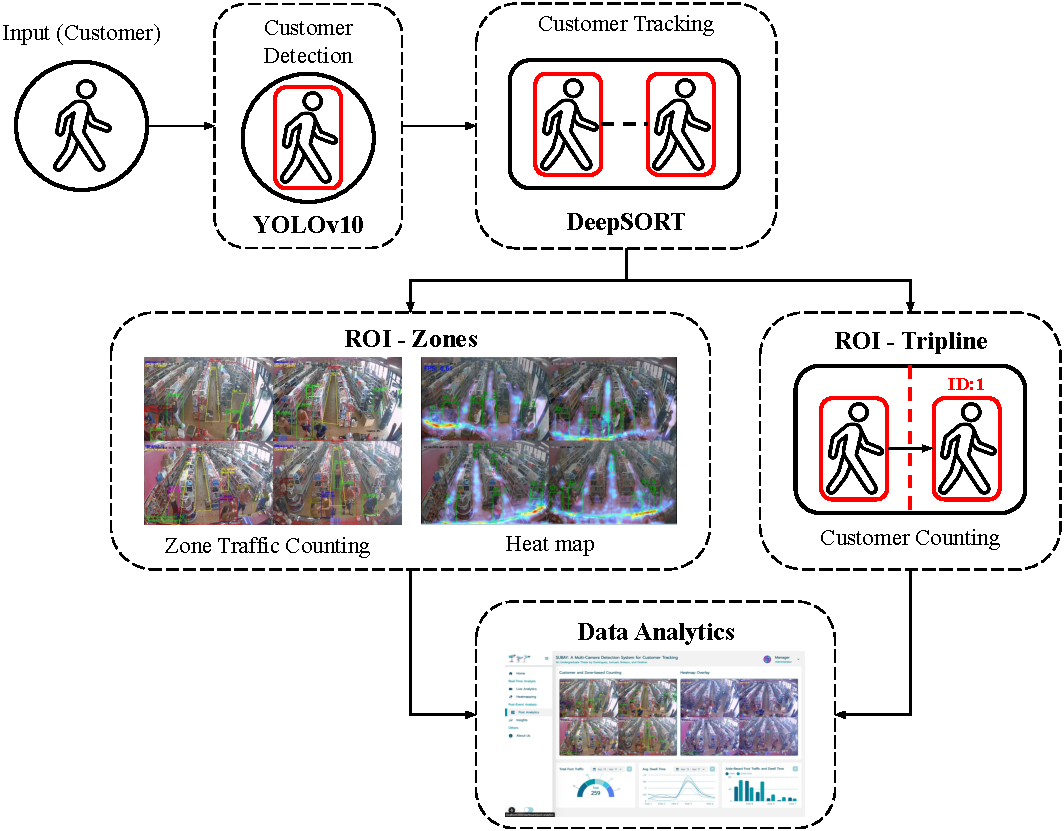
\includegraphics[width=1\linewidth]{fig/3.13.pdf}
	\label{fig:3.13}
\end{figure}

This dashboard serves as the primary interface for retail managers, presenting data in user-friendly visual formats. Managers can monitor foot traffic trends through the dashboard, evaluate zone effectiveness, and gain deeper insights into customer behaviors. These insights support strategic decisions on store layout optimization and product placement, ultimately boosting their sales performance.

\subsection{Implementation}

The implementation phase focused on developing the software components of the SUBAY system, leveraging the store’s existing CCTV infrastructure as the primary video input source. This minimized setup complexity and facilitated seamless integration into the retail environment.

\begin{figure}[H]
	\caption[Steps in Implementing SUBAY]{\newline \newline Steps in Implementing SUBAY}
	\centering
	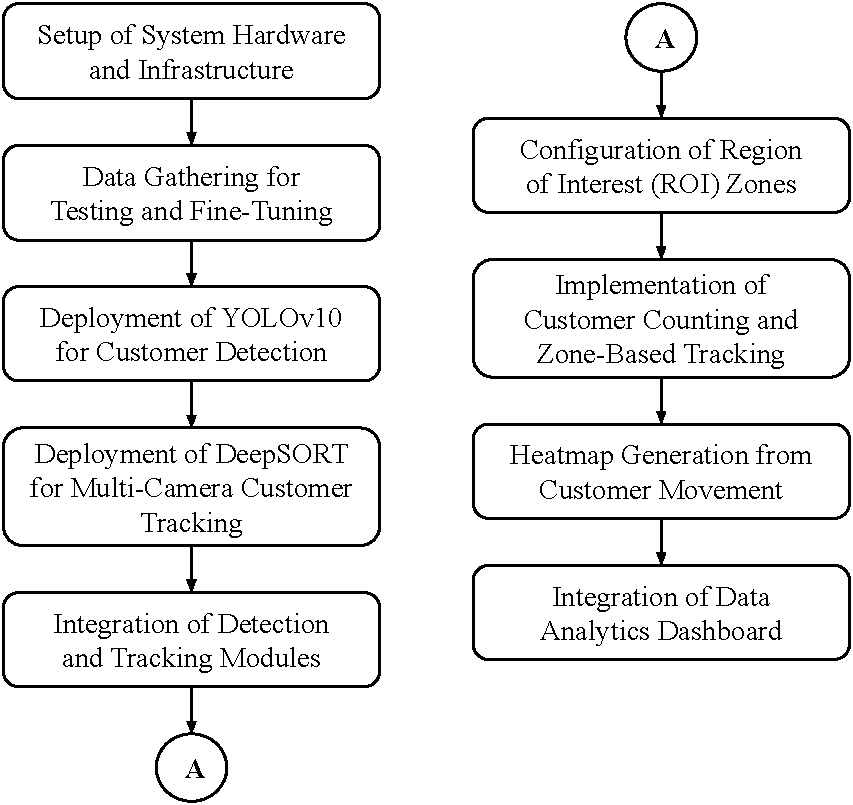
\includegraphics[width=0.50\linewidth]{fig/3.14.pdf}
	\label{fig:3.14}
\end{figure}

As illustrated in Figure~\ref{fig:3.14}, the implementation began by configuring a high-performance computing (HPC) unit designed to handle the computational demands of real-time video processing. The system followed a structured pipeline: customer detection, tracking, re-identification, zone monitoring, and behavioral data aggregation. The first stage involved deploying YOLOv10, a deep learning object detection model, to accurately localize individuals within each video frame captured from multiple cameras. Detected customers were then passed to DeepSORT, an advanced tracking algorithm, to assign and maintain unique identities as they moved across camera views. DeepSORT was enhanced with OSNet, a person re-identification model that preserved identity consistency even under occlusion, lighting changes, and camera transitions for added robustness.

Regions of Interest (ROIs) were manually defined across strategic areas such as aisles and product shelves to enable zone-based analytics. The system continuously monitored customer presence within these zones, calculated dwell time, and generated active customer counts based on the assigned tracking IDs. These behavioral metrics were visualized through heat maps using color gradients to represent spatial engagement and movement density. All outputs, including customer counts, zone engagement, dwell time, and heat maps, were integrated into the SUBAY analytics dashboard. This dashboard served as the final interface for retail managers, offering an intuitive view of customer behavior to support layout optimization and data-driven promotional strategies.

The development environment employed two primary configurations: Microsoft Visual Studio Code IDE for structured Python code development and debugging, and a Linux-based HPC text editor for resource-efficiently executing training scripts and video processing pipelines. The system was built on a robust and modular software stack. Python served as the primary development language, with PyTorch used for deep learning operations, TorchReID for re-identification, and OpenCV and NumPy for computer vision and numerical processing. The motion prediction and data association tasks were handled using the Kalman Filter and the Hungarian Algorithm. Visual outputs such as heat maps were refined for clarity using Gaussian-based rendering, alpha blending, and morphological operations.

To achieve high-speed processing and reliable performance, the system utilized CUDA-enabled GPU acceleration and multithreaded execution through ThreadPoolExecutor and Threading. Tracking accuracy was further improved through Cosine Similarity and Intersection over Union (IoU) metrics. YAML configuration files were used to streamline model and system parameter settings. This implementation strategy enabled SUBAY to process video feeds, track customers accurately across multiple views, and generate actionable behavioral analytics with speed, precision, and efficiency.

\subsubsection{Customer Detection}

The implementation of customer detection in this study centered on deploying a convolutional neural network (CNN)-based object detection model, You Only Look Once version 10 (YOLOv10). YOLOv10 served as the foundation of the system’s detection pipeline, identifying customers from video input captured by four pre-installed CCTV cameras positioned at store entrances, aisles, and display zones. This setup provided continuous coverage without requiring additional hardware installation.

Video feeds were processed frame by frame, where YOLOv10 generated bounding boxes, class labels, and confidence scores to detect and localize individuals. These outputs allowed the system to highlight customers’ positions within each frame while filtering out non-customer objects and background noise.

To improve detection performance under real-world conditions, the model was periodically fine-tuned using additional footage from the store itself. This incremental training allowed the system to adapt to variations in lighting, customer appearance, and crowd density, ensuring consistent detection accuracy.

\begin{figure}[H]
	\caption[The Architecture of YOLO CNN \citep{Artamonov2018}]{\newline \newline The Architecture of YOLO CNN \citep{Artamonov2018}}
	\centering
	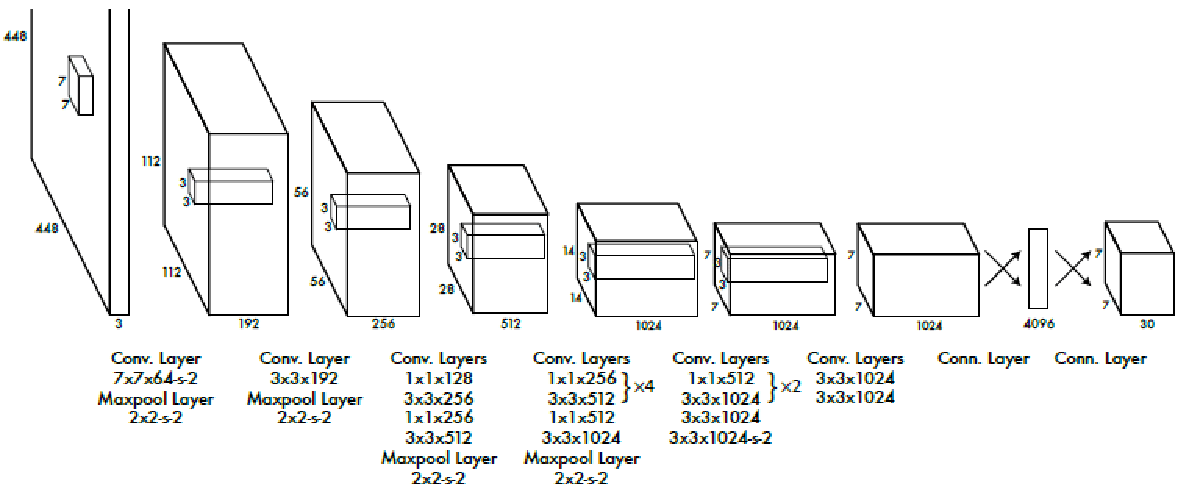
\includegraphics[width=1\linewidth]{fig/3.15.pdf}
	\label{fig:3.15}
\end{figure}

As shown in Figure~\ref{fig:3.15}, the detection process started with YOLOv10 extracting spatial features from each frame through a series of convolutional layers. The detected individuals were then passed to the tracking module, where they were assigned persistent IDs for continuous monitoring across frames and cameras. This seamless flow between detection and tracking enabled reliable zone monitoring, heat mapping, and analytics generation.

Figure~\ref{fig:3.16} outlines the customer classification process used in the system. Video streams were broken into frames and analyzed to detect entities such as shelves, carts, and people, each labeled with a confidence score. An object filtering stage was applied to remove false positives based on size, movement, and location criteria. Detections showing human-like movement and features were classified as customers.

\begin{figure}[H]
	\caption[Classifying Customers Diagram]{\newline \newline Classifying Customers Diagram}
	\centering
	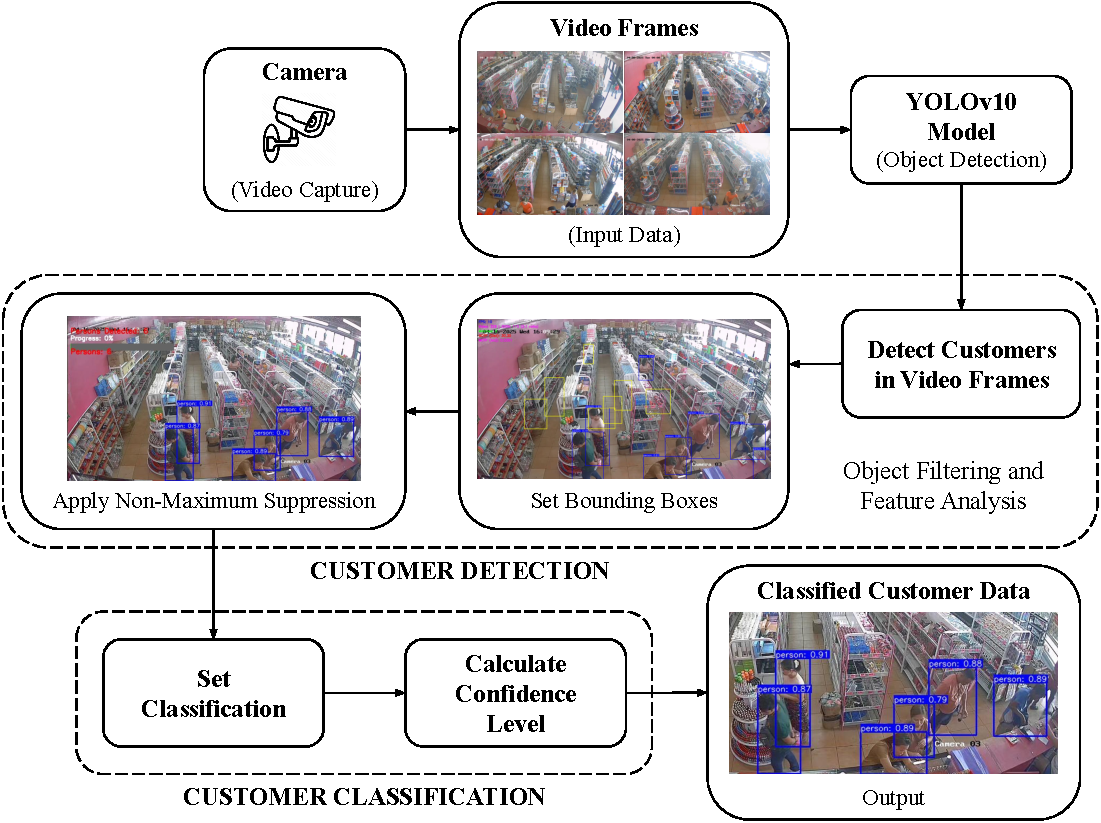
\includegraphics[width=0.75\linewidth]{fig/3.16.pdf}
	\label{fig:3.16}
\end{figure}

A confidence scoring module evaluated detection reliability by considering motion patterns, object shape, and clarity. Verified customers were then assigned a unique ID, spatial coordinates, and a classification confidence score. Only these structured, high-confidence detections were passed to downstream modules for tracking, counting, zone analysis, and heat map generation, ensuring the system’s outputs remained accurate and actionable.

\subsubsection{Customer Tracking}

To maintain persistent identification of customers throughout their in-store journey, the system combined YOLOv10 for object detection with DeepSORT for object tracking. This integration allowed accurate monitoring of individuals across frames, even when partial occlusion, camera switching, or brief disappearances occurred.

While YOLOv10 localized customers in single frames, it could not associate their identities over time. DeepSORT addressed this by introducing a deep Re-Identification (Re-ID) model, which extracted appearance features from each detected individual. These features matched identities across frames, reducing ID-switching and ensuring consistent tracking.

\begin{figure}[H]
	\caption[DeepSORT: SORT with a Deep Association Metric \citep{Admin2023}]{\newline \newline DeepSORT: SORT with a Deep Association Metric \citep{Admin2023}}
	\centering
	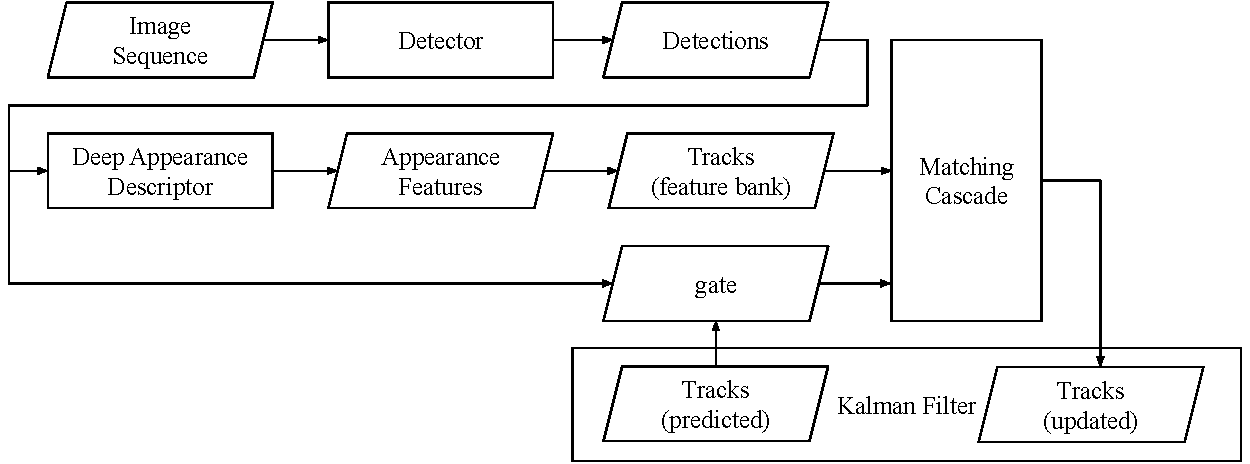
\includegraphics[width=0.75\linewidth]{fig/3.17.pdf}
	\label{fig:3.17}
\end{figure}

As shown in Figure~\ref{fig:3.17}, detection outputs from YOLOv10 were passed through a feature extractor to generate appearance vectors. These vectors were compared with existing tracked identities using a matching cascade based on appearance similarity and motion predictions. A Kalman filter refined the estimated locations, integrating new detection data with past movement patterns to maintain stable and smooth trajectories.

Figure~\ref{fig:3.18} below illustrates the assignment and maintenance of unique customer IDs. Upon detection, individuals were given a persistent ID consistent across frames and camera views. If a visual match was found based on features like color, shape, and motion, the ID and trajectory were updated; otherwise, a new ID was assigned. This process prevented duplication and maintained accurate tracking continuity.

\begin{figure}[H]
	\caption[Tracking Customer IDs]{\newline \newline Tracking Customer IDs}
	\centering
	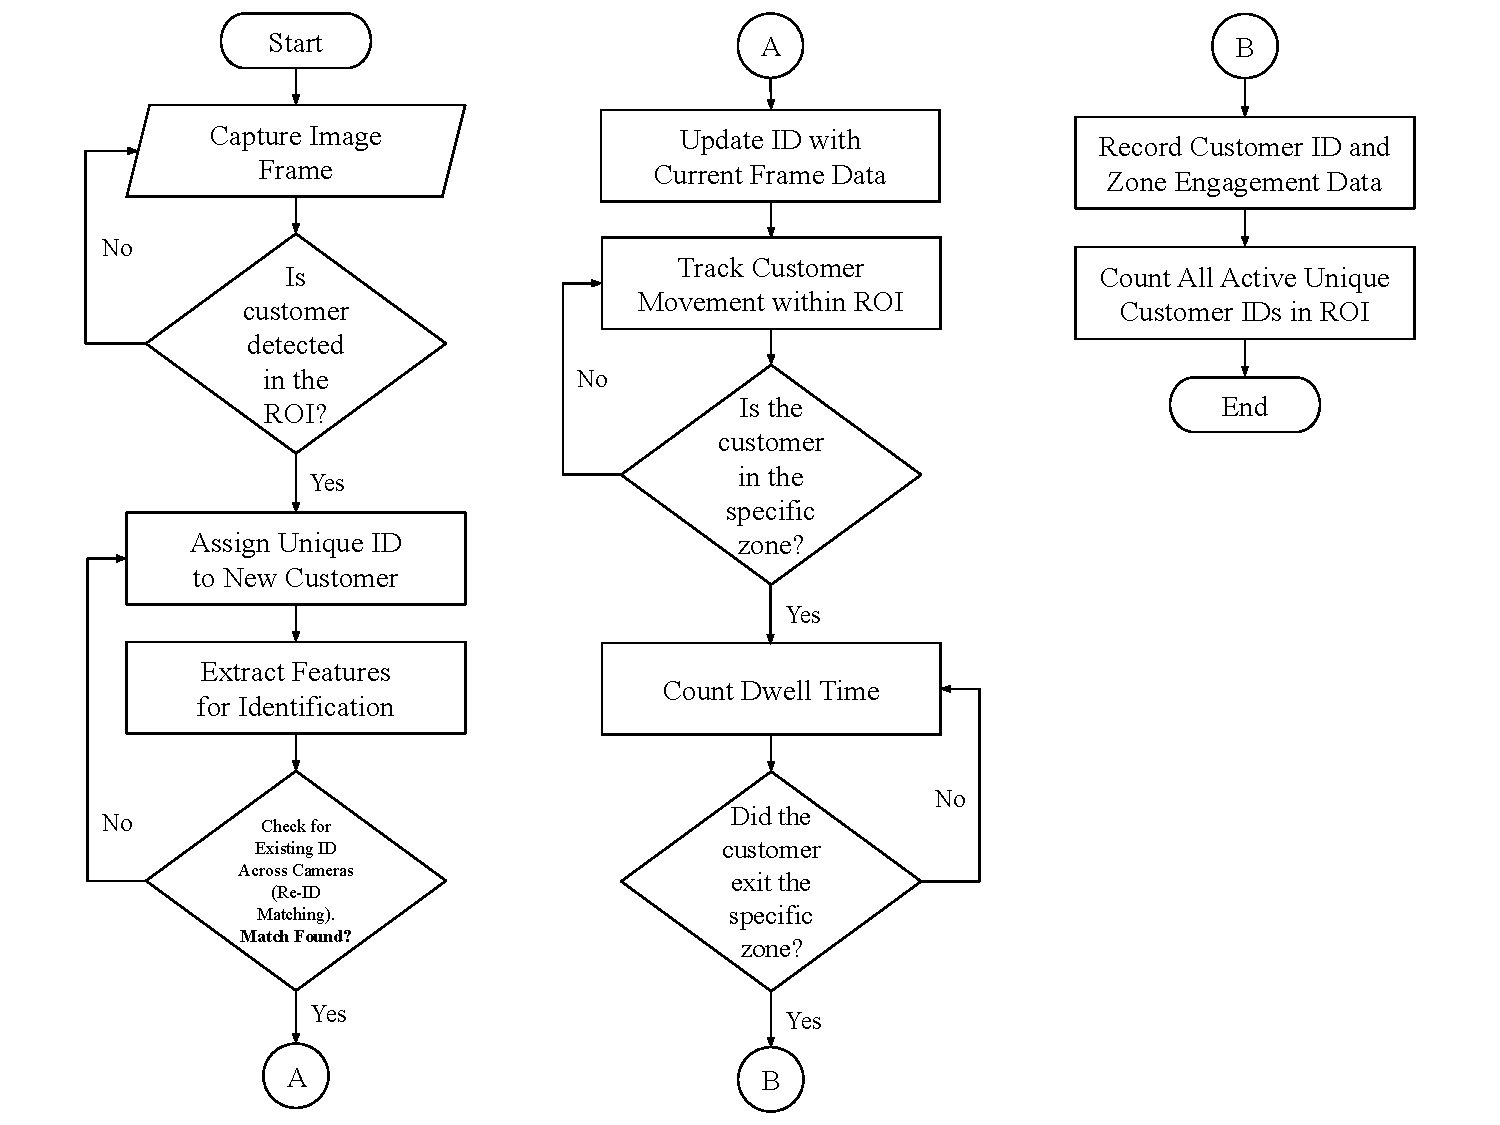
\includegraphics[width=1\linewidth]{figs/3.18.pdf}
	\label{fig:3.18}
\end{figure}

DeepSORT is effective for tracking individuals within a single camera stream; however, it struggles to maintain consistent identity tracking across multiple camera frames, especially when individuals move between non-overlapping fields of view. The system integrated OSNet (Omni-Scale Network) into the DeepSORT pipeline to overcome this limitation and improve person re-identification (Re-ID) across cameras. OSNet enhances identity recognition by capturing fine-grained and global appearance features through multiple convolutional streams within a single residual block. As illustrated in Figure~\ref{fig:3.19}, its unified aggregation gate adaptively prioritizes relevant features, improving robustness to occlusion, pose variation, and lighting differences.

\begin{figure}[H]
	\caption[A Schematic of the Proposed Building Block for OSNet. R: Receptive field size. \citep{Boujou2022}]{\newline \newline A Schematic of the Proposed Building Block for OSNet. R: Receptive field size. \citep{Boujou2022}}
	\centering
	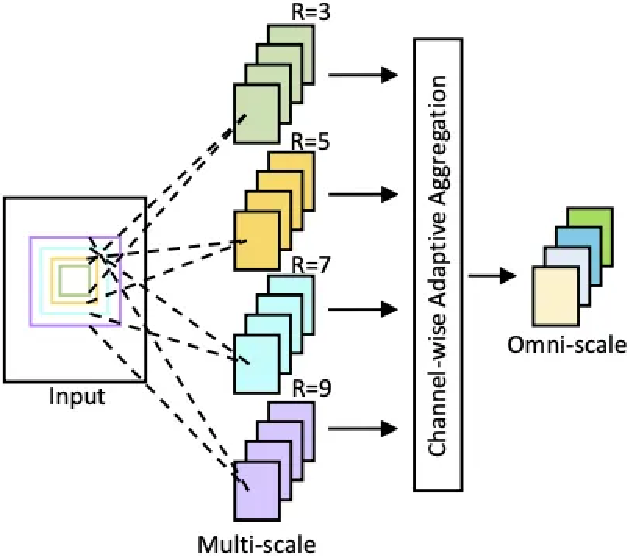
\includegraphics[width=0.50\linewidth]{fig/3.19}
	\label{fig:3.19}
\end{figure}

Despite its detailed feature extraction, OSNet remained computationally efficient, making it ideal for retail applications. By leveraging OSNet, the system achieved consistent identity matching across different camera angles and challenging conditions. As customers moved through predefined Regions of Interest (ROIs), the system tracked entries, dwell times, and movement paths. These tracking records were later used to generate zone engagement metrics and behavioral flow analysis, supporting data-driven retail decision-making.

\subsubsection{Customer Counting}

The SUBAY system combined object detection with multi-object tracking to accurately measure foot traffic, moving beyond traditional tripline-only methods. Instead of relying solely on fixed lines, it used intelligent detection and tracking across multiple camera views to prevent redundant or missed counts.

As shown in Figure~\ref{fig:3.20}, the process began with video streams from the store’s CCTV cameras. YOLOv10 detected individuals frame by frame, while DeepSORT tracked them across multiple frames and angles. A Region of Interest (ROI) tripline was placed at a key entrance view to identify new customer entries.

\begin{figure}[H]
	\caption[Customer Counting Process]{\newline \newline Customer Counting Process}
	\centering
	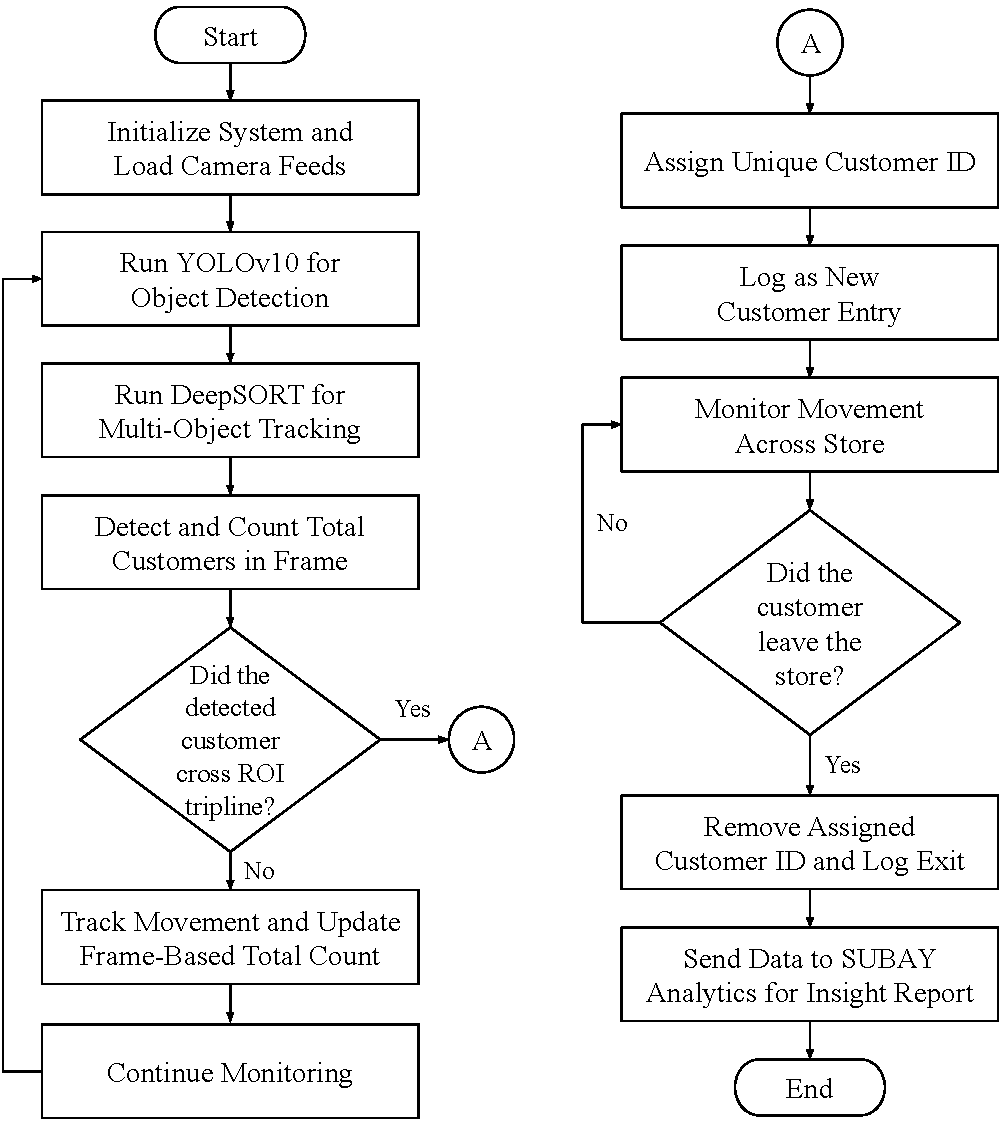
\includegraphics[width=0.50\linewidth]{fig/3.20.pdf}
	\label{fig:3.20}
\end{figure}

When a detected individual crossed the tripline in the correct direction, the system logged the event as a new entry and assigned a unique ID for tracking. This ID remained active while the customer stayed inside and was discarded upon exit. The system maintained reliable, non-redundant entry counts by combining continuous frame-based monitoring with directional tripline detection. All collected counting data, including current presence and cumulative foot traffic, was forwarded to the SUBAY analytics dashboard to support operational insights and store performance evaluation.

The system maintained reliable, non-redundant entry counts by combining continuous frame-based monitoring with directional tripline detection. All collected counting data, including current presence and cumulative foot traffic, was forwarded to the SUBAY analytics dashboard to support operational insights and store performance evaluation.

\subsubsection{Zoning and Heat Mapping}

The SUBAY system implemented zone monitoring based on predefined Regions of Interest (ROIs) to better understand how customers interacted with specific areas. These zones were mapped onto camera views covering important retail spaces like aisles and product displays.

\begin{figure}[H]
	\caption[Customer Counting Inside Zone Process]{\newline \newline Customer Counting Inside Zone Process}
	\centering
	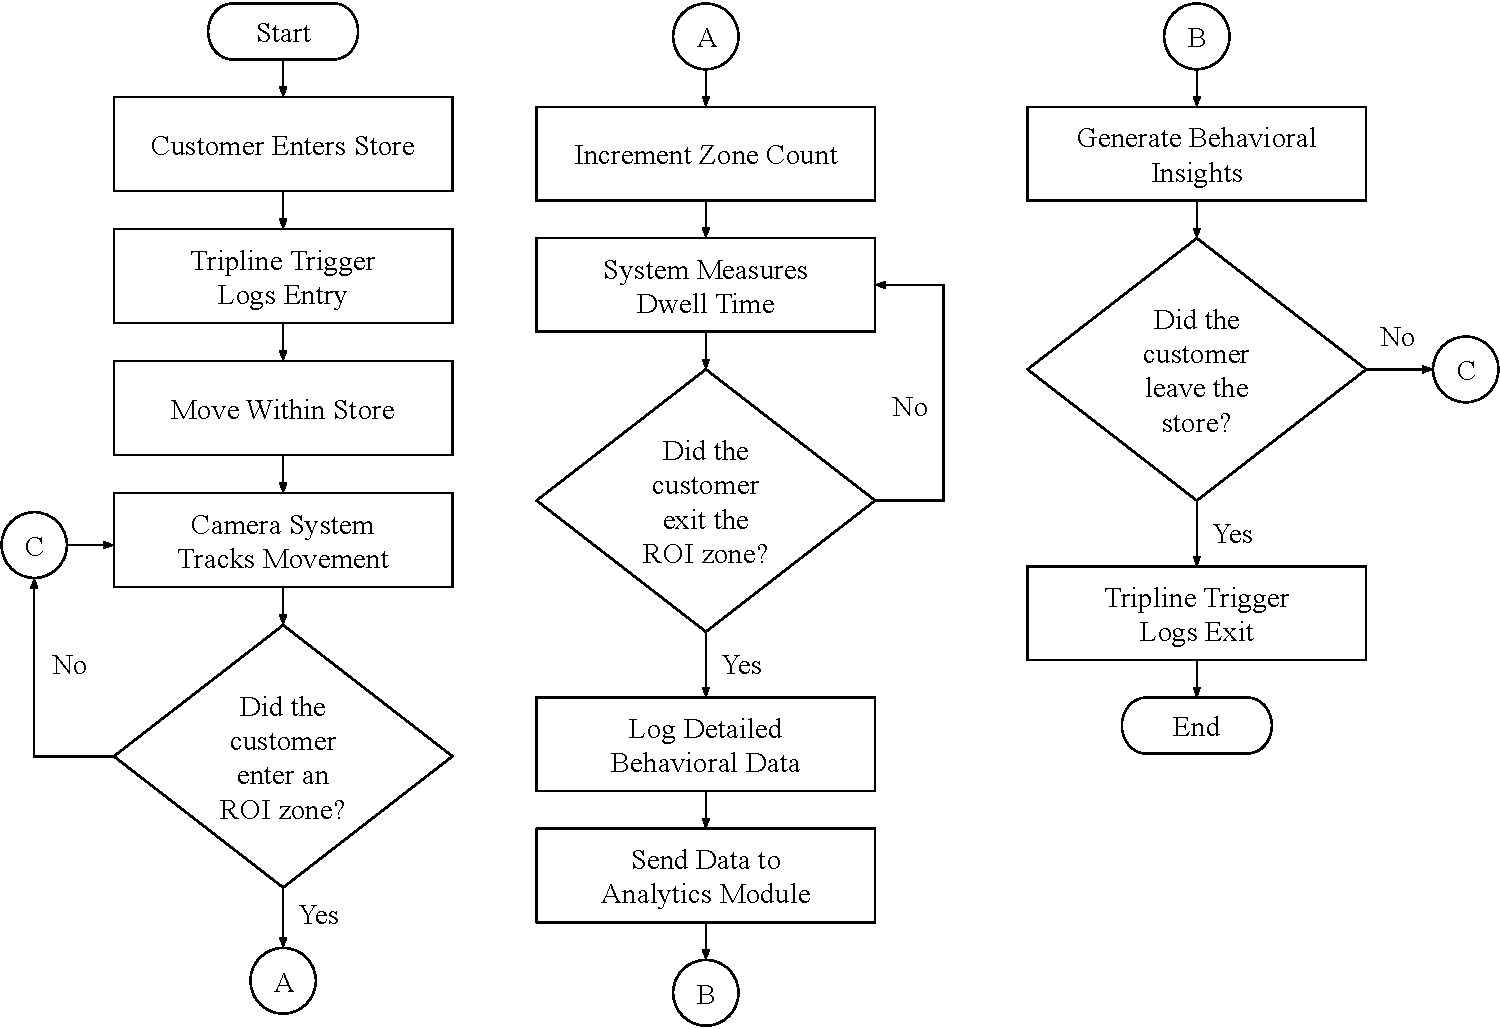
\includegraphics[width=0.75\linewidth]{fig/3.21.pdf}
	\label{fig:3.21}
\end{figure}

As shown in Figure~\ref{fig:3.21}, the system is initialized by connecting to the store’s CCTV cameras, which provide overlapping coverage to minimize blind spots. Once live, YOLOv10 detected individuals in each frame while DeepSORT maintained their unique IDs across angles and occlusions. When a customer entered an ROI, the system triggered a dwell time counter and incremented the zone’s traffic count. This movement data was stored for later analysis and formed the basis for behavioral insights and heat map generation.

\begin{figure}[H]
	\caption[Heat Map Generation Process]{\newline \newline Heat Map Generation Process}
	\centering
	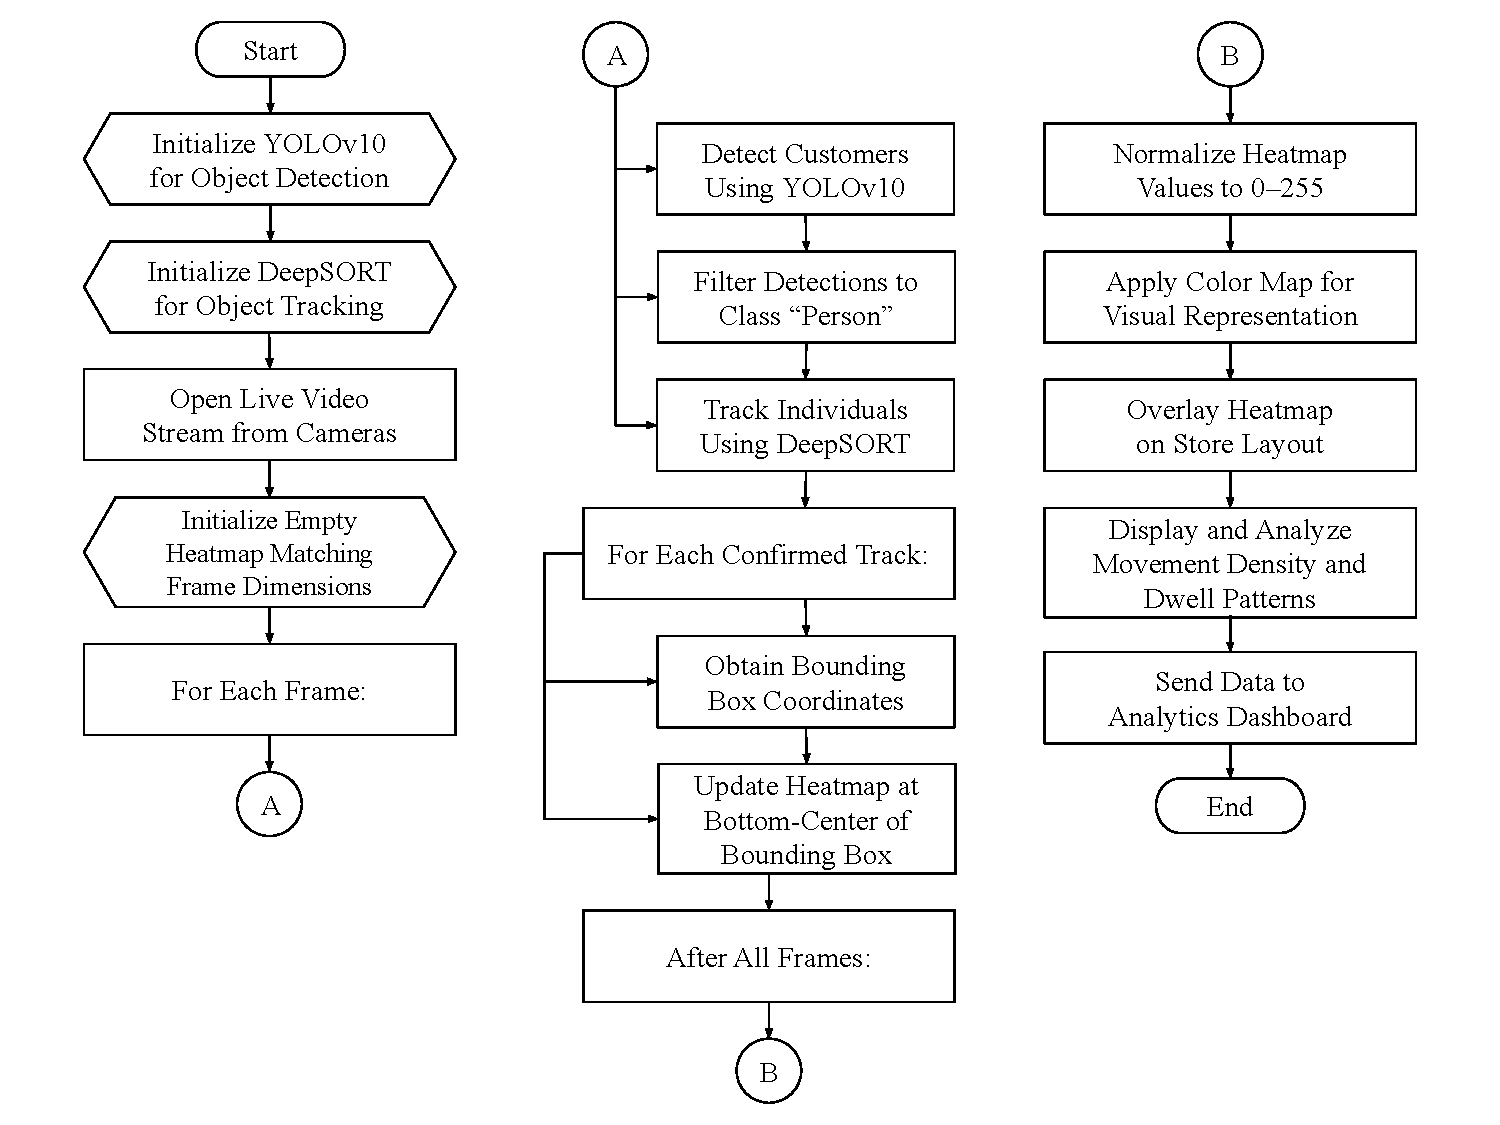
\includegraphics[width=1\linewidth]{figs/3.22.pdf}
	\label{fig:3.22}
\end{figure}

Figure~\ref{fig:3.22} shows how heat maps were created. As video frames were processed, YOLOv10 and DeepSORT tracked each customer's position, marking the bottom-center of their bounding box to map movement within the store. These incremental location updates built a density map, visually representing foot traffic intensity over time. Once processed, the heat map values were normalized, colorized using a gradient, and overlaid on the store layout.

This allowed managers to quickly spot high-engagement areas and underutilized spaces, supporting layout adjustments and marketing strategies. The resulting heat maps and zone metrics were forwarded to the SUBAY dashboard for straightforward interpretation and decision-making.

\subsubsection{Customer Analytics}

The customer behavior analytics module in the SUBAY system was designed to extract actionable insights from tracked movement and interactions within the retail environment. This module operated by capturing surveillance footage from multiple cameras and applying computer vision techniques to interpret customer behavior, specifically, how individuals moved through the store, where they lingered, and which products or zones drew their attention.

As shown in Figure~\ref{fig:3.23}, the system followed a streamlined pipeline that began with detection and tracking using YOLOv10 and DeepSORT. These models ensured consistent identification of individuals across overlapping camera zones, minimizing blind spots and maintaining reliable trajectories. Aggregated movement data, such as zone entries, dwell durations, and path continuity, were then analyzed to produce behavioral metrics.

To inform the final system's user interface and navigation structure, the researchers began by designing the web application using Figma. Wireframes and low-fidelity prototypes were created to map out the application's layout and user flow. This design phase allowed for early visualization of the platform’s core features, including analytics dashboards, navigation menus, and data filters. Iterative refinements were made based on usability and feedback, ensuring that the final system would be accessible and intuitive for retail users with varying technical backgrounds.

\begin{figure}[H]
	\caption[Customer Analytics Process]{\newline \newline Customer Analytics Process}
	\centering
	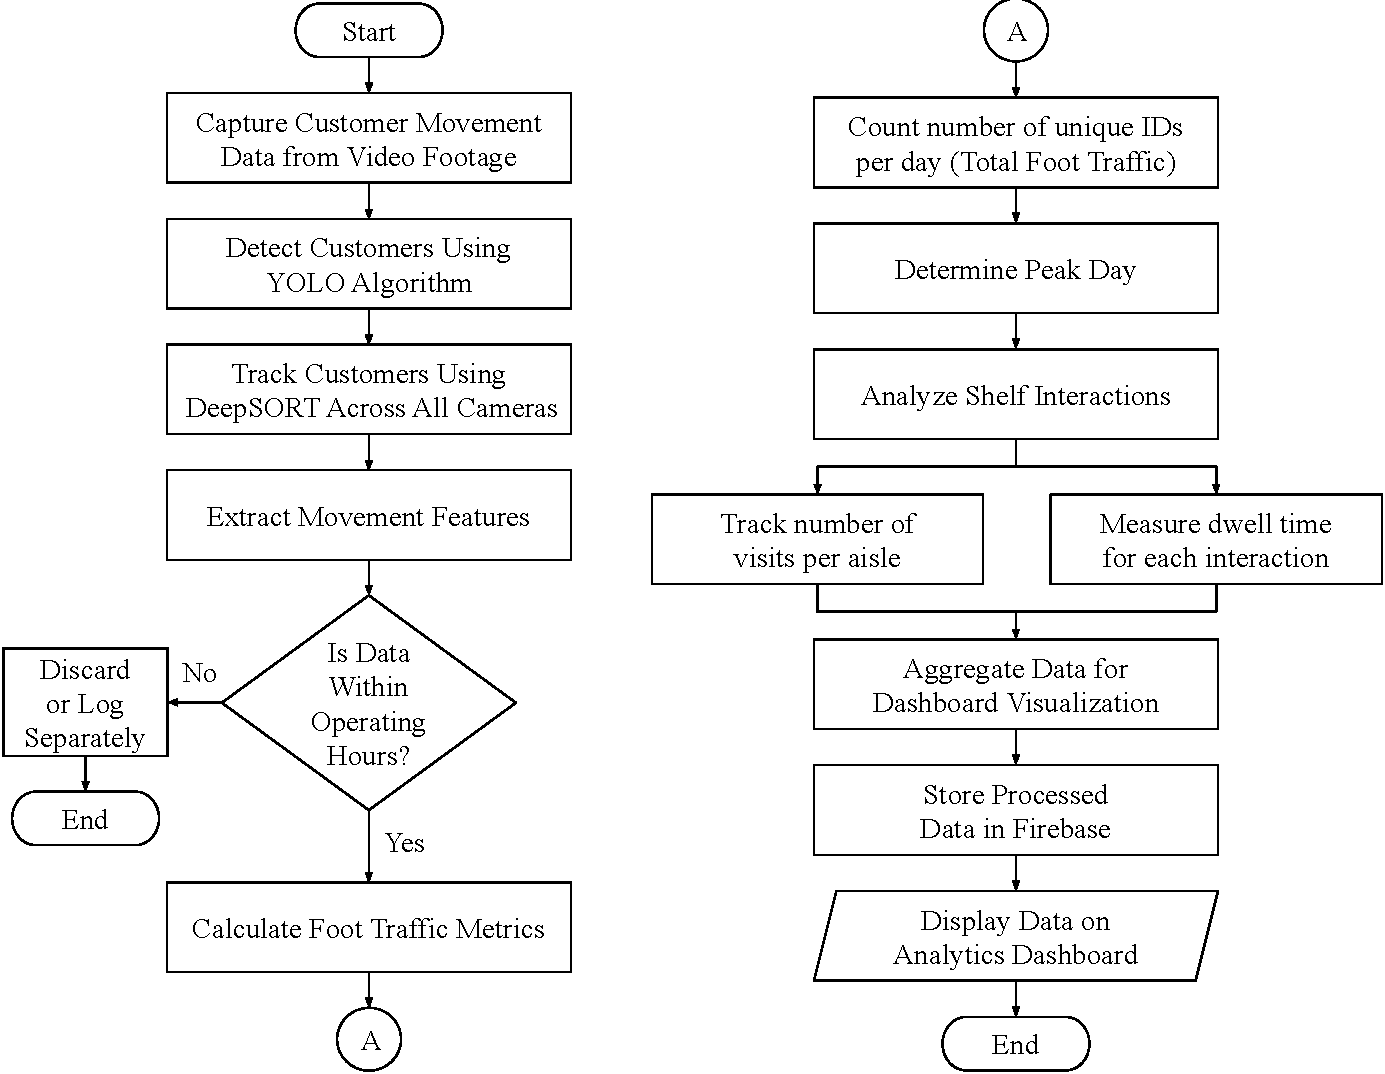
\includegraphics[width=1\linewidth]{fig/3.23.pdf}
	\label{fig:3.23}
\end{figure}

After finalizing the interface design, the researchers implemented the SUBAY web application using modern development technologies. Next.js 15 with TypeScript was used for core application logic, while Tailwind CSS provided a utility-first framework for responsive and customizable styling. ReactJS enabled dynamic, component-based front-end development, enhancing the system’s interactivity and performance. Firebase Cloud Firestore is a real-time NoSQL database on the backend for scalable data storage and retrieval. GitHub was used for version control, supporting collaborative development and secure tracking of code changes. The entire system architecture operated within a Node.js environment, ensuring reliability and responsiveness.

The detection and tracking data collected from video feeds were filtered to exclude activity outside of store hours, maintaining the integrity of the analytics. The system generated key behavioral indicators from this curated data, such as aisle visitation frequency, zone-specific dwell times, heatmap intensity, and peak activity periods.

These insights were visualized through an analytics dashboard that provided interactive charts, graphs, and summary cards. Retail managers could explore metrics such as total daily foot traffic, dwell time distributions, and customer interaction patterns across different store sections. This allowed them to make informed, data-driven decisions about store layout, product placement, and marketing strategy.

Although Live Analytics and Heatmap Overlay pages were also developed to demonstrate the system’s real-time monitoring capabilities, they were excluded from the final deployed version. As outlined in the study’s scope and limitations, only Post-Event Analysis features were retained for deployment. These features allowed the store owner to review and reflect on customer behavior after it occurred, offering valuable insights while preserving system simplicity and privacy. The SUBAY system effectively transformed raw surveillance footage into structured behavioral insights through a robust pipeline of detection, tracking, and analytics delivered via a web application designed to be both functional and user-friendly.

\subsection{Testing \& Evaluation}

To ensure that the SUBAY system met its intended requirements, it underwent a thorough testing and evaluation process. These activities involved the researchers and the intended end user, the retail store owner, to identify any defects, performance issues, or usability concerns that could impact the system’s reliability in a real-world retail environment.

\subsubsection{Testing}

The system was subjected to several levels of testing to verify its functionality and compliance with design specifications. Unit testing was first conducted to validate the performance of individual modules, including camera integration, object detection using YOLO, customer tracking via DeepSORT, and the analytics dashboard. Each module was tested independently to ensure it functioned correctly.

Following this, integration testing evaluated how well the modules worked together, focusing on the seamless data transfer between the detection, tracking, and dashboard components. System testing was then performed to assess the integrated system's operation under real-world conditions, such as customer movement and varying lighting scenarios.

Finally, user acceptance testing (UAT) was conducted with the retail store owner. During this phase, users performed typical tasks while the system’s behavior and their feedback were observed. UAT confirmed the system’s readiness in terms of usability, effectiveness, and alignment with the users’ operational needs.

\subsubsection{Evaluation}

The evaluation process involved both functional and usability testing. A black-box approach was used for functional testing, where different input scenarios were applied without examining the system's internal structure. A customized testing form based on the project’s requirement specifications was used to record whether the system’s outputs aligned with the intended behaviors.

The System Usability Scale (SUS) developed by \cite{Brooke1995} was employed for usability testing. Participants were guided through major system features, such as viewing camera feeds, tracking customer movement, and accessing analytics. Afterward, they completed the SUS questionnaire to assess the system's ease of use, learnability, and user satisfaction. The results provided a quantifiable measure of how intuitive and user-friendly the system was for retail staff. This structured evaluation process refined the SUBAY system to meet technical and end-user expectations, ensuring its readiness for deployment.

\subsubsection{Evaluating Multi-Object Tracking Accuracy and Performance Metrics}

A detailed evaluation of its multi-object tracking performance was conducted to further validate the SUBAY system’s ability to monitor customer movement. The assessment focused on detection accuracy, identity preservation, and tracking precision, using key performance metrics drawn from \cite{Li2023} shown in Table 3.3.

\begin{longtable}[H]{|c|>{\centering\arraybackslash}m{2.2cm}|>{\centering\arraybackslash}m{6.2cm}|>{\centering\arraybackslash}m{3.8cm}|}
	\caption[Evaluation Indicators for Multi-Object Tracking \citep{Li2023}]{\newline \newline Evaluation Indicators for Multi-Object Tracking \citep{Li2023}}\label{tab:mot_metrics}\\
	\hline
	\textbf{Eqn No.} & \textbf{Metric} & \textbf{Formula} & \textbf{Description} \\
	\hline
	\endfirsthead
	
	\multicolumn{4}{c}%
	{\tablename\ \thetable\ -- \textit{Continued from previous page}} \\
	\hline
	\textbf{Eqn \#} & \textbf{Metric} & \textbf{Formula} & \textbf{Description} \\
	\hline
	\endhead
	
	\hline \multicolumn{4}{r}{\textit{Continued on next page}} \\
	\endfoot
	
	\hline
	\endlastfoot
	
	3.1
	& Multiple Object Tracking Accuracy (MOTA) 
	& 
	$
	\text{MOTA} = 1 - \frac{\sum_{t}(FN_t + FP_t + ID\_Swt)}{\sum{t}GT_t}$
	Where:
	\begin{itemize}
		\item $FN_t$: False Negatives at time $t$
		\item $FP_t$: False positives at time $t$
		\item $ID_Sw_t$: ID Switches at time $t$
		\item $GT_t$: Ground Truth Objects at time $t$
	\end{itemize}
	& MOTA was used to measure the overall accuracy of the tracking system by accounting for false positives, false negatives, and ID switches during tracking \citep{Fei2023}. This metric helped determine how well the system avoided tracking errors in practical deployment. \\
	\hline
	
	3.2 
	& Multiple Object Tracking Precision (MOTP) 
	& 
	$
	\text{MOTP} = \frac{\sum{i_t}d{i_t}}{\sum_{t}c_t}
	$
	\newline
	\newline
	Where:
	\begin{itemize}
		\item $d_t$ = 1 - \textit{IOU}, the distance between the ground truth and predicted bounding boxes for object \textit{i} in frame $t$.
		\item $c_t$, the number of matches in frame $t$.
	\end{itemize}
	& MOTP measured how precisely the system localized and tracked individuals. It was calculated based on the Intersection over Union (IoU) of bounding boxes between detected objects and ground truth. This formula measures the average localization precision across all correctly matched pairs in the video sequence \citep{Fei2023}. This metric indicated the system’s spatial tracking precision within the store layout. \\
	\hline
	3.3 
	& Identification Precision (IDP) 
	& $\text{IDP} = \frac{IDTP}{IDTP + IDFP}$
	\newline
	\newline
	Where IDTP and IDFP are the number of valid and false positive IDs, respectively, a high IDP score indicates that customer identities were not incorrectly assigned or merged.
	& IDP evaluated how accurately the system identified and maintained customer identities during tracking. Simply, it is the accuracy of customer ID identification in each bounding box \citep{Fei2023}. \\
	\hline
	3.4 
	& Identification Recall (IDR) 
	& 
	$\text{IDR} = \frac{IDTP}{IDTP + IDFN'}$
	\newline
	\newline
	Where IDFN is the negative ID number, this ensured that the system consistently detected and retained the identities of all customers entering or moving within camera range.
	& IDR assessed how well the system captured and maintained all customer identities across frames. It is the recall rate of customer ID identification in each bounding box \citep{Fei2023}. \\
	\hline
	3.5 
	& Identification F1 Score (IDF1) 
	& 
	$
	\text{IDF1} = \frac{2 \times IDP \times IDR}{IDP + IDR}
	$
	\newline
	\newline
	This metric reflected the system's effectiveness in maintaining consistent identity tracking across multiple frames and camera views.
	& IDF1 represented the harmonic mean between IDP and IDR, offering a balanced measure of identification accuracy. It is the F-value of the customer ID in each bounding box \citep{Fei2023}.\\
\end{longtable}

These tracking performance metrics confirmed that the SUBAY system could reliably track and analyze customer movement patterns even under challenging retail conditions. The results from this evaluation were used to optimize the detection thresholds and improve the synchronization between detection and tracking modules, ultimately contributing to more accurate behavioral analytics and better retail decision-making.

}
	\chapter{RESULTS AND DISCUSSION}
{\baselineskip=2\baselineskip
	
This chapter presents the system implementation results and assesses the extent to which the study’s objectives were accomplished. It covers the performance of the detection, tracking, and counting models, the development of the web-based analytics application, and the evaluation of the system’s accuracy and usability within a real-world retail environment.

\section{Implement Computer Vision Models to Detect, Track, and Count Customers using a Multi-camera Approach.}

This section presents the implementation of the SUBAY system’s core computer vision modules for customer detection, tracking, re-identification, counting, and heat mapping. These modules formed the foundation for the system's ability to monitor customer behavior across multiple store zones. The multi-camera pipeline involved detecting customers in each frame, tracking their movements across time, re-identifying them across different camera views, and aggregating these data points for customer analytics.

\subsection{Customer Detection using YOLOv10}

The customer detection module was the initial step in the SUBAY system’s computer vision pipeline. The YOLOv10x model was utilized for this task due to its balance of detection accuracy and real-time performance. According to \cite{Ultralytics2025}, the YOLOv10x model achieved an Average Precision (APval) of 54.4 at an input size of 640×640, with 160.4 GFLOPs and an inference latency of 10.70 milliseconds, confirming its suitability for deployment in the SUBAY system (see Table 4.1).

\begin{table}[htbp]
	\begin{doublespace}
		\centering
		\caption[Performance Metrics for YOLOv10x \citep{Ultralytics2025}]{\newline \newline Performance Metrics for YOLOv10x \citep{Ultralytics2025}}
		\begin{tabular}{|p{3cm}|p{3cm}|p{2.5cm}|p{2.5cm}|p{2.5cm}|}
			\hline
			\textbf{Model} & \textbf{Input Size} & \textbf{AP\(^\text{val}\)} & \textbf{FLOPs (G)} & \textbf{Latency (ms)} \\
			\hline
			YOLOv10x & 640 & 54.4 & 160.4 & 10.70 \\
			\hline
		\end{tabular}
	\end{doublespace}
	\label{tab:yolov10x}
\end{table}

To validate this model’s real-world capacity to detect customers, the researchers conducted a frame-level analysis using pre-recorded video streams from four different camera angles within a retail store. These views captured a range of conditions, including varying crowd densities, lighting environments, and occlusion scenarios. Figure 4.1 displays sample outputs, illustrating the model's ability to localize customers across zones using bounding boxes.

To manage the large volume of video data, Systematic Random Sampling (SRS) was used to extract representative frames from each camera in the test track. The sampling interval $(k)$ was fixed at 30 based on the track’s frame rate, leaving the sample size $(n)$ as the unknown.

\begin{figure}[H]
	\caption[Sample Detection Outputs using YOLOv10x Across Different Camera Angles]{\newline \newline Sample Detection Outputs using YOLOv10x Across Different Camera Angles}
	\centering
	\includegraphics[width=1\linewidth]{fig/4.1}
	\label{fig:4.1}
\end{figure}

Using the SRS formula, the total number of frames $(N = 13, 888)$ was divided by $k$ ($k$ = number of frames per second of the video) to obtain $n = 463$ frames. Table 4.2 presents the detailed calculations of sampled frames per camera based on this method. Table 4.2 presents the detailed calculations of sampled frames per camera based on this method.


{\doublespacing
	\begin{longtable}{|p{4cm}|p{5cm}|p{5cm}|}
		\caption[Sampling Methodology Overview]{\newline \newline Sampling Methodology Overview} \label{tab:sampling} \\
		\hline
		\textbf{Camera} & \textbf{Total Frames} & \textbf{Sampled Frames} \\
		\hline
		\endfirsthead
		
		\multicolumn{3}{l}{\tablename\ \thetable{} -- \textit{continued from previous page}} \\
		\hline
		\textbf{Camera} & \textbf{Total Frames} & \textbf{Sampled Frames} \\
		\hline
		\endhead
		
		\hline \multicolumn{3}{|r|}{\textit{Continued on next page}} \\ \hline
		\endfoot
		
		\hline
		\endlastfoot
		
		Camera 1 & 3,301 & 110 \\
		\hline
		Camera 2 & 4,199 & 140 \\
		\hline
		Camera 3 & 2,189 & 73 \\
		\hline
		Camera 4 & 4,199 & 140 \\
		\hline
		\textbf{Total} & \textbf{13,888} & \textbf{463} \\
		\hline
		
	\end{longtable}
}


Each sampled frame was then manually annotated to record the following metrics:

\noindent
\begin{itemize}
	\item $\text{True Positives (TP)}$ - correctly detected customers
	\item $\text{False Positives (FP)}$ - non-customers incorrectly identified as customers
	\item $\text{False Negatives (FN)}$ - missed customer detections
	\item $\text{True Negatives (TN)}$ - correctly undetected non-customers (not directly countable)
\end{itemize}

Based on this annotation, the Precision, Recall, and F1 Score were calculated for each camera to assess the model’s performance in practical store conditions (see Table 4.3).

Across all cameras, the model yielded 100\% precision, indicating no false positives after refinement. However, recall values ranged from 89.15\% to 93.06\%, reflecting some missed detections due to occlusion or distance from the camera.

\begin{table}[H]
	\begin{doublespace}
		\centering
		\caption[YOLOv10x Model Accuracy based on the Elements of a Confusion Matrix]{\newline \newline YOLOv10x Model Accuracy based on the Elements of a Confusion Matrix}
		\resizebox{\textwidth}{!}{%
			\begin{tabular}{|p{1.9cm}|p{2.1cm}|p{2.1cm}|p{2.1cm}|p{1.7cm}|p{1.7cm}|p{1.7cm}|p{1.7cm}|}
				\hline
				\textbf{Camera} & \textbf{Total True Positives} & \textbf{Total False Positives} & \textbf{Total False Negatives} & \textbf{Total True Negatives} & \textbf{Precision} & \textbf{Recall} & \textbf{F1 Score}\\
				\hline
				Camera 1 & 411 & 0 & 50 & 20 & 100.00\% & 89.15\% & 94.27\% \\
				\hline
				Camera 2 & 582 & 0 & 61 & 8 & 100.00\% & 90.51\% & 95.02\% \\
				\hline
				Camera 3 & 440 & 0 & 50 & 0 & 100.00\% & 89.80\% & 94.62\% \\
				\hline
				Camera 4 & 738 & 0 & 55 & 0 & 100.00\% & 93.06\% & 96.41\% \\
				\hline
				\textbf{SUM} & \textbf{2171} & \textbf{0} & \textbf{216} & \textbf{28} & \textbf{100.00\%} & \textbf{90.95\%} & \textbf{95.26\%} \\
				\hline
				\textbf{AVERAGE} & \textbf{542.75} & \textbf{0} & \textbf{54} & \textbf{7} & \textbf{100.00\%} & \textbf{90.95\%} & \textbf{95.26\%} \\
				\hline
			\end{tabular}
		}
	\end{doublespace}
\end{table}

Per-camera observations revealed unique detection challenges. Camera 1 experienced detection inconsistencies due to the people visible at the frame’s edge and occasional occlusions caused by shelves or customers entering/exiting the view. Camera 2 was positioned above a densely populated checkout area. Heavy foot traffic, edge-of-frame individuals, and partial occlusion contributed to the model missing some customers. Camera 3 had an ideal angle, avoiding cashier zones and outside interference. It maintained high precision and recall even in slightly occluded scenarios. Camera 4 delivered the most optimal performance. Despite crowd density, it consistently detected customers while lighting conditions were stable.

\begin{figure}[H]
	\caption[YOLOv10 F1 Curve]{\newline \newline YOLOv10 F1 Curve}
	\centering
	\includegraphics[width=0.70\linewidth]{fig/4.2.pdf}
	\label{fig:4.2}
\end{figure}

For the model training and fine-tuning, a dataset comprising 10,635 images of people was integrated into an existing pre-trained model to train a people detection model further using YOLOv10. As shown in the figure, the trained model attained an F1 score of 0.88 at a confidence threshold of 0.80 for the "person" class. This performance suggests that the model effectively detects individuals in videos with high precision and recall at the specified confidence level.

\subsection{Customer Tracking using DeepSORT}

After detecting customers, the system used the DeepSORT algorithm to assign and maintain unique tracking IDs across consecutive video frames and overlapping store zones. While effective in many scenarios, DeepSORT faced difficulty maintaining consistent IDs across all four cameras. ID switches occurred during transitions between views, in poor lighting conditions, or when individuals were partially obscured. These issues were more common near frame edges or in crowded areas. However, DeepSORT often re-identified individuals after temporary disappearance, particularly when they returned to the center of the frame. Figure~\ref{fig:4.3} shows a sample frame with consistent and inconsistent ID assignments during tracking.

\begin{figure}[H]
	\caption[Consistent and Inconsistent ID Assignments during DeepSORT Tracking]{\newline \newline Consistent and Inconsistent ID Assignments during DeepSORT Tracking}	
	\centering
	\includegraphics[width=1\linewidth]{fig/4.3.pdf}
	\label{fig:4.3}
\end{figure}

To evaluate DeepSORT's performance, a set of designated video test clips was extracted from various in-store conditions. Table 4.4 summarizes the tracking outcomes using key performance indicators:

\textit{- Total Tracked Customers} refers to the number of unique individuals detected and monitored throughout a test sequence.

\textit{- ID Switches} capture instances where DeepSORT mistakenly assigned a different ID to the same person, indicating a lapse in identity preservation.

\textit{- Re-ID Success Rate (\%)} measures the algorithm's ability to successfully re-identify individuals after temporary occlusion or after exiting and re-entering a frame. It is calculated as:

\begin{equation}
	\text{Re-ID Success Rate} = (\frac{\textit{Total Tracked Customers - ID Switches}}{\textit{Total Tracked Customers}}) \times 100
\end{equation}
\myequation{Re-ID Success Rate}

This metric conceptually aligns with the Rank-1 Accuracy used in person re-identification benchmarks, where a correct match is counted if the correct identity appears as the top-ranked result \citep{Zheng2015}. While simplified, this formulation remains effective for evaluating practical system-level performance in real-world environments.

The performance results of DeepSORT across the different in-store scenarios highlighted its strengths and limitations. The algorithm successfully tracked many customers in regular traffic aisles, but 45 ID switches led to a moderate Re-ID success rate of 53\%.

\begin{table}[H]
	\centering
	\caption[Customer Tracking Performance Across Different Retail Scenarios]{\newline \newline Customer Tracking Performance Across Different Retail Scenarios}
	\begin{tabular}{|p{1.5cm}|p{1.5cm}|p{1.5cm}|p{1.8cm}|p{3.5cm}|}
		\hline
		\textbf{Scenario} & \textbf{Total Tracked Customers} & \textbf{ID Switches} & \textbf{Re-ID Success Rate (\%)} & \textbf{Notes:} \\
		\hline
		Normal traffic aisle & 96 & 45 & 53\% & Moderate foot traffic with occasional occlusion \\
		\hline
		Crowded aisle & 32 & 17 & 47\% & High density, overlapping paths, and frame-edge exits \\
		\hline
		Occlusion-heavy zones & 24 & 18 & 25\% & Frequent obstruction by shelves, other customers, or fixtures \\
		\hline
		Camera transition zones & 21 & 11 & 48\% & Movement across overlapping fields of view and lighting changes \\
		\hline
	\end{tabular}
	\label{tab:customer_tracking}
\end{table}

Performance declined in crowded aisles and occlusion-heavy zones, where overlapping paths and frequent obstructions caused more ID mismatches, resulting in lower Re-ID rates of 47\% and 25\%, respectively. The camera transition zones posed additional challenges due to changes in angles and lighting, achieving a Re-ID success rate of 48\%. These results indicate that while DeepSORT can work in less complex conditions, its identity consistency degrades in visually dynamic or cluttered environments, an essential consideration for improving system robustness.

\subsection{Re-Identification with Omni-Scale Network}

To address DeepSORT’s limitations in maintaining consistent identity tracking across multiple overlapping camera frames, the system incorporated a Person Re-Identification (Re-ID) model. This model aimed to enhance cross-view identity continuity by re-matching customers based on visual features, even when tracked IDs were disrupted due to occlusion, crowding, or camera transitions.

The Re-ID model was trained using annotated image datasets containing customer appearances across multiple store cameras. Feature embeddings were extracted and processed using the Omni-Scale Network (OSNet), a deep learning architecture known for its robust performance in cross-view appearance matching as discussed in the previous chapter.

\begin{figure}[H]
	\caption[Sample Customers in the Re-identification Dataset Across Different Camera Views]{\newline \newline Sample Customers in the Re-identification Dataset Across Different Camera Views}
	\centering
	\includegraphics[width=0.75\linewidth]{fig/4.4.pdf}
	\label{fig:4.4}
\end{figure}

Figure~\ref{fig:4.4} presents sample subjects from the training dataset, arranged in camera sequence from left to right: Camera 02, Camera 05, Camera 03, and Camera 09.

After training, the model was evaluated using a test dataset, achieving an accuracy of 75.48\%, a precision of 73.70\%, a recall of 70.70\%, and an F1-score of 72.17\% as summarized in Table 4.5. These metrics confirmed the model’s reliability in controlled testing environments, validating its integration into the multi-camera tracking pipeline for retail analytics.

\begin{table}[htbp]
	\begin{doublespace}
		\centering
		\caption[Re-Identification Model Training Results]{\newline \newline Re-Identification Model Training Results}
		\begin{tabular}{|c|c|c|c|}
			\hline
			\textbf{Accuracy} & \textbf{Precision} & \textbf{Recall} & \textbf{F1-Score} \\
			\hline
			75.48 & 73.70 & 70.70 & 72.17 \\
			\hline
		\end{tabular}
	\end{doublespace}
\end{table}

The trained Re-ID model was tested on a video sequence featuring customer movements across overlapping store zones to assess its applicability in real-world conditions. The aim was to evaluate how the model responded to typical challenges such as occlusions, dynamic lighting, and varying subject positions.

Figure~\ref{fig:4.5} shows Case A, in which the same individual was correctly identified across all four camera views. This ideal scenario occurred under good lighting and centered framing, confirming optimal model behavior.

\begin{figure}[H]
	\caption[Re-Identification Case A: Perfect Re-Identification Across All Camera Views]{\newline \newline Re-Identification Case A: Perfect Re-Identification Across All Camera Views}
	\centering
	\includegraphics[width=1\linewidth]{fig/4.5.pdf}
	\label{fig:4.5}
\end{figure}

Figure~\ref{fig:4.6} presents Case B, a near-complete match disrupted by heavy shelf occlusion in the fourth view. The subject was successfully re-identified in the first three views but was missed in the obstructed one.

\begin{figure}[H]
	\caption[Re-Identification Case B: Near-complete Re-Identification Affected by Shelf Occlusion]{\newline \newline Re-Identification Case B: Near-complete Re-Identification Affected by Shelf Occlusion}
	\centering
	\includegraphics[width=0.75\linewidth]{fig/4.6.pdf}
	\label{fig:4.6}
\end{figure}

Case C (Figure~\ref{fig:4.7}) represented a more difficult scenario. The model correctly re-identified the subject in only two of the four views. The remaining views experienced ID switches due to occlusion, off-angle appearances, and varied lighting conditions commonly encountered in operational environments.

While OSNet significantly enhanced identity retention across overlapping camera views, its effectiveness was influenced by external factors. The system performed well in clear, centered, and well-lit frames, but struggled with occlusion, off-angle shots, and inconsistent illumination. These findings underscore the need for improved scene normalization techniques or camera placements that reduce ambiguity in customer visibility.

\begin{figure}[H]
	\caption[Re-Identification Case C: Partial Re-Identification with ID Switches in Overlapping Views]{\newline \newline Re-Identification Case C: Partial Re-Identification with ID Switches in Overlapping Views}
	\centering
	\includegraphics[width=1\linewidth]{fig/4.7.pdf}
	\label{fig:4.7}
\end{figure}

Despite these limitations, the OSNet-based Re-ID model played a critical role in bridging the identity gaps that DeepSORT alone could not resolve, ultimately strengthening the accuracy of the system's behavioral analytics in complex retail environments.

\subsection{Customer Counting Mechanisms}
The customer counting module combined YOLOv10, DeepSORT, and tripline analysis to estimate customer entries and monitor presence across designated store zones. Upon booting the system, the customers it “sees” were assigned unique tracking IDs. An ROI tripline is also virtually placed at the store entrance on one camera frame. This approach prevented double-counting by ensuring each individual was only counted once per entry event. Figure~\ref{fig:4.8} presents a sample frame showing the total customer count and the current count in the store.

\begin{figure}[H]
	\caption[Sample Frame Showing Total Customer Count and Current Count in the Store]{\newline \newline Sample Frame Showing Total Customer Count and Current Count in the Store}
	\centering
	\includegraphics[width=0.75\linewidth]{fig/4.8.pdf}
	\label{fig:4.8}
\end{figure}

Once detected and assigned a unique ID, the system continuously monitored the customer’s movement and logged their presence duration. This enabled the calculation of individual dwell time and overall customer traffic within the monitored space. A summary of results from a test track is provided in Table 4.6.

Total Foot Traffic refers to the number of unique individuals detected by the system, assigned a unique ID, and successfully tracked during the test period. Total Customer Dwell Time represented the cumulative duration, in both seconds and minutes, that all tracked customers spent in the store zone. Average Dwell Time was computed by dividing the total dwell time by the total foot traffic, indicating how long a typical customer remained in the observed area.

\begin{table}[H]
	\begin{doublespace}
		\centering
		\caption[Summary of Customer Count and Dwell Time Based on Test Track]{\newline \newline Summary of Customer Count and Dwell Time Based on Test Track}
		\resizebox{\textwidth}{!}{%
			\begin{tabular}{|p{2.5cm}|p{2.5cm}|p{2.5cm}|p{2.5cm}|p{2cm}|p{2cm}|p{2cm}|}
				\hline
				\textbf{Total Foot Traffic} & \textbf{Total Customer Dwell Time (secs)} & \textbf{Total Customer Dwell Time (min)} & \textbf{Average Dwell Time (secs)} & \textbf{Average Dwell Time (mins)} \\
				\hline
				33 & 4,877.17 & 81.29 & 147.79 & 2.46 \\
				\hline
			\end{tabular}
		}
	\end{doublespace}
\end{table}

These results demonstrated the system’s ability to accurately count foot traffic and analyze customer engagement time. Such data can inform critical operational decisions, including staff allocation, store layout adjustments, and targeted marketing efforts. The ability to measure both frequency and duration of customer visits provided actionable insights for enhancing in-store experiences and improving overall retail performance.

\subsection{Zone-Based Analytics and Heat Map Visualization}

The system implemented zone-based counting and heat map visualization to generate deeper insights into customer movements and behavior. Key store areas, such as aisles and product displays, were designated as Regions of Interest (ROIs) to monitor and quantify customer presence and movement. Aggregated movement data across these zones enabled the generation of heat maps that visually represented both dwell time and customer density. Figure~\ref{fig:4.9} shows a sample heat map overlay that visualizes the intensity of customer activity.

Figure~\ref{fig:4.9} presents a visual overlay combining camera footage with a dynamic heatmap. This visualization serves as an analytical tool to monitor customer movement, density, and dwell time within distinct product zones of the store. Each aisle holds different kinds of products like Aisle 1 with Body and Bath Products, Aisle 2 with Face and Hair Care Products, Aisle 3 with Cosmetics, Aisle 4 with Assorted Home Essentials, Aisle 5 with Kitchenwares, and Aisle 6 with Home Products. Warmer areas on the heatmap indicate zones with heavier foot traffic or longer dwell time, while cooler areas suggest less interaction. This allows store managers to assess which product categories attract more attention, optimize layout design, and make data-driven decisions on product placement or promotions.

\begin{figure}[H]
	\caption[Heatmap Overlay Indicating Customer Density and Dwell Time]{\newline \newline Heatmap Overlay Indicating Customer Density and Dwell Time}
	\centering
	\includegraphics[width=0.75\linewidth]{fig/4.9.pdf}
	\label{fig:4.9}
\end{figure}

\subsection{Accuracy of System-Generated Tracking Compared to Manual Observation}

To evaluate the effectiveness of the SUBAY system in detecting and tracking customers within a retail environment, a comparative analysis was performed between manual annotations and system-generated outputs. This assessment aimed to determine how closely the system could replicate the accuracy of human observation when identifying customer locations over time.

\begin{figure}[H]
	\caption[Intersection over Union (IoU) per Frame]{\newline \newline Intersection over Union (IoU) per Frame}
	\centering
	\includegraphics[width=0.85\linewidth]{fig/4.10.pdf}
	\label{fig:4.10}
\end{figure}

Figure~\ref{fig:4.10} shows two line graphs that illustrate this comparison using data collected from over 5,000 frames of synchronized video footage. The first graph at the top displays the level of overlap between the bounding boxes drawn manually (ground truth) and those generated by the system. This overlap is expressed as a value between 0 and 1, where 1 represents perfect alignment. The graph shows that the overlap remained consistently high throughout the frames, with most values hovering around 0.9 or above. The average overlap achieved was approximately 0.9190, suggesting that the system was highly accurate in placing detection boxes around customers nearly the same way a human would.

\begin{figure}[H]
	\caption[Center Distance per Frame]{\newline \newline Center Distance per Frame}
	\centering
	\includegraphics[width=0.85\linewidth]{fig/4.11.pdf}
	\label{fig:4.11}
\end{figure}

Figure~\ref{fig:4.11} illustrates the distance, measured in pixels, between the centers of the manually and system-drawn boxes for each frame. Lower values in this graph represent closer agreement between the two. The average distance recorded was 6.71 pixels, which is considered minimal and indicates that even when there were slight differences in the size or shape of the boxes, the system still correctly pinpointed the customer's general location.

These two visualizations demonstrate that the SUBAY system could precisely track customer movement across frames. The consistently high overlap and low center distance highlight the reliability of the system’s detection accuracy, closely matching manual observation. This level of performance is crucial for ensuring the validity of customer behavior analytics derived from system-tracked data, such as counting foot traffic, analyzing dwell time, and generating heat maps. The close agreement between manual and automated tracking further supports the system’s readiness for deployment in real-world retail settings where accurate customer insights are essential.

\subsection{Evaluation of Multi-Object Tracking Accuracy and Performance Metrics}

A performance analysis was conducted to evaluate the object tracking capabilities of the SUBAY system using a unified tracking configuration. This setup employed YOLOv10 integrated with DeepSORT and enhanced by the Omni-Scale Re-Identification (Re-ID) module. The system’s effectiveness is visualized using widely accepted multi-object tracking evaluation indicators, as outlined by the studies of \cite{Amosa2023}, \cite{Fei2023}, and \cite{Li2023}. These metrics include: Multiple Object Tracking Accuracy (MOTA), Multiple Object Tracking Precision (MOTP), Identification Precision (IDP), Identification Recall (IDR), and the Identification F1 Score (IDF1).

\begin{figure}[H]
	\caption[Performance of the YOLOv10 + DeepSORT + Omni-Scale Re-ID System]{\newline \newline Performance of the YOLOv10 + DeepSORT + Omni-Scale Re-ID System}
	\centering
	\includegraphics[width=0.85\linewidth]{fig/4.12.pdf}
	\label{fig:4.12}
\end{figure}

Figure~\ref{fig:4.12} presented in this subsection, illustrates the performance of the YOLOv10 + DeepSORT + Omni-Scale Re-ID system across five key multi-object tracking evaluation metrics: MOTA, MOTP, IDP, IDR, and IDF1. Each score is displayed as a point along the vertical axis, ranging from 0 to 1, where higher values indicate better performance.

Starting with MOTA (Multiple Object Tracking Accuracy), the system achieves a score of 0.602, indicating solid overall tracking performance. This metric encapsulates false positives, false negatives, and identity switches. Hence, a score above 0.6 demonstrates the system's capability to track multiple individuals with reasonable consistency, especially in complex, real-world environments involving multiple cameras, occlusions, and identity changes.

The MOTP (Multiple Object Tracking Precision) is notably high at 0.910, showcasing the system’s ability to localize targets accurately within each frame. This score reflects the spatial precision of bounding boxes, suggesting that YOLOv10 detections are tightly aligned with ground-truth person locations. This is crucial for precise and reliable visualization in surveillance or retail analytics.

For Identification Precision (IDP), the system records a score of 0.577, reflecting the proportion of correctly assigned identities among all identity predictions. While this value is moderate, it underscores the inherent complexity of re-identification in a multi-camera system, especially one involving four camera views. IDP is only rewarded in this setup when the same individual is consistently recognized across all four camera streams within the same frame instance (see figure~\ref{fig:4.5}). This constraint introduces evaluation challenges: if the system requires several frames to accumulate enough visual information to match a person across views confidently, say, identifying a person correctly only by the fourth frame, then the earlier mismatches reduce the precision score. In this instance, a correct identification occurring only once across four frames would contribute just 25\% (1/4) to the IDP metric, even if the system eventually makes the right call. As a result, the IDP score may underrepresent the system’s true long-term identity tracking capability, especially when appearance changes, occlusions, or view transitions delay accurate matching across all camera views.

However, in Identification Recall (IDR), a measure of how many true identities were correctly retrieved, the system is slightly higher at 0.612, meaning it is relatively better at retrieving the correct identities among the ground-truth individuals. This implies that the Re-ID module, based on Omni-Scale feature extraction, effectively matches many individuals across camera views, even if not all identity assignments are precise.

Finally, the IDF1 score, which combines a balanced harmonic mean of IDP and IDR, resulted in 0.595, highlighting the system’s overall identity tracking performance. This value reflects a reasonable balance between correct identity assignment and retrieval. It also demonstrates the Re-ID model’s ability to preserve identity over time and across camera views with moderate success.

These results highlight the effectiveness of combining Omni-Scale Re-ID with YOLOv10 + DeepSORT for multi-camera person tracking. The notably high MOTP underscores the system’s strong detection accuracy, while the MOTA and IDF1 scores indicate reliable tracking performance and identity consistency even in complex, multi-view environments. Despite some limitations in identity precision, particularly in early cross-camera associations, the system demonstrates considerable potential for real-world deployments, especially in domains like retail analytics, intelligent surveillance, and multi-camera monitoring, where sustained identity tracking across diverse scenes is essential.

\section{Develop a Web Application for Data Visualization and Customer Analytics from the Results of the Detection, Tracking, and Customer Counting Models.}

A responsive and user-friendly web application was then developed to serve as the main platform for presenting the outputs of the detection, tracking, and customer counting models. Using Firebase for backend support, the system provided real-time updates and organized the visualized data through interactive dashboards and charts. Each page of the application was structured to help users interpret customer behavior more effectively, with features ranging from secure login and live analytics to post-event analysis and insight generation.

\subsection{User Access and Navigation Structure}

The web application consisted of several core pages and functionalities. Upon launching the system, users were greeted with the Welcome Page. As shown in Figure~\ref{fig:4.13}, the Welcome Page featured the (1) SUBAY Logo positioned prominently at the center to establish branding, the (2) Thesis Title displayed adjacent to it to introduce the project, and the (3) Login Button located beneath the title, allowing users to proceed to the secure login page.

\begin{figure}[H]
	\caption[Welcome Page]{\newline \newline Welcome Page}
	\centering
	\includegraphics[width=1\linewidth]{fig/4.13.pdf}
	\label{fig:4.13}
\end{figure}

The system then directed users to the Login Page. Figure~\ref{fig:4.14} depicts the Login Page layout, which included several critical functional elements: the (1) Log in Box where all credentials were entered, the (2) Log in Title positioned at the top to guide users, the (3) Email Credential input field, and the (4) Password Credential input field essential for authentication. Below the input fields, the (5) Log in Button was provided to initiate the login process, and below the form, the (6) Copyright Statement acknowledged the work's intellectual property.

\begin{figure}[H]
	\caption[Login Page]{\newline \newline Login Page}
	\centering
	\includegraphics[width=1\linewidth]{fig/4.14.pdf}
	\label{fig:4.14}
\end{figure}

After successful authentication, users were redirected to the Dashboard Page, which served as the central hub of the SUBAY system. As shown in Figure 4.15, the dashboard offered streamlined access to all major features and presented a comprehensive overview of system insights. On the left side, the (1) Sidebar Menu provided navigational access to key modules such as the (3) Home Page, (4) Live Analytics Page, (5) Heatmapping Page, (6) Post Analytics Page, (7) Insights Page, and (8) About Page. Users could also minimize the sidebar using the (2) Collapse Sidebar Button to maximize screen space.

\begin{figure}[H]
	\caption[Dashboard Page]{\newline \newline Dashboard Page}
	\centering
	\includegraphics[width=1\linewidth]{fig/4.15.pdf}
	\label{fig:4.15}
\end{figure}

At the top of the interface, the (9) Topbar / Title indicated the current section being viewed, while the (10) User Toggle Button allowed access to account settings and logout functionality. Within the main dashboard view, direct navigation was provided through quick-access buttons, including the (11) Direct Route to Live Analytics Page, (12) Heatmapping Page, (13) Post Analysis Page, and (14) Insights Page.

The dashboard also displayed a variety of interactive components. The (15) Camera Feed Card previewed video input from active feeds, while the (17) Live Cameras Available Card and (18) Available Dates Card helped users identify currently active cameras and available analytics data. Visual summaries were presented through the (22) Total Foot Traffic Pie Chart, (24) Average Dwell Time Line Chart, and (25) Aisle-Based Foot Traffic and Dwell Time Bar Chart, providing clear overviews of behavioral patterns.

To highlight key insights at a glance, the dashboard featured the (19) Peak Visit Aisle Card and (20) Peak Dwell Aisle Card, showing which zones had the highest foot traffic and longest dwell time, respectively. The (21) Live Analysis Card displayed dynamic tracking metrics. Users could also access deeper analysis via the (16) Open Live Analytics Page and the (23) Open to Insights Page options. Finally, a (26) Theme Toggle allowed users to switch between dark and light modes for a more personalized viewing experience.

\subsection{Real-time Analysis}

\begin{figure}[H]
	\caption[Live Analytics Page]{\newline \newline Live Analytics Page}
	\centering
	\includegraphics[width=0.80\linewidth]{fig/4.16.pdf}
	\label{fig:4.16}
\end{figure}

The Live Analytics Page, displayed in Figure~\ref{fig:4.16}, demonstrated real-time monitoring capabilities of the system. The page consisted of several key components: the (1) Live Analytics Feed, presenting a real-time view of detected customers, the (2) Live Total Customer Count summarizing the cumulative foot traffic, the (3) Live Current Customers Count showing the active number of customers within the store, the (4) Live Total Aisle Visits tracking customer movement across zones, and the (5) Live Average Dwell Time (in seconds) providing immediate insight into customer engagement duration.

\begin{figure}[H]
	\caption[Heat Mapping Page]{\newline \newline Heat Mapping Page}
	\centering
	\includegraphics[width=1\linewidth]{fig/4.17.pdf}
	\label{fig:4.17}
\end{figure}

The system also featured a Heat Mapping Page for spatial behavior visualization. As shown in Figure~\ref{fig:4.17}, the Heat Mapping Page consisted of the (1) Camera Feed displaying the active surveillance view and the (2) Heat map Overlay applied atop the feed, illustrating customer density and movement patterns with color gradients.

\subsection{Post-Event Analysis}

\begin{figure}[H]
	\caption[Post Analytics Page]{\newline \newline Post Analytics Page}
	\centering
	\includegraphics[width=1\linewidth]{fig/4.18.pdf}
	\label{fig:4.18}
\end{figure}

The Post Analytics Page enables users to analyze store performance after events. Figure 4.18 shows the Post Analytics Page, which incorporated the following elements: (1) Customer and Zone-based Counting to contrast movement trends, (2) Heat Map Overlay for post-event spatial distribution, (3) Total Foot Traffic metrics, (4) Average Dwell Time measurements, and (5) Aisle-Based Foot Traffic and Dwell Time distributions, providing actionable insights on customer interactions with different store zones.

\begin{figure}[H]
	\caption[Insights Page]{\newline \newline Insights Page}
	\centering
	\includegraphics[width=1\linewidth]{fig/4.19.pdf}
	\label{fig:4.19}
\end{figure}

As presented in Figure~\ref{fig:4.19}, the Insights Page consolidated analytical findings into strategic recommendations. Functional elements included the peak metrics cards, (1) Aisle with the highest visit indicator, and (2) Aisle with the highest dwell time indicator to highlight critical engagement areas. Three charts were provided with user interaction options: the (3) Total Foot Traffic Pie Chart with an integrated Date Range Picker and Expand Button, the (4) Average Dwell Time per Aisle Line Chart with similar interactive controls, and the (5) Aisle-Based Foot Traffic and Dwell Time Bar Chart. Additionally, the (6) Generate Insights Button was incorporated to automate the generation of narrative summaries based on the analyzed data.

\subsection{Insight Generation}
One of the significant outcomes of the system's development was the integration of an automated insight generation module, as outlined in the Activity Diagram for Insight Generation. This module processed the aggregated outputs from customer detection, tracking, and counting to derive high-level behavioral analytics. Through this workflow, the system transformed raw customer movement data into concise summaries, logical conclusions, and actionable recommendations designed to support informed decision-making by store managers.

\begin{figure}[H]
	\caption[Insight Generation]{\newline \newline Insight Generation}
	\centering
	\includegraphics[width=0.8\linewidth]{fig/4.20.pdf}
	\label{fig:4.20}
\end{figure}

The Insight Generation functionality was accessed through the Insights Page of the web application, as shown in Figure~\ref{fig:4.20}. The system automatically computed several key performance metrics after collecting detection and tracking outputs over a monitoring period. These included:

\noindent - Total Foot Traffic: The number of unique entries during the monitored period.

\noindent - Peak Day Analysis: Identifying the day with the most customer entries.

\noindent - Zone-Based Foot Traffic: Highlighting which aisle attracted the most traffic.

\noindent - Zone-Based Dwell Time: Measuring where customers lingered the longest.

\noindent - Average Dwell Time: Calculated across all store zones to gauge overall engagement.

\begin{figure}[H]
	\caption[Sample Generated Analytics Report Output]{\newline \newline Sample Generated Analytics Report Output}
	\centering
	\includegraphics[width=1\linewidth]{fig/4.21.pdf}
	\label{fig:4.21}
\end{figure}

Figure~\ref{fig:4.21} presents the sample downloadable generated analytics report output. These computations were processed programmatically through the web application's backend, where pieChartData and barChartData were analyzed to derive summarized figures. Specific computations included summing total entries, calculating total traffic per zone percentages, identifying top-performing and underperforming aisles, and determining average and peak dwell times.

These values were then evaluated against industry performance thresholds. According to BPlanAI (2025) and \cite{CountTrack2025}, retail stores with beauty items typically see 50–80 daily visitors, and healthy customer dwell time ranges between 10 and 20 minutes. Using this guidance, the system programmatically flagged the store as performing well since:

\noindent - The Average Daily Foot Traffic was 51.80, well above the minimum benchmark.

\noindent - Average Customer Dwell Time was 11.31 minutes, indicating sustained engagement.

The results were automatically compiled into a downloadable Retail Insight Report, which presented the findings in a user-friendly format, such as in the sample report shown in Figure 4.22.

\noindent - The total foot traffic recorded during the monitoring period was 259 entries.

\noindent - The peak day was April 13, 2025, with 78 entries (30.12\% of all traffic).

\noindent - Aisle B emerged as the zone with the highest foot traffic, accounting for 30 recorded entries (39.38\%).

\noindent - Aisle A was highlighted as the zone with the longest total dwell time, totaling 105.38 minutes.

\noindent - The total customer dwell time across all zones is 339.3 minutes, and the average dwell time across all zones is 11.31 minutes, indicating a healthy level of customer engagement.

Beyond numerical reporting, the system generated conclusions based on pre-established logic conditions.

\begin{figure}[H]
	\caption[Sample Report’s Results]{\newline \newline Sample Report’s Results}
	\centering
	\includegraphics[width=1\linewidth]{fig/4.22.pdf}
	\label{fig:4.22}
\end{figure}

In Figure~\ref{fig:4.23}, the system concluded, "The store is performing well, recording an average of 51.80 daily foot traffic with an average dwell time of 11.31 minutes.” This indicates healthy foot traffic and meaningful customer engagement.

\begin{figure}[H]
	\caption[Sample Report’s Conclusions]{\newline \newline Sample Report’s Conclusions}
	\centering
	\includegraphics[width=1\linewidth]{fig/4.23}
	\label{fig:4.23}
\end{figure}

Furthermore, the recommendations were automatically produced based on the computed insights exemplified in Figure~\ref{fig:4.24}. These included:

\noindent - Leverage Top-Performing Aisles: Leverage the success of Aisle B, which accounted for 39.38\% of all foot traffic. Place new or high-margin products here to maximize visibility and drive sales.

\noindent - Replicate the Success of Long-Dwell Aisles: Study the characteristics of Aisle A, where customers spent an average of 1.44 minutes. Identify what makes this zone engaging, such as layout, product type, or sensory elements, and replicate it in other underperforming zones.

\noindent - Elevate Low-Performers Strategically: While overall performance is strong, consider improving the layout or visual appeal of less-visited aisles like Aisle E. This will balance store flow and reduce congestion in high-traffic zones.

\noindent - Continuous Monitoring: Establish a routine for weekly or monthly monitoring. Use these trends to make dynamic layout decisions and prepare promotions aligned with peak traffic patterns (e.g., around April 13, 2025).

The automated insight generation module of SUBAY successfully translated customer behavior metrics into scientifically derived and strategically valuable insights. Combining visualized data with coded logic referencing industry benchmarks empowered store managers to assess engagement performance quickly, identify top and underperforming zones, strategically place products, optimize layouts, and adapt marketing efforts to customer behavior. This section validated how SUBAY’s analytics engine supported evidence-based retail decision-making, providing data and interpretation tailored to business needs.

\begin{figure}[H]
	\caption[Sample Report’s Recommendations]{\newline \newline Sample Report’s Recommendations}
	\centering
	\includegraphics[width=0.75\linewidth]{fig/4.24.pdf}
	\label{fig:4.24}
\end{figure}

\section{Evaluate the Performance and Usability of the Multi-camera Object Detection System.}
This section outlines the results obtained from testing and evaluating the SUBAY system after its implementation. It includes the system's Zone-based Foot Traffic and Dwell Time Count results and the outcomes of functional and usability testing from the perspective of a retail store owner. These evaluations involved multiple testing phases, including system functionality checks, performance assessments, and end-user usability testing.

\subsection{Zone-based Foot Traffic and Dwell Time Count Results}

Video footage from four synchronized cameras was analyzed to evaluate the system’s capability in capturing zone-specific customer behavior. These cameras monitored six regions of interest (ROIs), labeled Zone A to Zone F. The system recorded key behavioral metrics for each zone, including Total Foot Traffic (number of unique customer entries), Total Dwell Time (measured in seconds and minutes), and Average Dwell Time per Customer, shown in Table 4.7. These metrics clearly show customer distribution and engagement within different store areas.

{
	\small
	\renewcommand{\arraystretch}{1.2}
	\begin{longtable}{|p{1.5cm}|p{1.5cm}|c|p{1.5cm}|p{1.5cm}|p{1.5cm}|p{1.5cm}|}
		\caption[Zone-based Foot Traffic and Dwell Time Count Results]{\newline \newline Zone-based Foot Traffic and Dwell Time Count Results} \label{tab:traffic_dwell} \\
		
		\hline
		\textbf{Zone Aisle} & \centering\textbf{Zone Labels} & \textbf{Total Foot Traffic} & \textbf{Total Dwell Time (s)} & \textbf{Total Dwell Time (min)} & \textbf{Average Dwell Time (s)} & \textbf{Average Dwell Time (min)} \\
		\hline
		\endfirsthead
		
		\multicolumn{7}{c}%
		{{\bfseries Table \thetable\ continued from previous page}} \\
		\hline
		\textbf{Zone Aisle} & \centering\textbf{Zone Labels} & \textbf{Total Foot Traffic} & \textbf{Total Dwell Time (s)} & \textbf{Total Dwell Time (min)} & \textbf{Average Dwell Time (s)} & \textbf{Average Dwell Time (min)} \\
		\hline
		\endhead
		
		\hline \multicolumn{7}{|r|}{{Continued on next page}} \\ \hline
		\endfoot
		
		\hline
		\endlastfoot
		
		Zone A & \centering Beauty Zone: Body and Bath Products & 73 & 6,322.58 & 105.38 & 86.61 & 1.44 \\
		\hline
		Zone B & \centering Beauty Zone: Face and Hair Care Products & 102 & 4,137.63 & 68.96 & 40.57 & 0.68 \\
		\hline
		Zone C & \centering Beauty Zone: Cosmetics & 46 & 5,899.81 & 98.33 & 128.26 & 2.14 \\
		\hline
		Zone D & \centering Assorted Home Essentials & 15 & 2,008.22 & 33.47 & 133.88 & 2.23 \\
		\hline
		Zone E & \centering Kitchen-\newline wares & 5 & 1,204.39 & 20.07 & 240.88 & 4.01 \\
		\hline
		Zone F & \centering Garden and Home Products & 18 & 783.96 & 13.07 & 43.55 & 0.73 \\
		\hline
		\textbf{Total} & & \textbf{259} & \textbf{20,356.59} & \textbf{339.28} & \textbf{1,032.76} & \textbf{17.21} \\
		
	\end{longtable}
}


The findings revealed notable behavioral trends. Zone B, the Beauty and Hair Care Products aisle, had the highest customer traffic, making it the most frequented area. Zone A, Body and Bath Products aisle, recorded the longest cumulative dwell time, identifying it as a high-engagement area with sustained customer attention. Zone D, Assorted Home Essentials, with low traffic, displayed an exceptionally high average dwell time, suggesting that visitors to this zone engaged more deeply or lingered longer, potentially due to product interest or browsing behavior. Zone E, Kitchenwares, exhibited minimal foot traffic but extended individual dwell durations, indicating a niche area of customer interaction.

These insights underscored the system’s ability to identify high-traffic zones for operational efficiency and high-dwell zones for strategic product placements. Retailers can use this data to optimize store layout, reallocate staff, and prioritize marketing efforts in zones with significant engagement potential.

\subsection{Functional and Usability Testing Results for Store Owner/\newline Manager at FashionLane Gift Shop}

Beyond system performance in customer tracking, it was equally important to assess how well the SUBAY system functioned in practice and how effectively end-users could interact with it. To this end, functional and usability testing was conducted with store owners and managers to evaluate the system’s responsiveness, ease of navigation, and overall user experience. Figure~\ref{fig:4.25} summarizes the functional testing results conducted with a retail store owner/manager (n=1). The evaluation focused on key functionalities of the SUBAY system, such as camera feed integration, customer detection and tracking, behavioral logging, dashboard analytics, access control, and system responsiveness.

\begin{figure}[H]
	\caption[Functional Test Result of Store Owner/Manager]{\newline \newline Functional Test Result of Store Owner/Manager}
	\centering
	\includegraphics[width=0.85\linewidth]{fig/4.25.pdf}
	\label{fig:4.25}
\end{figure}

All ten tested functions were marked as successful, achieving a 100\% success rate. These include consistent tracking across zones, detection of customer-shelf interaction, automatic behavior logging, and the correct data analytics presentation on the dashboard. Furthermore, the system ensured data privacy through secure admin access and did not collect personally identifiable information (PII). It also maintained performance stability even with simultaneous video streams. This indicates that the system was fully functional and operationally sound under real conditions.

Moving forward, the System Usability Scale (SUS) evaluation, shown in Figure~\ref{fig:4.26}, gathered the manager’s perceptions regarding ease of use. Using John Brooke’s methodology \citep{Carden2025}, each item was rated from 1 (Strongly Disagree) to 5 (Strongly Agree). The final SUS score was calculated by adjusting the scores of odd- and even-numbered questions accordingly, summing them, and multiplying by 2.5.

\begin{figure}[H]
	\caption[System Usability Scale (SUS) Result]{\newline \newline System Usability Scale (SUS) Result}
	\centering
	\includegraphics[width=0.85\linewidth]{fig/4.26.pdf}
	\label{fig:4.26}
\end{figure}

\noindent\textbf{Legend:}

\begin{tabular}{ll}
	\centering
	\textbf{Rating} & \textbf{Qualitative Description} \\
	SD & Strongly Disagree (1) \\
	D & Disagree (2) \\
	N & Neutral (3) \\
	A & Agree (4) \\
	SA & Strongly Agree (5) \\
\end{tabular}

\begin{table}[H]
	\centering
	\caption[System Usability Scale Final Result]{\newline \newline System Usability Scale Final Result}
	\label{tab:sus-result}
	\begin{tabular}{|c|c|c|c|}
		\hline
		\textbf{Average SUS Score} & \textbf{Grade} & \textbf{Adjectival Rating} & \textbf{Remarks} \\
		\hline
		87.5 & A+ & Best Imaginable & Acceptable \\
		\hline
	\end{tabular}
\end{table}

As shown in Table 4.8, the resulting SUS score was 87.5, corresponding to an A+ grade and an Adjectival Rating of “Best Imaginable.” This high score reflects excellent usability, indicating the user well-received the system in terms of design intuitiveness, feature integration, and confidence during usage. While the participant noted some concerns about complexity and the need for technical assistance, the overall experience was highly positive. These results validate that the SUBAY system is functionally reliable and user-friendly for retail owners or managers, ensuring its practical applicability in real-world retail environments.

}
	\chapter{CONCLUSIONS AND RECOMMENDATIONS}
{\baselineskip=2\baselineskip

This chapter summarizes the results obtained in this study and gives some recommendations for further improvements.

\section{Summary of Findings}

This study aimed to develop and evaluate SUBAY, a multi-camera detection system for customer tracking in a retail environment. The system integrated object detection, multi-camera identity tracking, and a web-based dashboard to analyze customer behavior through visual data.

The system successfully implemented advanced object detection models, particularly the YOLOv10 architecture, and tracked customers across multiple camera angles using a custom-built algorithm. Testing and evaluation showed that the system provided meaningful behavioral insights to aid store layout decisions and marketing strategies. However, several challenges emerged during implementation. Variable lighting conditions and occlusions from shelves or other customers reduced detection accuracy. Additionally, the presence of non-customer individuals, such as sales representatives, affected customer counting unless they were visually distinguishable. The system also required extensive preprocessing of camera feeds to ensure visual consistency across all angles.

Another technical consideration was the system’s trade-off between accuracy and performance. The multi-camera tracking algorithm operated with a high computational load, which led to lower FPS but was necessary for reliable identity matching. Moreover, high-accuracy detection models such as YOLOv10 demanded substantial hardware resources, including high-performance computing (HPC) for training and testing. Despite these limitations, SUBAY demonstrated its potential as a valuable tool for customer behavior analytics in retail settings.

\section{Conclusion}
In conclusion, SUBAY: A Multi-Camera Detection System For Customer Tracking Using YOLOv10, DeepSORT, and OSNet for Re-Identification in Retail Environments achieved its objectives of detecting, tracking, and analyzing customer movement using multiple cameras. The system processed video feeds, assigned identities across various viewpoints, and presented visual analytics through a user-friendly web application.

The findings highlighted that computer vision and object detection models can successfully adapt to real-world retail environments. However, technical limitations such as lighting inconsistencies, occlusion, and identity switching remain areas for improvement. The study also emphasized the importance of data preprocessing and model selection based on hardware availability and system goals.

Overall, SUBAY provided meaningful insights into customer behavior that can inform store layout planning, staff allocation, and marketing approaches. While further improvements are needed to address current limitations, the system lays a solid foundation for more intelligent and responsive retail analytics tools.

\section{Recommendations}

Based on the study's results, the researchers recommend several directions for future improvements.
\begin{itemize}
	\item First, digital signal processing (DSP) techniques should be applied to preprocess camera feeds. Adjusting parameters like brightness, contrast, shadows, highlights, and exposure levels before passing the data to detection models can lead to more consistent outputs. This preprocessing step is significant in stores with uneven lighting or varying ambient conditions, where model accuracy tends to drop.
	
	\item Future researchers should explore and utilize appropriate tools to determine the optimal camera placement and angles when installing surveillance systems. This could help minimize angle distortion, which has been found to affect the accuracy of object tracking negatively.
	
	\item Future systems could implement facial recognition or uniform detection to distinguish employees from shoppers and avoid miscounting store staff as customers. This would require more advanced models and hardware, and must be implemented with privacy considerations in mind. Additionally, syncing CCTV time with real-world time is highly recommended to align tracking data with actual events or sales logs.
	
	\item Researchers may consider implementing a multi-model layer approach to improve the system's identity tracking performance. This involves combining techniques such as pose analysis, image recognition, and embedding comparison to increase the accuracy of re-identification (Re-ID) across multiple cameras. A multi-model strategy can mitigate issues like identity switching and misidentification caused by occlusions or different viewing angles.
	
	\item Integrating spatial-temporal constraints into the tracking pipeline can enhance Re-ID performance, especially in areas prone to heavy occlusion. Considering the logical flow of individual movement through time and space allows the system to predict identities better, even when visual contact is temporarily lost.
	
	\item Future researchers should optimize the tracking algorithm to reduce computational load and address performance and resource constraints. Lighter versions of YOLO or other object detection models may be used if real-time detection is prioritized over high accuracy. However, researchers seeking higher detection accuracy should explore higher versions of YOLO while also preparing for the higher hardware demands that come with them.
	
	\item Moreover, researchers who wish to expand the system's functionality may consider integrating it with a point-of-sale (POS) system. The system can generate valuable insights such as product preferences, aisle visits, and shopping trajectories by linking tracking data with customer purchases. This would enhance the system's use as an intelligent marketing tool, improving both business strategies and customer experience.
	
	\item Finally, future work should continue to explore solutions to the re-identification problem across cameras. This includes experimenting with pose-aware or embedding-based Re-ID models, training with more diverse datasets, and testing the system in different retail layouts and environments. These efforts will help strengthen the system’s generalizability and performance in real-world commercial applications.
\end{itemize}

With these improvements, systems like SUBAY can become even more accurate, scalable, and beneficial for the retail industry.

%---------------------------------------------------------------------------------------

}
	%- - - - - - - - - - - - - - - - - - - - - - - - - - - - - - - - - - - - - - -
	%back matter
	\addcontentsline{toc}{chapter}{REFERENCES}
\bibliographystyle{apa}
\bibliography{subay}
\thispagestyle{mainmatter} 

\fancypagestyle{bibliography}{
	\fancyhf{} % clear all header and footer fields
	\fancyhead[R]{\thepage} % right header for page number
	\renewcommand{\headrulewidth}{0pt} % remove header line
	\renewcommand{\footrulewidth}{0pt} % no footer line
}
	% Start appendix section
\newpage
\appendix

% Main APPENDICES heading (only appears once)
\begin{center}
	% Remove \thispagestyle{plain} to maintain consistent page numbering
	{\large\bf APPENDICES}\\[12pt]
\end{center}
\addcontentsline{toc}{chapter}{APPENDICES}

% Appendix A content
\begin{center}
	% Remove \thispagestyle{plain} to maintain consistent page numbering
	{\bf APPENDIX A}\\[36pt]
\end{center}
\addcontentsline{toc}{section}{APPENDIX A}

\begin{center}
	GANTT CHART
	\includegraphics[width=1\textwidth]{app/AA.pdf}
\end{center}

\clearpage

\begin{center}
	% Remove \thispagestyle{plain} to maintain consistent page numbering
	{\bf APPENDIX B}\\[18pt]
\end{center}
\addcontentsline{toc}{section}{APPENDIX B}

\begin{center}
	LETTER OF CONSENT
\end{center}

\vspace{8pt}

% Set smaller font size for the entire letter
\footnotesize

\noindent April 8, 2025

\vspace{8pt}

\noindent \textbf{BABYLYN DIMALILAY}\\
Owner, FashionLane Gift Shop\\
Market City, Agora, Lapasan, Cagayan de Oro City

\vspace{8pt}

\noindent Dear Ms. Dimalilay:

\vspace{6pt}

\noindent Warm greetings!

\vspace{4pt}

\noindent The undersigned are Bachelor of Science in Computer Engineering students at the University of Science and Technology of Southern Philippines. We are researching and discovering the requirements of users, customers, and other stakeholders for a thesis to develop a multi-camera person detection system for tracking and monitoring customer movement in your store. The information that will be gathered will be very beneficial in the design and implementation of the thesis.

\vspace{4pt}

\noindent In view thereof, we formally request your permission to conduct a document review, observation, and interview in your enterprise. Rest assured that the information collected from you will only be used for specific purposes within the framework of the project. All information will be treated with the utmost confidentiality in compliance with the Data Privacy Act of 2012 (R.A. 10173). Specifically, we commit to the following:

\vspace{4pt}

\begin{enumerate}
	\setlength{\itemsep}{0pt}
	\setlength{\parskip}{0pt}
	\item Data will be used solely for academic purposes.
	\item Information collected will be anonymized to ensure individual privacy.
	\item Data storage will comply with industry standards for security, and access will be restricted to authorized researchers only.
	\item All records will be permanently deleted upon the study's conclusion.
\end{enumerate}

\vspace{4pt}

\noindent We greatly appreciate your support and collaboration in this endeavor. Please do not hesitate to contact us at +639608374144 for any concerns or clarifications. We hope you approve this request.

\vspace{8pt}

\noindent Sincerely yours,

\vspace{16pt}

\begin{minipage}[t]{0.48\textwidth}
	\noindent\underline{\textbf{XYRUS VINCENT L. DOMINGUEZ}}\\
	Research Leader
\end{minipage}%
\hfill
\begin{minipage}[t]{0.48\textwidth}
	\noindent\underline{\textbf{PRECIOUS HOPE T. JUMUAD}}\\
	Research Member
\end{minipage}

\vspace{8pt}

\begin{minipage}[t]{0.48\textwidth}
	\noindent\underline{\textbf{VENZ JOSHUA NOLASCO}}\\
	Research Member
\end{minipage}%
\hfill
\begin{minipage}[t]{0.48\textwidth}
	\noindent \underline{\textbf{REZZELLE T. ONAHON}}\\
	Research Member
\end{minipage}

\vspace{16pt}

\noindent Noted by:

\vspace{8pt}

\noindent \underline{\textbf{ENGR. JODIE REY D. FERNANDEZ}}\\
Thesis Adviser/Faculty, Computer Engineering Department

\clearpage

\begin{center}
	% Remove \thispagestyle{plain} to maintain consistent page numbering
	{\bf APPENDIX C}\\[24pt]
\end{center}
\addcontentsline{toc}{section}{APPENDIX C}

\begin{center}
	OBSERVATION CONDUCTED ON ZONE/AISLES
\end{center}

\setlength{\LTleft}{0pt}
\setlength{\LTright}{0pt}
\begin{center}
	\begin{longtable}{|>{\centering\arraybackslash}m{0.48\textwidth}|>{\centering\arraybackslash}m{0.48\textwidth}|}
		\hline
		\textbf{Zone A / Aisle 1} & \textbf{Zone B / Aisle 2} \\
		\includegraphics[width=0.30\textwidth]{appendices/zone1} & \includegraphics[width=0.30\textwidth]{appendices/zone2} \\
		\textbf{Beauty Zone: Body and Bath Products} & \textbf{Beauty Zone: Face and Hair Care Products} \\
		\textit{(Soap, Shampoo, Conditioner, etc.)} & \textit{(Perfumes, Hair Iron, Body Scrubs, etc.)} \\
		\hline
		\textbf{Zone C / Aisle 3} & \textbf{Zone D / Aisle 4} \\
		\includegraphics[width=0.30\textwidth]{appendices/zone3} & \includegraphics[width=0.30\textwidth]{appendices/zone4} \\
		\textbf{Beauty Zone: Cosmetics} & \textbf{Assorted Home Essentials} \\
		\textit{(Face Cleanser, Beauty Soap, Eye Makeup, etc.)} & \textit{(School Supplies, Sewing Kit, etc.)} \\
		\hline
		\textbf{Zone E / Aisle 5} & \textbf{Zone F / Aisle 6} \\
		\includegraphics[width=0.30\textwidth]{appendices/zone5} & \includegraphics[width=0.30\textwidth]{appendices/zone6} \\
		\textbf{Kitchenwares} & \textbf{Home Products} \\
		\textit{(Tumbler, Containers, Plates, etc.)} & \textit{(Handbags, Floormat, Stickers, etc.)} \\
		\hline
	\end{longtable}
\end{center}

\clearpage

\begin{center}
	% Remove \thispagestyle{plain} to maintain consistent page numbering
	{\bf APPENDIX D}\\[24pt]
\end{center}
\addcontentsline{toc}{section}{APPENDIX D}

\begin{center}
	INTERVIEW CONDUCTED ON FASHIONLANE GIFT SHOP
\end{center}

\begin{center}
	\includegraphics[width=0.95\textwidth]{app/D1.pdf}
	\includegraphics[width=0.92\textwidth]{app/D2.pdf}
	\includegraphics[width=0.92\textwidth]{app/D3.pdf}
	\includegraphics[width=0.92\textwidth]{app/D4.pdf}
\end{center}

\clearpage

\begin{center}
	% Remove \thispagestyle{plain} to maintain consistent page numbering
	{\bf APPENDIX E}\\[24pt]
\end{center}
\addcontentsline{toc}{section}{APPENDIX E}

\begin{center}
	RE-IDENTIFICATION AND HEAT MAPPING RUNS ACROSS ALL ZONES IN ALL FOUR CAMERAS
\end{center}

\begin{center}
	\includegraphics[width=0.90\textwidth]{app/E.pdf}
\end{center}

\clearpage

\begin{center}
	% Remove \thispagestyle{plain} to maintain consistent page numbering
	{\bf APPENDIX F}\\[24pt]
\end{center}
\addcontentsline{toc}{section}{APPENDIX F}

\begin{center}
	FUNCTIONAL TEST RESULT OF STORE OWNER/MANAGER (n=1)
\end{center}

\begin{center}
	\noindent
	\resizebox{\textwidth}{!}{%
		\begin{tabular}{|c|p{10cm}|c|c|}
			\hline
			\textbf{No.} & \textbf{Description} & \textbf{Frequency} & \textbf{Percentage} \\
			\hline
			1 & Could the system accept and display video feeds from the existing CCTV infrastructure? & 1 & 100 \\
			\hline
			2 & Did the system detect and highlight customers entering the store on the feed? & 1 & 100 \\
			\hline
			3 & Did the system consistently track customer movement across different store zones? & 1 & 100 \\
			\hline
			4 & Was the system able to detect when customers interacted with shelves or display zones? & 1 & 100 \\
			\hline
			5 & Did the system automatically log customer entries, exits, and dwell times without manual intervention? & 1 & 100 \\
			\hline
			6 & Did the system assign and maintain unique tracking IDs to customers throughout their store journey? & 1 & 100 \\
			\hline
			7 & Was customer behavioral data (e.g., foot traffic, dwell time) displayed correctly and clearly on the dashboard? & 1 & 100 \\
			\hline
			8 & Could the user view foot traffic heat maps and generate behavioral trend charts from the collected data? & 1 & 100 \\
			\hline
			9 & Was access restricted through an admin login, and was no personally identifiable information (PII) collected or displayed? & 1 & 100 \\
			\hline
			10 & Did the system maintain responsive performance even when handling multiple video streams simultaneously? & 1 & 100 \\
			\hline
		\end{tabular}%
	}
	\includegraphics[width=1\textwidth]{app/F.pdf}
\end{center}

\clearpage

\begin{center}
	% Remove \thispagestyle{plain} to maintain consistent page numbering
	{\bf APPENDIX G}\\[24pt]
\end{center}
\addcontentsline{toc}{section}{APPENDIX G}

\begin{center}
	SYSTEM USABILITY SCALE RESULT OF RETAIL OWNER/MANAGER (n=1)
\end{center}

\begin{center}
	\begin{tabular}{|c|p{8cm}|c|c|c|c|c|}
		\hline
		\multicolumn{7}{|c|}{\textbf{System Usability Scale}} \\
		\hline
		\multirow{2}{*}{No.} & \multirow{2}{*}{Item} & \multicolumn{5}{c|}{Frequency} \\
		\cline{3-7}
		& & SD & D & N & A & SA \\
		\hline
		1 & I think that I would like to use this system frequently & 0 & 0 & 0 & 1 & 0 \\
		\hline
		2 & I found the system unnecessarily complex & 0 & 1 & 0 & 0 & 0 \\
		\hline
		3 & I thought the system was easy to use & 0 & 0 & 0 & 0 & 1 \\
		\hline
		4 & I think that I would need the support of a technical person to be able to use this system & 1 & 0 & 0 & 0 & 0 \\
		\hline
		5 & I found that the various functions in this system were well integrated & 0 & 0 & 0 & 0 & 1 \\
		\hline
		6 & I thought there was too much inconsistency in this system & 1 & 0 & 0 & 0 & 0 \\
		\hline
		7 & I would imagine that most people would learn to use this system very quickly & 0 & 0 & 0 & 1 & 0 \\
		\hline
		8 & I found the system very cumbersome to use & 0 & 0 & 0 & 0 & 0 \\
		\hline
		9 & I felt very confident using the system & 0 & 0 & 0 & 1 & 0 \\
		\hline
		10 & I needed to learn a lot of things before I could get going with this system & 1 & 0 & 0 & 0 & 0 \\
		\hline
	\end{tabular}
	\includegraphics[width=1\textwidth]{app/G.pdf}
\end{center}

\clearpage

\begin{center}
	% Remove \thispagestyle{plain} to maintain consistent page numbering
	{\bf APPENDIX H}\\[24pt]
\end{center}
\addcontentsline{toc}{section}{APPENDIX H}

\begin{center}
	TRAINING CONDUCTED
\end{center}

\begin{center}
	\includegraphics[width=1\textwidth]{app/H.pdf}
\end{center}

\clearpage

\begin{center}
	% Remove \thispagestyle{plain} to maintain consistent page numbering
	{\bf APPENDIX I}\\[24pt]
\end{center}
\addcontentsline{toc}{section}{APPENDIX I}

\begin{center}
	FUNCTIONAL AND USABILITY TESTING CONDUCTED
\end{center}

\begin{center}
	\includegraphics[width=1\textwidth]{app/I.pdf}
\end{center}

\clearpage

\begin{center}
	{\bf APPENDIX J}
\end{center}
\addcontentsline{toc}{section}{APPENDIX J}

\begin{center}
	NOMINATION OF MEMBERS FOR ORAL EXAMINATION PANEL FORM
\end{center}

\begin{center}
	\includegraphics[width=1\textwidth]{app/L.pdf}
\end{center}

\clearpage

\begin{center}
	{\bf APPENDIX K}
\end{center}
\addcontentsline{toc}{section}{APPENDIX K}

\begin{center}
	APPROVED APPLICATION FOR ORAL DEFENSE FORMS
\end{center}

\begin{center}
	\includegraphics[width=0.9\textwidth]{app/M.pdf}
	\includegraphics[width=0.9\textwidth]{app/N.pdf}
	\includegraphics[width=0.9\textwidth]{app/O.pdf}
\end{center}

\clearpage

\begin{center}
	{\bf APPENDIX L}
\end{center}
\addcontentsline{toc}{section}{APPENDIX L}

\begin{center}
	REVISION MATRIX
\end{center}

\begin{center}
	\includegraphics[width=0.93\textwidth]{app/L1.pdf}
	\includegraphics[width=1\textwidth]{app/L2.pdf}
	\includegraphics[width=1\textwidth]{app/L3.pdf}
\end{center}

\clearpage

\begin{center}
	% Remove \thispagestyle{plain} to maintain consistent page numbering
	{\bf APPENDIX M}\\[24pt]
\end{center}
\addcontentsline{toc}{section}{APPENDIX M}

\begin{center}
	THESIS PLAGIARISM CHECKER RESULT
\end{center}

\begin{center}
	\centering
	\includegraphics[width=0.75\textwidth]{app/J1.pdf}
	\includegraphics[width=0.75\textwidth]{app/J2.pdf}
	\includegraphics[width=0.75\textwidth]{app/J3.pdf}
	\includegraphics[width=0.75\textwidth]{app/J4.pdf}
	\includegraphics[width=0.75\textwidth]{app/J5.pdf}
	\includegraphics[width=0.75\textwidth]{app/J6.pdf}
\end{center}

\clearpage

\begin{center}
	{\bf APPENDIX N}
\end{center}
\addcontentsline{toc}{section}{APPENDIX N}

\begin{center}
	PROOFREADING CERTIFICATE AND REPORT OF RATING
\end{center}

\begin{center}
	\includegraphics[width=1\textwidth]{app/K1.pdf}
	\includegraphics[width=\textwidth]{app/K2.pdf}
\end{center}

\clearpage
	%\thispagestyle{empty}
\begin{center}
	{\bf CURRICULUM VITAE}\\[24pt]
\end{center}
\addcontentsline{toc}{chapter}{CURRICULUM VITAE}
{\baselineskip=1\baselineskip
	
	\begin{tabbing}
		\={Name:} \hspace{1in}\={\bf Xyrus Vincent L. Dominguez}\\[5pt]
		\>{Date of Birth:} \>{April 1, 2003}\\[5pt]
		\>{Place of Birth:} \>{Malitbog, Bukidnon}\\[5pt]
		%\>{Parents:} \>{Mr. and Mrs.~Luisa O.~Vicedo}\\[5pt]
		\>{Home Address:} \>{Malitbog, Bukidnon}\\[5pt]
		% \>\textcolor{white}{aaaaaaaaaaaaaaaaaa} {General Santos City}\\[5pt]
		\>{E-mail Address:} \>{dominguez.xyrusvincent1@gmail.com}\\
	\end{tabbing}	
	%\end{comment}
	
	\noindent {\bf \color{black}EDUCATIONAL BACKGROUND:}
	\begin{tabbing}
		\={Undergraduate Degree:} \hspace{0.5in} \={University of Science and Technology of Southern}\\
		\>{} \>{Philippines - CDO}\\
		\>{} \>{Lapasan, Cagayan de Oro City}\\
		\>{} \>{Bachelor of Science in Computer Engineering}\\
		\>{} \>{July 2025}\\[10pt]
		\={Secondary:}\>{PHINMA - Cagayan de Oro College}\\
		\>{} \>{Max Suniel St, Carmen, Cagayan de Oro}\\
		\>{} \>{2021}\\[10pt]
		%\>{} \>{Cum Laude}\\
		\>{Elementary:}\>{Malitbog Central Elementary School}\\
		% \>\textcolor{white}{aaaaaaaaaaaaaaaaaaaaaa} {Metro Dadiangas}\\
		\>{} \>{Malitbog, Bukidnon}\\
		\>{} \>{2015}\\ [10pt]
		%\>{} \>{Class Salutatorian}\\
	\end{tabbing}
	
}
	%\thispagestyle{empty}
\begin{center}
	{\bf CURRICULUM VITAE}\\[24pt]
\end{center}
{\baselineskip=1\baselineskip
	
	\begin{tabbing}
		\={Name:} \hspace{1in}\={\bf Precious Hope T. Jumuad}\\[5pt]
		\>{Date of Birth:} \>{August 27, 2002}\\[5pt]
		\>{Place of Birth:} \>{Jasaan Municipal Hospital}\\[5pt]
		%\>{Parents:} \>{Mr. and Mrs.~Luisa O.~Vicedo}\\[5pt]
		\>{Home Address:} \>{Zone 7, Gumaod, Claveria, Misamis Oriental}\\[5pt]
		% \>\textcolor{white}{aaaaaaaaaaaaaaaaaa} {General Santos City}\\[5pt]
		\>{E-mail Address:} \>{jumuad.precious@gmail.com}\\
	\end{tabbing}	
	%\end{comment}
	
	\noindent {\bf \color{black}EDUCATIONAL BACKGROUND:}
	\begin{tabbing}
		\={Undergraduate Degree:} \hspace{0.5in} \={University of Science and Technology of Southern}\\
		\>{} \>{Philippines - CDO}\\
		\>{} \>{Lapasan, Cagayan de Oro City}\\
		\>{} \>{Bachelor of Science in Computer Engineering}\\
		\>{} \>{July 2025}\\[10pt]
		\={Secondary:}\>{St. Rita's College of Balingasag}\\
		\>{} \>{Barangay 3, Balingasag, Misamis Oriental}\\
		\>{} \>{2021}\\[10pt]
		%\>{} \>{Cum Laude}\\
		\>{Elementary:}\>{Jasaan Central School}\\
		% \>\textcolor{white}{aaaaaaaaaaaaaaaaaaaaaa} {Metro Dadiangas}\\
		\>{} \>{Upper Jasaan, Jasaan, Misamis Oriental}\\
		\>{} \>{2015}\\ [10pt]
		%\>{} \>{Class Salutatorian}\\
	\end{tabbing}
	
}
	%\thispagestyle{empty}
\begin{center}
	{\bf CURRICULUM VITAE}\\[24pt]
\end{center}
{\baselineskip=1\baselineskip
	
	\begin{tabbing}
		\={Name:} \hspace{1in}\={\bf Venz Joshua Nolasco}\\[5pt]
		\>{Date of Birth:} \>{May 10, 2002}\\[5pt]
		\>{Place of Birth:} \>{Cagayan de Oro City}\\[5pt]
		%\>{Parents:} \>{Mr. and Mrs.~Luisa O.~Vicedo}\\[5pt]
		\>{Home Address:} \>{B2A H17, GK Shell, Calaanan, Canitoan, Cagayan de Oro City}\\[5pt]
		% \>\textcolor{white}{aaaaaaaaaaaaaaaaaa} {General Santos City}\\[5pt]
		\>{E-mail Address:} \>{vjnolasco0510@gmail.com}\\
	\end{tabbing}	
	%\end{comment}
	
	\noindent {\bf \color{black}EDUCATIONAL BACKGROUND:}
	\begin{tabbing}
		\={Undergraduate Degree:} \hspace{0.5in} \={University of Science and Technology of Southern}\\
		\>{} \>{Philippines - CDO}\\
		\>{} \>{Lapasan, Cagayan de Oro City}\\
		\>{} \>{Bachelor of Science in Computer Engineering}\\
		\>{} \>{July 2025}\\[10pt]
		\={Secondary:}\>{Gusa Regional Science High School - X}\\
		\>{} \>{Gusa, Cagayan de Oro City}\\
		\>{} \>{2021}\\[10pt]
		%\>{} \>{Cum Laude}\\
		\>{Elementary:}\>{City Central School}\\
		% \>\textcolor{white}{aaaaaaaaaaaaaaaaaaaaaa} {Metro Dadiangas}\\
		\>{} \>{Yacapin-Velez Sts., Cagayan de Oro City}\\
		\>{} \>{2015}\\ [10pt]
		%\>{} \>{Class Salutatorian}\\
	\end{tabbing}
	
}
	%\thispagestyle{empty}
\begin{center}
	{\bf CURRICULUM VITAE}\\[24pt]
\end{center}
{\baselineskip=1\baselineskip
	
	\begin{tabbing}
		\={Name:} \hspace{1in}\={\bf Rezzelle T. Onahon}\\[5pt]
		\>{Date of Birth:} \>{June 24, 2001}\\[5pt]
		\>{Place of Birth:} \>{Manolo Fortich, Bukidnon}\\[5pt]
		%\>{Parents:} \>{Mr. and Mrs.~Luisa O.~Vicedo}\\[5pt]
		\>{Home Address:} \>{Tankulan, Manolo Fortich, Bukidnon}\\[5pt]
		% \>\textcolor{white}{aaaaaaaaaaaaaaaaaa} {General Santos City}\\[5pt]
		\>{E-mail Address:} \>{rezzelleonahon@gmail.com}\\
	\end{tabbing}	
	%\end{comment}
	
	\noindent {\bf \color{black}EDUCATIONAL BACKGROUND:}
	\begin{tabbing}
		\={Undergraduate Degree:} \hspace{0.5in} \={University of Science and Technology of Southern}\\
		\>{} \>{Philippines - CDO}\\
		\>{} \>{Lapasan, Cagayan de Oro City}\\
		\>{} \>{Bachelor of Science in Computer Engineering}\\
		\>{} \>{July 2025}\\[10pt]
		\={Secondary:}\>{Manolo Fortich National High School}\\
		\>{} \>{Sayre Highway, Manolo Fortich, Bukidnon}\\
		\>{} \>{June 2020}\\[10pt]
		%\>{} \>{Cum Laude}\\
		\>{Elementary:}\>{Manolo Fortich Central Elementary School}\\
		% \>\textcolor{white}{aaaaaaaaaaaaaaaaaaaaaa} {Metro Dadiangas}\\
		\>{} \>{Sayre Highway, Manolo Fortich, Bukidnon}\\
		\>{} \>{March 2014}\\ [10pt]
		%\>{} \>{Class Salutatorian}\\
	\end{tabbing}
	
}
	\thispagestyle{plain}
\addcontentsline{toc}{chapter}{CERTIFICATE OF AUTHENTIC AUTHORSHIP}
{\baselineskip=1.5\baselineskip
	\begin{center}
		{\bf CERTIFICATE OF AUTHENTIC AUTHORSHIP}\\[24pt]
	\end{center}
	I hereby declare that this submission is my own work and, to the best of my knowledge, it contains no materials previously published or written by another person, nor material which, to a substantial extent, has been accepted for the award of any other degree or diploma at USTP or any other educational institution, except where due acknowledgement is made in the manuscript. Any contribution made to the research by others, with whom I have worked at USTP or elsewhere, is explicitly acknowledged in the manuscript.\\
	I also declare that the intellectual content of this manuscript is the product of my own work, except to the extent that assistance from others in the project design and conception or in style, presentation and linguistic expression is acknowledged.\\[12pt]
	\vspace{36pt}
	
	\noindent
	\begin{minipage}[t]{0.40\textwidth}
		\noindent\underline{\textbf{XYRUS VINCENT L. DOMINGUEZ}}\\
		Research Leader
	\end{minipage}%
	\hfill
	\begin{minipage}[t]{0.40\textwidth}
		\noindent\underline{\textbf{PRECIOUS HOPE T. JUMUAD}}\\
		Research Member
	\end{minipage}
	
	\vspace{36pt}
	
	\noindent
	\begin{minipage}[t]{0.40\textwidth}
		\noindent\underline{\textbf{VENZ JOSHUA NOLASCO}}\\
		Research Member
	\end{minipage}%
	\hfill
	\begin{minipage}[t]{0.39\textwidth}
		\noindent \underline{\textbf{REZZELLE T. ONAHON}}\\
		Research Member
	\end{minipage}
	
	\vspace{24pt}
	\begin{center}
		\noindent\underline{\textbf{MAY 26, 2025}}\\
		Date
	\end{center}
}
\end{document}